%!TEX TS-program = pdflatex
% dissertation.tex -- main dissertation file
%
% Wisconsin dissertation template
% Copyright (c) 2008-2009 William C. Benton.  All rights reserved.
%
% This program can redistributed and/or modified under the terms
% of the LaTeX Project Public License Distributed from CTAN
% archives in directory macros/latex/base/lppl.txt; either
% version 1 of the License, or (at your option) any later version.
%
% This program includes other software that is licensed under the
% terms of the LPPL and the Perl Artistic License; see README for details.
%
% You, the user, still hold the copyright to any document you produce
% with this software (like your dissertation).
%

%%% You'll want ``oneside'' for the deposit version, but probably not for any versions that don't need to meet the UW requirements
% \documentclass[12pt,oneside,letterpaper]{memoir}
\documentclass[12pt,oneside,letterpaper]{memoir}

% preamble.tex -- packages to include
%
% Wisconsin dissertation template
% Copyright (c) 2008 William C. Benton.  All rights reserved.
%
% This program can redistributed and/or modified under the terms
% of the LaTeX Project Public License Distributed from CTAN
% archives in directory macros/latex/base/lppl.txt; either
% version 1 of the License, or (at your option) any later version.
%
% This program includes other software that is licensed under the
% terms of the LPPL and the Perl Artistic License; see README for details.
%
% You, the user, still hold the copyright to any document you produce
% with this software (like your dissertation).

%% You should use natbib
\IfFileExists{natbib.sty}{%
\usepackage{natbib}%
}{}

%% You probably need appendix, if you want appendices
\IfFileExists{appendix.sty}{%
\usepackage{appendix}%
}{}

%% the spacing in memoir is weird, you'll need to use this
\DisemulatePackage{setspace}
\usepackage[onehalfspacing]{setspace}

%% List setup; the ``hanglist`` environment will allow you to have
%% nicely-typeset enumerated lists (i.e. with the numbers hanging in
%% the margins).  You need at least version 2.1 of enumitem.sty.  If
%% you don't have enumitem installed at all, hanglist will just be an
%% alias for enumerate.
\IfFileExists{enumitem.sty}{%
\usepackage[loadonly]{enumitem}[2007/06/30]%
\newlist{hanglist}{enumerate}{1}% 
\setlist[hanglist]{label=\arabic*.}%
\setlist[hanglist,1]{leftmargin=0pt}%
}{%
\newenvironment{hanglist}{\begin{enumerate}}{\end{enumerate}}%
}

%% Comment out any of these that you don't want
\usepackage{amssymb}
\usepackage{amsmath}
\usepackage{amsthm}
%\usepackage{theorem}
\usepackage{hyperref}
\usepackage{amssymb}
\usepackage{tmadd,tmath}
\usepackage[mathcal]{euscript} 
\usepackage{color}
\usepackage[chapter]{algorithm}
\usepackage{algpseudocode}


\IfFileExists{mathpartir.sty}{%
\usepackage{mathpartir}%
}{}

%%%%% LISTINGS package and setup
\IfFileExists{listings.sty}{%
\usepackage{listings}%
}{}



%% Get rid of ugly borders around PDF hyperlinks (e.g. for cross-references, bib entries, or URLs)
\hypersetup{pdfborder = 0 0 0}

%% You want microtype.
\IfFileExists{microtype.sty}{%
\usepackage[protrusion=true,expansion=true]{microtype}%
}{}

%\pagestyle{thesisdraft}

% Surround parts of graphics with box
\usepackage{boxedminipage}

%% booktabs (thx to Nate Rosenblum for bringing this beautiful package
%% to my attention)
\IfFileExists{booktabs.sty}{%
\usepackage{booktabs}%
}{}

% This is now the recommended way for checking for PDFLaTeX:
\usepackage{ifpdf}

%% Avoid ugly "Type 3" fonts
\usepackage{lmodern}
\usepackage[LY1]{fontenc}

%% Substitute your favorite serif and sans fonts here....
\IfFileExists{tgpagella.sty}{%
% TeX Gyre pagella, like Palatino
\usepackage{tgpagella}%
}{}

\usepackage[LY1]{eulervm}

\ifpdf
\usepackage[pdftex]{graphicx}
\else
\usepackage{graphicx}
\fi

\usepackage{makeidx}
\makeindex

{\theoremstyle{plain}
\newtheorem{thm}{Theorem}[chapter]
\newtheorem{cor}[thm]{Corollary}
\newtheorem{define}[thm]{Definition}
\newtheorem{exmpl}[thm]{Example}
}
{\theoremstyle{remark}
\newtheorem{rmk}[thm]{Remark}
}

\newtheoremstyle{customsty1}
{3pt}%
{3pt}%
{}% --- body font
{}% --- indent amount
{\bfseries}% --- Theorem head font
{:}% --- Punctuation after head
{.5em}% --- space after head
{}% --- theorem head spec (can be left empty, meaning 'normal')

% Define 'newtheorems' that use ``customsty1''
{\theoremstyle{customsty1} 
}


%%% NB: the ``deposit'' chapter- and page- styles should conform to UW
%%% requirements.  If you are producing a pretty version of your
%%% dissertation for web use later, you will certainly want to make
%%% your own chapter and page styles.

\makechapterstyle{deposit}{%
  \renewcommand{\chapterheadstart}{}
  \renewcommand{\printchaptername}{}
  \renewcommand{\chapternamenum}{}
  \renewcommand{\printchapternum}{\parbox{2em}{\MakeLowercase{\Huge\scshape\thechapter{}}} }
  \renewcommand{\afterchapternum}{}
  \renewcommand{\printchaptertitle}[1]{%
  \raggedright\Huge\scshape\MakeLowercase{##1}}
  \renewcommand{\afterchaptertitle}{%
  \vskip\onelineskip \hrule\vskip\onelineskip}
}

\makepagestyle{deposit}
 
\makeatletter
 
\renewcommand{\chaptermark}[1]{\markboth{#1}{}}
\renewcommand{\sectionmark}[1]{\markboth{#1}{}}
 
\makeevenfoot{deposit}{}{}{}
\makeoddfoot{deposit}{}{}{}
\makeevenhead{deposit}{\thepage}{}{\chaptername\ \thechapter.}
\makeoddhead{deposit}{\thesection. \leftmark}{}{\thepage}
\makeatother

%%% set up page numbering for chapter pages to satisfy UW requirements
%%% NB: You will want to delete until the ``SNIP'' mark if you are
%%% making a ``nice'' copy
\copypagestyle{chapter}{plain}
\makeoddfoot{chapter}{}{}{}
\makeevenhead{chapter}{\thepage}{}{}
\makeoddhead{chapter}{}{}{\thepage}
%%% SNIP

%%% bib nonsense
\makeatletter
\newenvironment{wb-bib}[1]{%
  \chapter*{references}
\ifnobibintoc\else 
\phantomsection 
\addcontentsline{toc}{chapter}{References} 
\fi 
\prebibhook
  \begin{bibitemlist}{#1}}{\end{bibitemlist}\postbibhook}

\AtBeginDocument{%
  \@ifpackageloaded{natbib}{% natbib is loaded
    \addtodef{\endthebibliography}{}{\vskip-\lastskip\postbibhook}
    \@ifpackagewith{natbib}{sectionbib}{% with sectionbib option
      \renewcommand{\bibsection}{\@memb@bsec}}%
      {\renewcommand{\bibsection}{\@memb@bchap}}}%
  {}
  \@ifpackagewith{chapterbib}{sectionbib}{%
    \renewcommand{\sectionbib}[2]{}
    \renewcommand{\bibsection}{\@memb@bsec}}{}
}
\makeatother


%% my additions
\newcommand\blankpage
{
  \newpage
  \thispagestyle{empty}
  \mbox{}
}

\usepackage{titlesec}
\titlespacing*{\chapter}{0pt}{-50pt}{20pt}
\titleformat{\chapter}[display]{\normalfont\huge\bfseries}{\chaptertitlename\ \thechapter}{20pt}{\Huge}


% defs.tex -- wbepi environment for chapter epigraphs and other useful defs.
%
% Wisconsin dissertation template
% Copyright (c) 2008 William C. Benton.  All rights reserved.
%
% This program can redistributed and/or modified under the terms
% of the LaTeX Project Public License Distributed from CTAN
% archives in directory macros/latex/base/lppl.txt; either
% version 1 of the License, or (at your option) any later version.
%
% This program includes other software that is licensed under the
% terms of the LPPL and the Perl Artistic License; see README for details.
%
% You, the user, still hold the copyright to any document you produce
% with this software (like your dissertation).


%% put lstnewenvironment declarations here, if you're using listings

%% end lstnewenvironment declarations

%% I put convenience definitions that will go in several chapters here

%%%%% begin convenience definitions

\makeatletter
\newcommand{\wb@episource}{}
\newenvironment{wbepi}[1]{\begin{quote}\renewcommand{\wb@episource}{#1}\itshape}{\par\upshape \raggedleft --- \textsc{\wb@episource}\\ \end{quote}}
\makeatother

%%%%% SVN
\IfFileExists{svn-multi.sty}{%
\usepackage{svn-multi}%
%%% Uncomment the second one and comment out the first one if you want
%%% to include subversion revision information in each file.
\newcommand{\vcinfo}{}%
%\newcommand{\vcinfo}{\begin{centering}\fbox{\fbox{\parbox{5in}{Author: \svnauthor\\Revision: \svnfilerev\\Last changed on: \svnfiledate\\URL: \svnkw{HeadURL}}}}\\[1em]\end{centering}}%
}{%
\newcommand{\svnidlong}[4]{}%
\newcommand{\svnfilerev}{}%
\newcommand{\svnauthor}{}%
\newcommand{\svnfiledate}{}%
\newcommand{\svnkw}{}%
\newcommand{\vcinfo}{}%
}

%%%%% end convenience definitions

% thesisdefs.tex

% This is mostly adapted from withesis.cls.  The original copyright
% notice for withesis.cls follows, preceded by two percent signs (%%):

%% withesis.cls
%% LaTeX Style file for the University of Wisconsin-Madison Thesis Format
%% Adapted from the Purdue University Thesis Format
%% Originally by Dave Kraynie
%% Edits by Darrell McCauley
%% Adapted to UW-Madison format by Eric Benedict  (Noted with <EB>)
%% Updated to LaTeX2e by Eric Benedict 24 July 00
%% 
%%=============================================================================
%% Licensed under the Perl Artistic License.
%% see: http://www.ctan.org/tex-archive/help/Catalogue/licenses.artistic.html
%% for more info...
%%=============================================================================

% withesis.cls is available from CTAN.  The modifications to this file
% are also licensed under the Perl Artistic License.

% --wb, 2008

\makeatletter

\newcounter {tocpage}
\newcounter {lofpage}
\newcounter {lotpage}
\newcounter {listofheading}

\newcommand\@thesistitlemedskip{0.25in}
\newcommand\@thesistitlebigskip{0.6in}
\newcommand{\degree}[1]{\gdef\@degree{#1}}
\newcommand{\project}{\gdef\@doctype{A masters project report}}
\newcommand{\prelim}{\gdef\@doctype{A preliminary report}}
\newcommand{\thesis}{\gdef\@doctype{A thesis}}
\newcommand{\dissertation}{\gdef\@doctype{A dissertation}}
\newcommand{\department}[1]{\gdef\@department{(#1)}}

\newenvironment{titlepage}
 {\@restonecolfalse\if@twocolumn\@restonecoltrue\onecolumn
  \else \newpage \fi \thispagestyle{empty}
% \c@page\z@ -- deleted: count title page in thesis
}{\if@restonecol\twocolumn \else \newpage \fi}

\gdef\@degree{Doctor of Philosophy}    %Default is PhD
\gdef\@doctype{A dissertation}         %Default is dissertation

\gdef\@department{(Electrical Engineering)} % Default is Electical Engineering

\renewcommand{\maketitle}{%
  \begin{titlepage}
%-----------------------------------------------------------------------------
% -- The thesis office doesn't like thanks on title page.  Put it in
% -- the acknowledgments.  This is here so you don't have to change
% -- your titlepage when converting from report style. -> from Purdue, but I
%        left it here since it seems compatible with UW-Madison, Eric
%-----------------------------------------------------------------------------
    \def\thanks##1{\typeout{Warning: `thanks' deleted from thesis titlepage.}}
    \let\footnotesize\small \let\footnoterule\relax \setcounter{page}{1}
    \vspace*{0.1in}
    \begin{center}
      {\textbf{\expandafter\uppercase\expandafter{\@title}}} \\[\@thesistitlebigskip]
       by \\[\@thesistitlemedskip]
      \@author \\[\@thesistitlebigskip]
      \@doctype\ submitted in partial fulfillment of \\
      the requirements for the degree of\\[\@thesistitlebigskip]
      \@degree \\[\@thesistitlemedskip]
      \@department \\[\@thesistitlebigskip]
      at the \\[\@thesistitlebigskip]
      UNIVERSITY OF WISCONSIN--MADISON\\[\@thesistitlebigskip]
      \@date
    \end{center}
  \end{titlepage}
  \setcounter{footnote}{0}
  \setcounter{page}{1} %title page is NOT counted
  \let\thanks\relax
  \let\maketitle\relax \let\degree\relax \let\project\relax \let\prelim\relax
  \let\department\relax
  \gdef\@thanks{}\gdef\@degree{}\gdef\@doctype{}
  \gdef\@department{}
  %\gdef\@author{}\gdef\@title{}
}


%=============================================================================
% ABSTRACT
%=============================================================================
% The abstract should begin with two single-spaced lines describing
% the author and title in a standard format.  After these lines comes
% the standard abstract.
%=============================================================================
\def\abstract{
  \chapter*{Abstract}
  \addcontentsline{toc}{chapter}{Abstract}
  \relax\markboth{Abstract}{Abstract}}
\def\endabstract{\par\newpage}


%=============================================================================
% UMI ABSTRACT
%=============================================================================
% The UMI abstract should begin with the author and title in a standard format.
% After the author comes the advisor and university. After these lines comes
% a bunch of double spaced text to make up the standard abstract.
% After the abstract, the advisor's approval signature follows.
% This page is not numbered and is delivered seperately to the thesis office.
%=============================================================================

\def\advisortitle#1{\gdef\@advisortitle{#1}}
\def\advisorname#1{\gdef\@advisorname{#1}}
\gdef\@advisortitle{Professor}
\gdef\@advisorname{Cheer E.\ Place}

\def\umiabstract{
             \thispagestyle{empty}
                  \addtocounter{page}{-1}
                \begin{center}
                  {\textbf{\expandafter\uppercase\expandafter{\@title}}}\\
                  \vspace{12pt}
                  \@author \\
                  \vspace{12pt}
                  Under the supervision of \@advisortitle\ \@advisorname\\
                  At the University of Wisconsin-Madison
                \end{center}
}

\def\endumiabstract{\vfill \hfill\@advisorname\par\newpage}


%============================================================================
% VERBATIMFILE
%============================================================================
% \verbatimfile{<filename>}    for verbatim inclusion of a file
% - Note that the precise layout of line breaks in this file is important!
% - added the \singlespace - EB
%============================================================================
\def\verbatimfile#1{\begingroup \singlespace
                    \@verbatim \frenchspacing \@vobeyspaces
                    \input#1 \endgroup
}


%=============================================================================
% SEPARATOR Pages
%   Creates a blank page with a text centered horizontally and vertically.
%   The page is neither counted nor numbered.
%   These pages are required in the thesis format before sections such
%   as appendices, vita, bibliography, etc.
%=============================================================================
\def\separatorpage#1{
  \newpage
  \thispagestyle{empty}
  \addtocounter{page}{-1}
  \null
  \vfil\vfil
  \begin{center}
    {\textbf{#1}}
  \end{center}
  \vfil\vfil
  \newpage}


%=============================================================================
% COPYRIGHTPAGE
%=============================================================================
% The copyright must do the following:
% - start a new page with no number
% - place the copyright text centered at the bottom.
%=============================================================================
\def\copyrightpage{
  \newpage
  \thispagestyle{empty}    % No page number
  \addtocounter{page}{-1}
  \chapter*{}            % Required for \vfill to work
  \begin{center}
   \vfill
   \copyright\ Copyright by \@author\ \@date\\
   All Rights Reserved
  \end{center}}


%=============================================================================
% GLOSSARY
%=============================================================================
% The glossary environment must do the following:
% - produce the table of contents entry for the glossary
% - start a new page with GLOSSARY centered two inches from the top
%=============================================================================
\def\glossary{
  \chapter*{GLOSSARY}
  \addcontentsline{toc}{chapter}{Glossary}}
\def\endglossary{\par\newpage}

%=============================================================================
% NOMENCLATURE
%=============================================================================
% The nomenclature environment must do the following:
% - produce the table of contents entry for the nomenclature section
% - start a new page with NOMENCLATURE centered two inches from the top
%=============================================================================
\def\nomenclature{\separatorpage{DISCARD THIS PAGE}
  \chapter*{Nomenclature}
  \addcontentsline{toc}{chapter}{NOMENCLATURE}}
\def\endnomenclature{\par\newpage}

%=============================================================================
% CONVENTIONS
%=============================================================================
% The conventions environment must do the following:
% - produce the table of contents entry for the nomenclature section
% - start a new page with CONVENTIONS centered two inches from the top
%=============================================================================
\def\conventions{\separatorpage{DISCARD THIS PAGE}
  \chapter*{Conventions}
  \addcontentsline{toc}{chapter}{CONVENTIONS}}
\def\endconventions{\par\newpage}


%=============================================================================
% COLOPHON
%=============================================================================
% The colophon environment must do the following:
% - produce the table of contents entry for the nomenclature section
% - start a new page with COLOPHON centered two inches from the top
%=============================================================================
\def\colophon{\separatorpage{DISCARD THIS PAGE}
  \chapter*{Colophon}
  \addcontentsline{toc}{chapter}{Colophon}}
\def\endcolophon{\par\newpage}

%=============================================================================
% LIST OF SYMBOLS
%=============================================================================
% The list of symbols environment must do the following:
% - produce the table of contents entry for the list of symbols section
% - start a new page with LIST OF SYMBOLS centered two inches from the top
%=============================================================================
\def\listofsymbols{\separatorpage{DISCARD THIS PAGE}
  \eject
  \chapter*{LIST OF SYMBOLS}
  \addcontentsline{toc}{chapter}{LIST OF SYMBOLS}}
\def\endlistofsymbols{\par\newpage}

%=============================================================================
% VITA
%=============================================================================
% The vita environment must do the following:
% - produce a separator page with the word vita centered
% - produce the table of contents entry for the vita
% - start a new page with VITA centered two inches from the top
%=============================================================================
\def\vita{
%  \separatorpage{VITA}         % UW doesn't require this EB
  \chapter*{VITA}
  \addcontentsline{toc}{chapter}{VITA}}
\def\endvita{\par\newpage}

%=============================================================================
% ACKNOWLEDGMENTS
%=============================================================================
% The acknowledgments environment must do the following:
% - start a new page with ACKNOWLEDGMENTS centered two inches from the top
%=============================================================================
\def\acks{
  \chapter*{Acknowledgments}
}
\def\endacks{\par\newpage}

%=============================================================================
% DEDICATION
%=============================================================================
% The dedication environment must do the following:
% - start a new page
% - center the text vertically
% - include the text in a center environment
%=============================================================================
\def\dedication{
  \newpage
  \null\vfil
  \begin{center}}
\def\enddedication{\end{center}\par\vfil\newpage}

%=============================================================================
% DATE
%=============================================================================
%\def\today{\ifcase\month\or
  %January\or February\or March\or April\or May\or June\or
  %July\or August\or September\or October\or November\or December\fi
  %\space\number\day, \number\year}
\newcount\@testday
\def\today{\@testday=\day
  \ifnum\@testday>30 \advance\@testday by -30
  \else\ifnum\@testday>20 \advance\@testday by -20
  \fi\fi
  \number\day\ \
  \ifcase\month\or
    January \or February \or March \or April \or May \or June \or
    July \or August \or September \or October \or November \or December
    \fi\ \number\year
}


%  Single counter for theorems and theorem-like environments:
\newtheorem{theorem}{Theorem}[chapter]
\newtheorem{assertion}[theorem]{Assertion}
\newtheorem{claim}[theorem]{Claim}
\newtheorem{conjecture}[theorem]{Conjecture}
\newtheorem{corollary}[theorem]{Corollary}
\newtheorem{definition}[theorem]{Definition}
\newtheorem{example}[theorem]{Example}
\newtheorem{figger}[theorem]{Figure}
\newtheorem{lemma}[theorem]{Lemma}
\newtheorem{prop}[theorem]{Proposition}
\newtheorem{remark}[theorem]{Remark}

%=============================================================================
% TABLE OF CONTENTS; LIST OF FIGURES; LIST OF TABLES
%=============================================================================
% In report style, \tableofcontents, \listoffigures, etc. are always
% set in single-column style.  @restonecol is used to keep track of
% whether we need to switch back to double column style after the toc.
%
% The only known problem now is that the first page with the new
% layout is too long.  The problem seems to be that the change to
% textheight doesn't take place on the first page.  Even if it's the
% first line in the table of contents macro.  Presumably the same
% problem also occurs in the lof and lot.
%
% I'm taking a shot at fixing the problem by dropping in a throw-away
% page between the change to the height parameters and the start of
% the chapter.  Isn't elegance wonderful?
%
%=============================================================================

% \def\@tableof#1#2#3#4#5{
% { % limit scope of following declarations!!
%   \@restonecolfalse\if@twocolumn\@restonecoltrue\onecolumn\fi
%   \addtolength{\textheight}{-40pt}       % -24-16
%   \addtolength{\majorheadskip}{-40pt}    % -24-16
%   \addtolength{\headheight}{52pt}        %  36+16
%   \addtolength{\headsep}{-12pt}          % -12
%   \separatorpage{DISCARD THIS PAGE}
%   \chapter*{#1}
%   #5
%   \relax\markboth{#1}{#1}
%   \hbox to \hsize{#2 \hfil Page}
%   \singlespace
%   \setcounter{#3}{0}
%   \setcounter{listofheading}{1}  % change from 0 to 1 by mccauley, 14may93
%   \def\@oddhead{\vbox to \headheight{\vspace{4pt}
%     \hbox to \hsize{\hfil\textrm{\thepage}} \vfil
%     \ifnum\value{#3}=1
%       \ifnum\value{listofheading}=2
%         \hbox to \hsize{Appendix\hfil} \vspace{4pt} \fi
%       \ifnum\value{listofheading}=1
%         \stepcounter{listofheading} \fi
%       \hbox to \hsize{#2 \hfil Page}
%     \else
%       \setcounter{#3}{1}
%     \fi}}
%   \def\@evenhead{\vbox to \headheight{\vspace{4pt}
%     \hbox to \hsize{\textrm{\thepage}\hfil} \vfil
%     \ifnum\value{#3}=1
%       \ifnum\value{listofheading}=2
%         \hbox to \hsize{Appendix\hfil} \vspace{4pt} \fi
%       \ifnum\value{listofheading}=1
%         \stepcounter{listofheading} \fi
%       \hbox to \hsize{#2 \hfil Page}
%     \else
%       \setcounter{#3}{1}
%     \fi}}
%   \@starttoc{#4}  \if@restonecol\twocolumn\fi
%   \newpage
% }}
% 
% \def\tableofcontents{\@tableof{TABLE OF CONTENTS}{}{tocpage}{toc}{}}
% 
% \def\listoffigures{
%   \@tableof{LIST OF FIGURES}{Figure}{lofpage}{lof}
%   {\protect\addcontentsline{toc}{chapter}{LIST OF FIGURES}}}
% 
% \def\listoftables{
%   \@tableof{LIST OF TABLES}{Table}{lotpage}{lot}
%   {\protect\addcontentsline{toc}{chapter}{LIST OF TABLES}}}

%=============================================================================
% BIBLIOGRAPHY
%=============================================================================
% The thebibliography environment executes the following commands:
%
%  o start a new 'chapter' with BIBLIOGRAPHY as the heading
%  o produce a separator page for the bibliography
%
%  \def\newblock{\hskip .11em plus .33em minus -.07em} --
%      Defines the `closed' format, where the blocks (major units of
%      information) of an entry run together.
%
%  \sloppy  -- Used because it's rather hard to do line breaks in
%      bibliographies,
%
%  \sfcode`\.=1000\relax --
%      Causes a `.' (period) not to produce an end-of-sentence space.
%=============================================================================
% \altbibtitle
%   The default title for the References chapter is ``LIST OF REFERENCES''
%   Since some people prefer ``BIBLIOGRAPHY'', the command
%   \altbibtitle has been added to change the chapter title.
%   This command does nothing more than change REFERENCES to BIBLIOGRAPHY
%============================================================================
\def\@bibchaptitle{Bibliography}
\def\altbibtitle{\def\@bibchaptitle{Bibliography}}
\def\thebibliography#1{
  %\separatorpage{\@bibchaptitle}
  \global\@bibpresenttrue
  \chapter*{\@bibchaptitle\markboth{\@bibchaptitle}{\@bibchaptitle}}
  \addcontentsline{toc}{chapter}{\@bibchaptitle}
  \vspace{0.375in}    % added to match 4 line requirement
  \interlinepenalty=10000 % added to prevent breaking of bib entries
  \singlespace\list
  {[\arabic{enumi}]}{\settowidth\labelwidth{[#1]}\leftmargin\labelwidth
    \advance\leftmargin\labelsep \usecounter{enumi}}
  \def\newblock{\hskip .11em plus .33em minus -.07em}
  \sloppy
  \sfcode`\.=1000\relax}
\let\endthebibliography=\endlist



\makeatother

%\newacronym{MCSA}{Monte Carlo Synthetic-Acceleration}
\newacronym{FANM}{Forward-Automated Newton-MCSA}
\newacronym{JFNK}{Jacobian-Free Newton-Krylov}
\newacronym{FAD}{Forward Automated Differentiation}


\clearpage\pagenumbering{roman}  % This makes the page numbers Roman (i, ii, etc)

\title{Massively Parallel Monte Carlo Methods for Discrete Linear and
  Nonlinear Systems} 
\author{Stuart~R.~Slattery}
\department{Nuclear Engineering and Engineering Physics}

\date{\today}

\begin{document}

%%% Uncomment the following if your .bib contains references that you will not 
%%% explicitly cite, but that should be in the final bibliography:
\nocite{*}

\ifpdf
\DeclareGraphicsExtensions{.pdf, .jpg, .tif}
\else
\DeclareGraphicsExtensions{.eps, .jpg}
\fi

\maketitle

%% Add \part declarations if you want, but it's not necessary
%\part{Preliminaries}

\svnidlong{$LastChangedBy$}{$LastChangedRevision$}{$LastChangedDate$}{$HeadURL: http://freevariable.com/dissertation/branches/diss-template/frontmatter/frontmatter.tex $}
\vcinfo{}

%%% SOME OF THIS CODE IS ADAPTED FROM THE VENERABLE withesis.cls

% COPYRIGHT PAGE
%  - To include a copyright page use \copyrightpage
\copyrightpage

% DEDICATION
\begin{dedication}
	\emph{Please insert your dedication here.}
\end{dedication}

%% BEGIN PAGESTYLE

%%% You can pick a pagestyle if you want; see the memoir class
%%% documentation for more info.  The default ``deposit'' option meets
%%% the UW thesis typesetting requirements but is probably
%%% unsatisfactory for making a version of your dissertation that
%%% won't be deposited to the graduate school (e.g. for web or a nice
%%% printed copy)

\chapterstyle{deposit}
\pagestyle{deposit}


% ACKNOWLEDGMENTS
\begin{acks}
Great thanks are owed to advisor and friend Paul Wilson for providing
me years of guidance and the opportunity to develop this work. Without
him, this work would have never been possible.

Tom Evans is responsible for presenting me with the seeds of this work
and for that I thank him. His mentoring over the past few years has
been invaluable.

Roger Pawlowski and other members of the Consortium for Advanced
Simulation of Light Water Reactors and Trilinos teams as well as many
staff members at Oak Ridge National Laboratory have provided
tremendous resources for my professional and technical development and
have greatly facilitated this work.

This work was performed under appointment to the Nuclear Regulatory
Commission Fellowship program at the University of Wisconsin - Madison
Department of Engineering Physics.

\end{acks}

% CONTENTS, TABLES, FIGURES
\renewcommand{\printtoctitle}[1]{\chapter*{#1}}
\renewcommand{\printloftitle}[1]{\chapter*{#1}}
\renewcommand{\printlottitle}[1]{\chapter*{#1}}

\renewcommand{\tocmark}{}
\renewcommand{\lofmark}{}
\renewcommand{\lotmark}{}

\renewcommand{\tocheadstart}{}
\renewcommand{\lofheadstart}{}
\renewcommand{\lotheadstart}{}

\renewcommand{\aftertoctitle}{}
\renewcommand{\afterloftitle}{}
\renewcommand{\afterlottitle}{}

\renewcommand{\cftchapterfont}{\normalfont} 
\renewcommand{\cftsectionfont}{\itshape} 
\renewcommand{\cftchapterpagefont}{\normalfont} 
\renewcommand{\cftchapterpresnum}{\bfseries} 
\renewcommand{\cftchapterleader}{} 
\renewcommand{\cftsectionleader}{} 
\renewcommand{\cftchapterafterpnum}{\cftparfillskip} 
\renewcommand{\cftsectionafterpnum}{\cftparfillskip} 

% \captionnamefont{\small\sffamily} 
% \captiontitlefont{\small\sffamily} 

% \renewcommand{\contentsname}{contents}
% \renewcommand{\listfigurename}{list of figures}
% \renewcommand{\listtablename}{list of tables}

\tableofcontents

\clearpage
\listoftables

\clearpage
\listoffigures

\printglossaries

\clearpage
% NOMENCLATURE
% \begin{conventions}
% % \begin{description}
% % \item{\makebox[0.75in][l]{term}
% %        \parbox[t]{5in}{definition\\}}
% % \end{description}
% \input{conventions}
% \end{conventions}

\advisorname{Paul P.H. Wilson}
\advisortitle{Professor}
% ABSTRACT
\begin{umiabstract}
  I will put an abstract here.

\end{umiabstract}

%% \begin{abstract}
%%   I will put an abstract here.

%% \end{abstract}

\clearpage\pagenumbering{arabic}

%%% END STUFF TAKEN FROM WITHESIS EXAMPLE FILE


%% Now include the tex files for each chapter, like so (I put these in
%% separate dirs): 
\blankpage
\chapter{Introduction}
\label{ch:introduction}

In many fields of engineering and physics, linear and nonlinear
problems are a primary focus of study. Recent focus on multiple
physics systems (and in particular nuclear systems) adds a new level
of complexity to common nonlinear systems as solution strategies
change when they are coupled to other problems. Furthermore, a desire
for predictive simulations to enhance the safety and performance of
engineered systems creates a need for extremely high fidelity
computations to be performed for these coupled systems as a means to
capture effects not modeled by coarser methods.

In order to achieve this high fidelity, state-of-the-art computing
facilities must be leveraged in a way that is both efficient and
considerate of hardware-related issues. As scientific computing moves
towards exascale facilities with machines of $O(1,000,000)$ cores
already coming online, new algorithms to solve these complex problems
must be developed to leverage this new hardware. Issues such as
resiliency to node failure and scaling to large numbers of cores will
be pertinent to robust algorithms aimed at this new
hardware. Considering these issues, this thesis proposes the
development of a massively parallel stochastic method for linear
problems and a novel stochastic method to advance solution techniques
for nonlinear problems with the aim of improving the modeling of
coupled physics systems for nuclear reactor analysis.

This preliminary report oultines the conventional methods used in
practice for solving linear and nonlinear problems to provide a
mathematical basis upon which to build new algorithms that aim to
solve some of the aforementioned issues. These new algorithms will be
outlined in full with links made to past work and their potential for
offering improvements to the computational physics community. Progress
to date will be reported including the development of a new physics
framework that will serve as a test bed for these new methods that
leverages a preliminary implementation of the stochastic method. A
research plan will then be provided that continues the development and
implementation of these new methods and verifies them with benchmark
solutions, culminating in the analysis of a multiphysics simulation of
a pressurized water reactor assembly.

\section{Motivation}
\label{sec:motivation}

For some time, the particle transport community has been utilizing
Monte Carlo methods for the solution of transport problems
\citep{lewis_1993}. The partial differential equation (PDE) community
has focused on various deterministic methods for solutions to linear
problems \citep{saad_2003, kelley_1995}. In between these two areas
are a not widely known small group of stochastic methods for solving
sparse linear systems \citep{hammersley_1964, halton_1962,
  halton_1994}. In recent years, these methods have been further
developed for transport problems in the form of Monte Carlo
Synthetic-Acceleration (MCSA) \citep{evans_2003, evans_2009} but have
yet to be applied to more general sparse linear systems commonly
generated by the computational physics community. Compared to other
methods in these regime, MCSA offers three attractive qualities; (1)
the linear problem operator need not be symmetric or
positive-definite, thereby reducing preconditioning complexity, (2)
the stochastic nature of the solution method provides a natural
solution to the issue of resiliency, and (3) is amenable to
parallelization using modern methods developed by the transport
community \citep{wagner_2011}. The developement of MCSA as a general
linear solver and the development of a parallel MCSA method will be
new and unique features of this work. Resiliency will not be
addressed.

In addition to linear solver advancements, nonlinear solvers may also
benefit from a general and parallel MCSA scheme. In the engineering
community, nonlinear problems are often addressed by either
linearizing the problem or building a segregated scheme and using
traditionaly iterative or direct methods to solve the resulting
system \citep{tannehill_1997}. In the mathematics community, various
Newton methods have been popular \citep{kelley_1995}. Recently,
Jacobian-Free Newton-Krylov (JFNK) schemes \citep{knoll_2004} have
been utilized in multiple physics architectures and advanced single
physics codes \citep{gaston_2009}. The benefits of JFNK schemes are
that the Jacobian is never formed, simplifying the implementation, and
a Krylov solver is leveraged (typically GMRES or Conjugate Gradient),
providing excellent convergence properties for well-conditioned and
well-scaled systems. However, there are two potential drawbacks to
these methods for high fidelity predictive simulations: (1) the
Jacobian is approximated by a first-order differencing method on the
order of machine precision such that this error can grow beyond that
of those in a fine-grained system and (2) for systems that are not
symmetric positive-definite (which will be the case for most
multiphysics systems and certainly for most preconditioned systems)
the Krylov subspace generated by the GMRES solver may become
prohibitively large. To address these issues, this thesis proposes a
new and novel method for nonlinear systems based on the MCSA method.

The Forward-Automated Newton-MCSA (FANM) method is proposed as new
nonlinear solution method. The key features of FANM are: full Jacobian
generation using modern Forward Automated Differencing (FAD) methods
\citep{bartlett_2006}, and MCSA as the inner linear solver. This method
has several attractive properties. First, the first-order
approximation to the Jacobian used in JFNK type methods is eliminated
by generating the Jacobian explicitly with the model equations through
FAD. Second, the Jacobian need not be explicitly formed by the user
but is instead automated through FAD; this eleminates the complexity
of hand-coding derivatives and has also been demonstrated to be more
efficient computationally than evaluating differenced derivatives
\citep{bartlett_2006}. Third, unlike GMRES, MCSA does not build a
subspace during iterations. Although the Jacobian must be explicitly
formed to use MCSA, for problems that take more than a few GMRES
iterations to converge the size of the Krylov subspace will grow
beyond that of the Jacobian. Finally, using MCSA for the linear solve
provides its benefits for preconditioning, potential resiliency, and
parallelism.

\blankpage
\chapter{Conventional Solution Methods for Linear Systems}
\label{ch:linear_problem}
The discretization of partial differential equations (\textit{PDEs})
through common methods such as finite differences
\citep{leveque_finite_2007}, finite volumes
\citep{leveque_finite_2002}, and finite elements
\citep{zienkiewicz_finite_2005} ultimately generates sets of coupled
equations in the form of matrix problems. In many cases, these
matrices are sparse, meaning that the vast majority of their
constituent elements are zero. This sparsity is due to the fact that
the influence of a particular grid element only expands as far as a
few of its nearest neighbors depending on the order of discretization
used and therefore coupling among variables in a particular discrete
equation in the system leads to a few non-zero entries. Because of the
natural occurrence of sparse matrices in common numerical methods many
iterative techniques have been developed to solve such systems. We
discuss here conventional stationary and projection methods for
solving sparse systems to provide the necessary background for the
remainder of this work. Details on the parallelization of conventional
methods are discussed.\footnote{The contents of this chapter,
  particularly those sections relating to projection methods and
  matrix analysis, are heavily based on Saad's text
  \citep{saad_iterative_2003}.}

\section{Preliminaries}
\label{sec:linear_preliminaries}
We seek solutions of the general linear problem in the following form:
\begin{equation}
  \ve{A} \ve{x} = \ve{b}\:,
  \label{eq:linear_problem}
\end{equation}
where $\ve{A} \in \mathbb{R}^{N \times N}$ is a matrix operator such
that $\ve{A} : \mathbb{R}^{N} \rightarrow \mathbb{R}^{N}$, $\ve{x} \in
\mathbb{R}^N$ is the solution vector, and $\ve{b} \in \mathbb{R}^N$ is
the forcing term. The solutions to Eq~(\ref{eq:linear_problem}) will
be generated by inverting $\ve{A}$ either directly or indirectly:
\begin{equation}
  \ve{x} = \ve{A}^{-1} \ve{b}
  \label{eq:linear_problem_solution}\:.
\end{equation}
In addition we can define the residual:
\begin{equation}
  \ve{r} = \ve{b} - \ve{A}\ve{x}\:,
  \label{eq:linear_residual}
\end{equation}
such that an exact solution $\ve{x}$ has been found when
$\ve{r}=\ve{0}$.  From the statement in
Eq~(\ref{eq:linear_problem_solution}) we can already place a
restriction on $\ve{A}$ by requiring that it be \textit{nonsingular},
  meaning that we can in fact compute $\ve{A}^{-1}$. In this work we
  will focus our efforts on approximately inverting the operator
  through various means.

In a discussion of methods for solving linear systems, several
mathematical tools are useful in characterizing the qualities of the
linear system. Among the most useful are the \textit{Eigenvalues} of
the matrix, $\sigma(\ve{A})$. We find these by solving the Eigenvalue
problem:
\begin{equation}
  \ve{A} \ve{x} = \lambda \ve{x},\ \lambda \in \sigma(\ve{A})\:.
  \label{eq:eigenvalue_problem}
\end{equation}
By writing Eq~(\ref{eq:eigenvalue_problem}) in a different form,
\begin{equation}
  (\ve{A} - \lambda \ve{I})\ve{x} = 0 \:,
  \label{eq:eigenvalue_problem_2}
\end{equation}
and demanding that non-trivial solutions for $\ve{x}$ exist, it is
then required that $|\ve{A} - \lambda \ve{I}| = 0$. Expanding this
determinant yields a characteristic polynomial in terms of $\lambda$
with roots that form the set of Eigenvalues, $\sigma(\ve{A})$. Each
component of $\sigma(\ve{A})$ can then be used to solve
Eq~(\ref{eq:eigenvalue_problem_2}) for a particular permutation of
$\ve{x}$. The set of all permutations form the \textit{Eigenvectors}
of $\ve{A}$. A quantity of particular interest that is computable
from the eigenvalues of a matrix $\ve{A}$ is the \textit{spectral
  radius}, $\rho(\ve{A})$, defined by Saad \citep{saad_iterative_2003}
as:
\begin{equation}
  \rho(\ve{A}) = \max_{\lambda \in \sigma(\ve{A})} |\lambda| \:.
  \label{eq:spectral_radius}
\end{equation}
In addition, for problems that have a large scale over which the
independent variables may exist (e.g. a problem with events on
timescales ranging from nanoseconds to hours), a good measure of this
range is supplied by the \textit{stiffness ratio}:
\begin{equation}
  Stiffness Ratio = \frac{\max_{\lambda \in \sigma(\ve{A})}
    |\lambda|}{\min_{\lambda \in \sigma(\ve{A})} |\lambda|}
\end{equation}
Those problems that have a wide range of scales in their independent
variables, which will then be reflected in the operator, will then
have a large stiffness ratio. We will define such problems with large
stiffness ratios as \textit{stiff}.

General to both matrices and vectors, \textit{norms} are a mechanism
for collapsing objects of many elements to a single value. Per
LeVeque's text \citep{leveque_finite_2007}, the q-norm of a vector is defined
as:
\begin{equation}
  ||\ve{v}||_q = \Bigg[ \sum_{i=1}^N |v_i|^q \Bigg]^{1/q},\ \ve{v} \in
  \mathbb{R}^N\:,\ q \in \mathbb{Z}^+
  \label{eq:q_norm}
\end{equation}
where ${v_i}$ is the $i^{th}$ component of the vector. Depending on
the value chosen for $q$, local or global qualities of the vector may
be obtained. For example, $q=2$ provides the root of a quadrature sum
of all elements in the vector giving a global measure of the vector
while $q=\infty$ gives the maximum value in the vector, a local
quantity that does not give information regarding the other elements
in the vector.

We can also compute the norm of a matrix by inferring from the norm of
the vector on which it is operating. Per LeVeque, we search for a
constant that is equivalent to $||\ve{A}||$:
\begin{equation}
  ||\ve{A}\ve{x}|| \leq C ||\ve{x}||\:,
  \label{eq:matrix_norm_inequality}
\end{equation}
where the minimum value of $C$ that satisfies
Eq~(\ref{eq:matrix_norm_inequality}) is equivalent to $||\ve{A}||$
and is valid $\forall \ve{x} \in \mathbb{R}^N$. The general
definition in Eq~(\ref{eq:matrix_norm_inequality}) can be expanded in
simple terms for common norms including the infinity norm:
\begin{equation}
  ||\ve{A}||_{\infty} = \max_{1 \leq i \leq N} \sum^N_{j=1}|a_{ij}|\:,
  \label{eq:matrix_infinity_norm}
\end{equation}
and the 2-norm:
\begin{equation}
  ||\ve{A}||_{2} = \sqrt{\rho(\ve{A}^T\ve{A})}\:,
  \label{eq:matrix_2_norm}
\end{equation}
where $\rho$ is the spectral radius as defined in
Eq~(\ref{eq:spectral_radius}).

Knowing this, we can then define several useful properties of matrices
including the \textit{condition number}:
\begin{equation}
  \kappa(\ve{A}) = ||\ve{A}||\ ||\ve{A}^{-1}||\:,
  \label{eq:condition_number}
\end{equation}
which gives as a metric on assessing how close to singular the system
is. This is due to the fact $||\ve{A}^{-1}||$ is large near
singularities (and undefined for a singular matrix) and thus a large
condition number will be generated. We define such matrices as
\textit{ill-conditioned}. 

\section{Stationary Methods}
\label{sec:stationary_methods}
Stationary methods for linear systems arise from splitting the
operator in Eq~(\ref{eq:linear_problem}):
\begin{equation}
  \ve{A} = \ve{M} - \ve{N}\:,
  \label{eq:split_linear_operator}
\end{equation}
where the choice of $\ve{M}$ and $\ve{N}$ will be dictated by the
particular method chosen. Using this split definition of the operator
we can then write:
\begin{equation}
  \ve{M}\ve{x} - \ve{N}\ve{x} = \ve{b}\:.
  \label{eq:linear_split_equation1}
\end{equation}
By rearranging, we can generate a form more useful for analysis:
\begin{equation}
  \ve{x} = \ve{H}\ve{x} + \ve{c}\:,
  \label{eq:linear_split_equation2}
\end{equation}
where $\ve{H}=\ve{M}^{-1}\ve{N}$ is defined as the \textit{iteration
  matrix} and $\ve{c}=\ve{M}^{-1}\ve{b}$. With the solution vector on
both the left and right hand sides, an iterative method can then be
formed:
\begin{equation}
    \ve{x}^{k+1} = \ve{H}\ve{x}^k + \ve{c}\:,
  \label{eq:linear_iterative_method}
\end{equation}
with $k \in \mathbb{Z}^+$ defined as the \textit{iteration index}. In
general, we will define methods in the form of
Eq~(\ref{eq:linear_iterative_method}) as \textit{stationary
  methods}. Given this, we can then generate a few statements
regarding the convergence of such stationary methods. Defining
$\ve{e}^k = \ve{u}^k - \ve{u}$ as the solution error at the
$k^{th}$ iterate, we can subtract Eq~(\ref{eq:linear_split_equation2})
from Eq~(\ref{eq:linear_iterative_method}) to arrive at an error form
of the linear problem:
\begin{equation}
  \ve{e}^{k+1} = \ve{H}\ve{e}^k\:. 
  \label{eq:linear_iterative_error}
\end{equation}
Our error after $k$ iterations is then:
\begin{equation}
  \ve{e}^{k} = \ve{H}^k\ve{e}^0\:. 
  \label{eq:linear_k_iter_error}
\end{equation}
In other words, successive application of the iteration matrix is the
mechanism driving down the error in a stationary method. We can then
place restrictions on the iteration matrix by using the tools
developed in \S~(\ref{sec:linear_preliminaries}). By assuming $\ve{H}$
is diagonalizable\footnote{We may generalize this to
  non-diagonalizable matrices with the Jordan canonical form of
  $\ve{H}$.} \citep{saad_iterative_2003}, we then have:
\begin{equation}
  \ve{e}^{k} =
  \ve{R}\boldsymbol{\Lambda}^k\ve{R}^{-1}\ve{e}^0\:,
  \label{eq:linear_k_iter_error_diag}
\end{equation}
where $\boldsymbol{\Lambda}$ contains the Eigenvalues of $\ve{H}$ on
its diagonal and the columns of $\ve{R}$ contain the Eigenvectors of
$\ve{H}$. Computing the 2-norm of the above form then gives:
\begin{equation}
  ||\ve{e}^{k}||_2 \leq ||\boldsymbol{\Lambda}^k||_2\ 
  ||\ve{R}||_2\ ||\ve{R}^{-1}||_2\ ||\ve{e}^0||_2\:,
  \label{eq:linear_k_iter_norm1}
\end{equation}
which gives:
\begin{equation}
  ||\ve{e}^{k}||_2 \leq \rho(\ve{H})^k \kappa(\ve{R})
  ||\ve{e}^0||_2\:.
  \label{eq:linear_k_iter_norm2}
\end{equation}
For iteration matrices where the Eigenvectors are orthogonal,
$\kappa(\ve{R})=1$ and the error bound reduces to:
\begin{equation}
  ||\ve{e}^{k}||_2 \leq \rho(\ve{H})^k
  ||\ve{e}^0||_2\:.
  \label{eq:linear_k_iter_norm3}
\end{equation}
We can now restrict $\ve{H}$ by asserting that $\rho(\ve{H}) < 1$
for a stationary method to converge such that $k$ applications of the
iteration matrix will not cause the error to grow in
Eq~(\ref{eq:linear_k_iter_norm3}). 

\section{Projection Methods}
\label{sec:projection_methods}
Among the most common iterative methods used in scientific computing
today for sparse systems are of a broad class known as
\textit{projection methods}. These methods not only provide access to
more powerful means of reaching a solution, but also a powerful means
of encapsulating the majority of common iterative methods including
the stationary methods just discussed in a common mathematical
framework. All projection methods are built around a core structure
where the solution to Eq~(\ref{eq:linear_problem}) is extracted from a
\textit{search subspace} $\mathcal{K}$ and bound by a
\textit{constraint subspace} $\mathcal{L}$ that will vary in
definition depending on the iterative method selected. We build the
approximate solution $\tilde{\ve{x}}$ by starting with an initial
guess $\ve{x}_0$ and extracting a correction $\boldsymbol{\delta}$
from $\mathcal{K}$ such that:
\begin{equation}
  \tilde{\ve{x}} = \ve{x}_0 +
  \boldsymbol{\delta},\ \boldsymbol{\delta} \in \mathcal{K}\:.
  \label{eq:linear_projection_step}
\end{equation}
We bound this correction by asserting that the new residual,
$\tilde{\ve{r}}$, be orthogonal to $\mathcal{L}$:
\begin{equation}
  \langle \tilde{\ve{r}},\ve{w} \rangle = 0,\ \forall \ve{w} \in
  \mathcal{L}\:.
  \label{eq:linear_projection_constraint}
\end{equation}

We can generate a more physical and geometric-based understanding of
these constraints by writing the new residual as $\tilde{\ve{r}} =
\ve{r}_0 - \ve{A}\boldsymbol{\delta}$ and again asserting the residual
must be orthogonal to $\mathcal{L}$. If $\tilde{\ve{r}}$ is to be
orthogonal to $\mathcal{L}$, then $\ve{A}\boldsymbol{\delta}$ must be
the projection of $\ve{r}_0$ onto the subspace $\mathcal{L}$ that
eliminates the components of the residual that exist in
$\mathcal{L}$. This situation is geometrically presented in
Figure~\ref{fig:linear_projection_constraint}.

\begin{figure}[t!]
  \begin{center}
    \scalebox{1.75}{
      \input{chapters/linear_problem/orthogonal_residual.pdftex_t} }
  \end{center}
  \caption{\textbf{Orthogonality constraint of the new residual with
      respect to $\mathcal{L}$.} \textit{By projecting $\ve{r}_0$ onto
      the constraint subspace, we minimize the new residual by
      removing those components.}}
  \label{fig:linear_projection_constraint}
\end{figure}

From Figure~\ref{fig:linear_projection_constraint} we then note that
the following geometric condition must hold:
\begin{equation}
  ||\tilde{\ve{r}}||_2 \leq ||\ve{r}_0||_2,\ \forall \ve{r}_0 \in
  \mathbb{R}^N\:,
  \label{eq:linear_min_res}
\end{equation}
meaning that the residual of the system will always be
\textit{minimized} with respect to the constraints.

Given this minimization condition for the residual, we can form the
outline of an iterative projection method. Consider a matrix $\ve{V}$
to form a basis of $\mathcal{K}$ and a matrix $\ve{W}$ to form a basis
of $\mathcal{L}$. As $\boldsymbol{\delta} \in \mathcal{K}$ by
definition in Eq~(\ref{eq:linear_projection_step}), then
$\boldsymbol{\delta}$ can instead be rewritten as:
\begin{equation}
  \boldsymbol{\delta} = \ve{V}\ve{y},\ \forall \ve{y} \in \mathbb{R}^N:\,
  \label{eq:linear_delta_projection}
\end{equation}
where $\ve{V}$ \textit{projects} $\ve{y}$ onto $\mathcal{K}$. From the
orthogonality constraint in Eq~(\ref{eq:linear_projection_constraint})
it then follows that:
\begin{equation}
  \ve{y} = (\ve{W}^T\ve{A}\ve{V})^{-1}\ve{W}^T\ve{r}_0\:,
  \label{eq:linear_constraint_projection}
\end{equation}
where here the projection onto $\mathcal{K}$ is constrained by the
projection onto $\mathcal{L}$. Knowing this, we can then outline the
following iteration scheme for a projection method:
\begin{subequations}
  \begin{gather}
    \ve{r}^k = \ve{b} - \ve{A}\ve{x}^k\:,\\  
    \ve{y}^k = (\ve{W}^T\ve{A}\ve{V})^{-1}\ve{W}^T\ve{r}^k\:,\\
    \ve{x}^{k+1} = \ve{x}^k + \ve{V}\ve{y}^k\:,
  \end{gather}
  \label{eq:linear_projection_iteration}
\end{subequations}
where $\ve{V}$ and $\ve{W}$ are generated from the definitions of
$\mathcal{K}$ and $\mathcal{L}$ and are updated prior to each
iteration.

From an iteration standpoint, as we choose $\boldsymbol{\delta}$ from
$\mathcal{K}$ and constrain it with $\mathcal{L}$, each iteration
performs a projection that systematically annihilates the components of
the residual that exists in $\mathcal{L}$. This then means that if our
convergence criteria for an iterative method is bound to the residual
of the system, then Eq~(\ref{eq:linear_min_res}) tells us that each
projection step guarantees us that the norm of the new residual will
never be worse than that of the previous step and will typically move
us towards convergence. Depending on the qualities of the system in
Eq~(\ref{eq:linear_problem}), the selection of the subspaces
$\mathcal{K}$ and $\mathcal{L}$ can serve to both guarantee
convergence and optimize the rate at which the residual is decreased.

\subsection{Krylov Subspace Methods}
\label{subsec:krylov_methods}
Among the most common projection techniques used in practice are a
class of methods known as \textit{Krylov subspace methods}. Here, the
search subspace is defined as the \textit{Krylov subspace}:
\begin{equation}
  \mathcal{K}_m(\ve{A},\ve{r}_0) = span\{\ve{r}_0, \ve{A}\ve{r}_0,
  \ve{A}^2\ve{r}_0, \dots, \ve{A}^{m-1}\ve{r}_0\}\:,
  \label{eq:krylov_subspace}
\end{equation}
where $m$ denotes the dimensionality of the subspace. In order to
accommodate a more general structure for the operator in
Eq~(\ref{eq:linear_problem}), we often choose an \textit{oblique}
projection method where $\mathcal{K} \neq \mathcal{L}$. If we choose
$\mathcal{L} = \ve{A} \mathcal{K}_m(\ve{A},\ve{r}_0)$, then we are
ultimately solving the normal system $\ve{A}^T\ve{A}\ve{x} =
\ve{A}^T\ve{b}$ where $\ve{A}^T\ve{A}$ will be symmetric positive
definite if $\ve{A}$ is nonsingular, thereby expanding the range of
operators over which these methods are valid. This choice of
constraint subspace also then gives us the result via
Eq~(\ref{eq:linear_projection_constraint}) that the residual is
minimized for all $\boldsymbol{\delta} \in \mathcal{K}$, forming the
basis for the \textit{generalized minimum residual method} (GMRES)
\citep{saad_gmres:_1986}.

Choosing GMRES as our model Krylov method, we are first tasked with
finding a projector onto the subspace. We seek an orthonormal basis
for $\mathcal{K}_m(\ve{A},\ve{r}_0)$ by an orthogonalization procedure
that is commonly based on, but not limited to, the \textit{Arnoldi}
recurrence relation. The Arnoldi procedure will generate an
orthonormal basis, $\ve{V}_m \in \mathbb{R}^{N \times m}$, via a
variant of the Gram-Schmidt procedure that re-applies the operator for
each consecutive vector, thus forming a basis that spans the subspace
in Eq~(\ref{eq:krylov_subspace}). Due to its equivalent
dimensionality, $m$, to that of the subspace, we will refer to such
recurrence relations as \textit{long recurrence relations}. Those
orthogonal projection procedures that have a dimensionality less than
$m$ will be referred to as \textit{short recurrence relations}.  Once
$\ve{V}_m$ is found, per the constraint subspace definition it then
follows that its basis is defined as $\ve{W}_m = \ve{A}
\ve{V}_m$. Knowing the projections onto the search and constraint
subspaces, the GMRES iteration may be formulated as follows:
\begin{algorithm}[t!]
  \caption{GMRES Iteration}
  \label{alg:gmres}
  \begin{algorithmic}
    \State $\ve{r}_0 := \ve{b}-\ve{A}\ve{x}_0$
    \State $\beta := ||\ve{r}_0||_2$
    \State $\ve{v}_1 := \ve{r}_0 / \beta$
    \Comment{Create the orthonormal basis for the Krylov subspace}
    \For{$j = 1, 2, \cdots, m$}
    \State $h_{ij} \leftarrow \langle w_j,v_j \rangle$
    \State $w_j \leftarrow w_j - h_{ij}v_i$
    \EndFor
    \State $h_{j+1,j} \leftarrow ||w_j||_2$
    \State $v_{j+1} \leftarrow w_j / h_{j+1,j}$
    \Comment{Apply the orthogonality constraints}
    \State $\ve{y}_m \leftarrow argmin_y ||\beta \ve{e}_1 - \ve{H}_m\
    \ve{y}||_2 $
    \State $\ve{x}_m \leftarrow \ve{x}_0 + \ve{V_m} \ve{y}_m$
  \end{algorithmic}
\end{algorithm}

We note here several properties of this formulation and how they may
facilitate or hinder the solution of large-scale, sparse linear
problems, also noting that these properties are common among many
Krylov methods. First, from a memory perspective GMRES is efficient in
that the operator $\ve{A}$ need not be explicitly stored. Rather, only
the ability to compute the action of that operator on a vector of
valid size is required. However, these savings in memory are balanced
by the fact that the long recurrence relations used in the Arnoldi
procedure require all vectors that span the Krylov space to be
stored. If the size of these vectors becomes prohibitive, the Arnoldi
procedure can be restarted at the cost of losing information in the
orthogonalization process, creating the potential to generate new
search directions that are not orthogonal to all previous search
directions (and therefore less than optimal). From an implementation
perspective, because the operator is not required to be formed, GMRES
is significantly more flexible in its usage in that there are many
instances where various processes serve to provide the action of that
operator (e.g. radiation transport sweeps \citep{evans_denovo:_2010})
that normally may not be amenable to its full construction. In
addition, the minimization problem is a straight-forward least-squares
problem where $\ve{H}$ is an upper-Hessenberg matrix.

\section{Parallel Projection Methods}
\label{sec:parallel_krylov_methods}
Modern parallel implementations of projection methods on distributed
memory architectures rely heavily on capabilities provided by general
linear algebra frameworks. For methods like GMRES, this arises from
the fact that Krylov methods require only a handful of operation types
in their implementation that can be efficiently programmed on these
architectures. Per Saad's text \citep{saad_iterative_2003} and as
noted in Algorithm~\ref{alg:gmres}, these operations are
preconditioning, matrix-vector multiplications, vector updates, and
inner products. For the last three items, linear algebra libraries
such as PETSc \citep{gropp_scalable_1993} and Trilinos
\citep{heroux_overview_2005} provide efficient parallel
implementations for these operations. Depending on the type of
preconditioning used, efficient parallel implementations may also be
available for those operations. Due to their prevalence in modern
numerical methods, parallel formulations these operations have
warranted intense study \citep{tuminaro_parallel_1998}. In all cases, a series
of scatter/gather operations are required such that global
communication operations must occur. Although the relative performance
of such operations is bound to the implementation, asymptotically
performance should be the same across all implementations.

We will look at the three primary parallel matrix/vector operations as
preconditioning is not an immediate requirement for implementing the
algorithms. We note here that variants are available that reduce the
number of global communications required (consider
\citep{sosonkina_scalable_1998} as an example of reducing global
operation counts using a different orthogonalization procedure than
Arnoldi), however, we will only consider the basic algorithms here as
this handful of operations can be generalized to fit more complicated
algorithms. In all of these cases, we assume a general matrix/vector
formulation that is distributed in parallel such that both local and
global knowledge of their decomposition is available on
request. Furthermore, it is assumed that these objects are partitioned
in such a way that the parallel formulation of the operator and
vectors in Eq~(\ref{eq:linear_problem}) will be such that each
parallel process contains only a subset of the global problem and that
subset forms a local set of complete equations. The form of this
partitioning is problem dependent and often has a geometric or
graph-based aspect to its construction in order to optimize
communication patterns. Libraries such as Zoltan
\citep{devine_zoltan_2002}, provide implementations of such
algorithms.

\subsection{Parallel Vector Update}
\label{subsec:parallel_vec_update}
Parallel vector update operations arise from the construction of the
orthonormal basis and the application of the correction generated by
the constraints to the solution vector. Vector update operations are
embarrassingly parallel in that they require no communication
operations to be successfully completed; all data operated on is
local. These operations are globally of the form:
\begin{equation}
  \ve{y}[n] \leftarrow \ve{y}[n] + a * \ve{x}[n],\ \forall n \in [1,N_g]
  \:,
  \label{eq:global_vector_update}
\end{equation}
and locally of the form:
\begin{equation}
  \ve{y}[n] \leftarrow \ve{y}[n] + a * \ve{x}[n],\ \forall n \in [1,N_l]
  \:,
  \label{eq:local_vector_update}
\end{equation}
where $\ve{y}$ and $\ve{x}$ are vectors of global size $N_g$, local
size $N_l$, and $a \in \mathbb{R}^N$. In order to avoid communication,
the vectors $\ve{y}$ and $\ve{x}$ must have the same parallel
decomposition where each parallel process owns the same pieces of each
vector. 

\subsection{Parallel Vector Product}
\label{subsec:parallel_vector_product}
Vector product operations are used in several instances during a
Krylov iteration including vector norm computations and the
orthogonalization procedure. By definition, the vector product is a
global operation that effectively collapses a set of vectors to a
single value. Therefore, we cannot eliminate all global
communications. Instead, vector product operations are formulated as
\textit{global reduction operations} that are efficiently supported by
modern message passing libraries. For the dot product of two vectors
$\ve{y}$ and $\ve{x}$, a single reduction is required such that:
\begin{equation}
  d_l = \ve{y}_l \cdot \ve{x}_l,\ d_g = \sum_p d_l \:,  
  \label{eq:parallel_dot_product}
\end{equation}
where the $l$ subscript denotes a local quantity, $d_l$ is the local
vector dot product, and $d_g$ is the global dot product generated by
summing the local dot products over all $p$ processes. Parallel norm
operations can be conducted with the same single reduction. Consider
the infinity norm operation:
\begin{subequations}
  \begin{gather}
    ||x||_{\infty,l} = \max_n \ve{y}[n],\ \forall n \in [1,N_l]\:\\
    ||x||_{\infty,g} = \max_p ||x||_{\infty,l}\:.
  \end{gather}
  \label{eq:parallel_infinity_norm}
\end{subequations}
In this form, the local infinity norm is computed over the local piece
of the vector. The reduction operation is then formed over all $p$
processes such that the global max of the vector is computed and
distributed to all processes.

\subsection{Parallel Matrix-Vector Multiplications}
\label{subsec:parallel_mat_vec_mutliply}
We finally consider parallel matrix-vector multiplication operations
using sparse matrices in a compressed storage format by considering
Saad's outline as well as the more formal work of Tuminaro
\citep{tuminaro_parallel_1998}. For these operations, more complex
communication patterns will be required given that the entire global
vector is required in order to compute a single element of the local
product vector. Fortunately, the vast majority of the global vector
components will be multiplied by zero due to the sparsity of the
matrix and therefore much of the vector can be neglected. Instead we
only require data from a handful of other processes that can be
acquired through asynchronous/synchronous communications. Consider the
sparse matrix-vector multiply in
Figure~\ref{fig:partitioned_matvec_multiply} that is partitioned on 3
processors.
\begin{figure}[t!]
  \begin{center}
    \scalebox{1.5}{
      \input{chapters/linear_problem/partitioned_matrix.pdftex_t} }
  \end{center}
  \caption{\textbf{Sparse matrix-vector multiply $\ve{A}\ve{x}=\ve{y}$
      operation partitioned on 3 processors.} \textit{Each process
      owns a set of equations that correlates to its physical
      domain.}}
  \label{fig:partitioned_matvec_multiply}
\end{figure}
Each process owns a set of equations that correlate to the physical
domain of which it has ownership. We can break down the equations
owned by each process in order to devise an efficient scheme for the
multiplication. Consider the portion of the matrix-vector multiply
problem owned by process 1 in
Figure~\ref{fig:partitioned_matvec_multiply}. As shown in
Figure~\ref{fig:matvec_proc_1}, the components of the matrix will be
multiplied by pieces of the vector that are owned by all
processors. 
\begin{figure}[t!]
  \begin{center}
    \scalebox{1.5}{
      \input{chapters/linear_problem/matvec_proc_1.pdftex_t} }
  \end{center}
  \caption{\textbf{Components of sparse matrix-vector multiply
      operation owned by process 1.} \textit{The numbers above the
      matrix columns indicate the process that owns the piece of the
      global vector they are acting on. In order to compute its local
      components of the matrix-vector product, process 1 needs its
      matrix elements along with all elements of the global vector
      owned by processes 2 and 3. The piece of the matrix shown is
      $\ve{A}_1$ and it is acting locally on $\ve{x}_1$ to compute the
      local piece of the product, $\ve{y}_1$.}}
  \label{fig:matvec_proc_1}
\end{figure}
For those pieces of the matrix that are owned by process 1 that act on
the vector owned by process 1, we do these multiplications first as no
communication is required. Next, process 1 gathers the components of
the global vector owned by the other two processes that it requires to
complete its part of the vector product. For this example, the
components of matrix owned by process 1 that will operate on the
global vector components owned by process 3 are zero, and therefore no
vector elements are required to be scattered from process 3 to process
1. Those matrix elements owned by process 1 that will act on the piece
of the vector owned by process 2 are not all non-zero, and therefore
we must gather the entire process 2 vector components onto process 1
to complete the multiplication.  Conversely, processes 2 and 3 must
scatter their vector components that are required by other processes
(such as process 1) in order to complete their pieces of the
product. This then implies that these domain connections for proper
gather and scatter combinations must be constructed a priori. These
data structures are typically generated by a data partitioning
library. Mathematically, if we are performing a global matrix-vector
multiply of the form $\ve{A}\ve{x} = \ve{y}$, then for this example on
process 1 we have a sequence of local matrix-vector multiplications:n
$\ve{A}_1\ve{x}_1 + \ve{A}_1\ve{x}_2 = \ve{y}_1$, with the subscripts
provided by notation in Figure~\ref{fig:matvec_proc_1}. Here, some of
the data is intrinsically local, and some must be gathered from other
processes using the partitioning data structures.

\subsection{Parallel Performance Implications for Krylov Methods}
\label{subsec:projection_method_performance}
Knowing the parallel characteristics of the key operations we must
perform in order to implement Krylov methods, we can make a few
statements about parallel performance and implications for operation
on machines of increasing size. Reconsider the matrix and vector
operations required to implement Algorithm~\ref{alg:gmres}. For very
large distributed machines, the global reduction operations required
at several levels of Krylov algorithms stand to reduce scalability and
performance. In the case of GMRES, these reductions include vector
norm operations and the inner products required for basis
orthogonalization. Furthermore, communication between adjacent domains
in matrix-vector multiply operations may also cause a bottleneck as
the number of domains used in a simulation grows and the number of
processors participating in the gather/scatter sequence requires a
large communication bandwidth. The end result is that global data must
be collected and communicated. For scaling improvement, we seek a
reduction in these types of operations. In addition, these issues
become more prominent as the Krylov iterations progress, causing the
Krylov subspace to grow and the total number of operations needed to
orthogonalize that subspace to increase.

As an example of these performance implications in practice, in a 2001
work, Gropp and colleagues presented results on fluid dynamic
simulations that heavily leveraged Krylov methods in their solution
schemes \citep{gropp_high-performance_2001}. In this follow-on to
their 1997 Bell Prize-winning work, part of their analysis included
identifying parallel scalability bottlenecks generated by solver
implementations in a strong scaling exercise where the number of
processors was increased with respect to a fixed global problem
size. Gropp's observations show that for their particular hardware, a
distributed memory machine similar to modern architectures, that
global reduction operations did not impede scalability, meaning that
the global reduction operation occupied approximately the same
percentage of compute time independent of the number of processors
used. Rather, it was the gather/scatter operations required to
communicate data to neighboring processors that reduced performance
with an increasing percentage of compute time consumed by these
operations as processor count was increased. Furthermore, it was noted
that this reduction in scaling was a product of poor algorithmic
strong scaling rather than hardware or implementation related issues
as the algorithm requires more data to be scattered/gathered as the
number of processors and therefore computational domains increased. In
the case of a weak scaling exercise, we would instead expect this
percentage to exhibit a more desirable behavior of remaining constant
for gather/scatter operations as problem size would be scaled with the
number of processors.

\blankpage
\chapter{Monte Carlo Synthetic Acceleration\\ Methods}
\label{ch:stochastic_methods}
An alternative approach to approximate matrix inversion is to employ
Monte Carlo methods that sample a distribution with an expectation
value equivalent to that of the inverted operator. Such methods have
been in existence for decades with the earliest reference noted here a
manuscript published in 1950 by Forsythe and Leibler
\cite{forsythe_matrix_1950}. In their outline, Forsythe and Leibler
in fact credit the creation of this technique to J. Von Neumann and
S.M. Ulam some years earlier than its publication. In 1952 Wasow
provided a more formal explanation of Von Neumann and Ulam's method
\cite{wasow_note_1952} and Hammersley and Handscomb's 1964 monograph
\cite{hammersley_monte_1964} and Spanier and Gelbard's 1969 book
\cite{spanier_monte_1969} present additional detail on this topic
using a collection of references from the 1950's and early
1960's. 

Following this work, Halton presented a residual Monte Carlo scheme
that improved dramatically on the performance of these methods
\cite{halton_sequential_1962}. Recent work in this area has utilized
these residual Monte Carlo methods in particle transport
\cite{evans_residual_2003}, giving accelerated convergence over
traditional methods. As an expansion of Halton's work, Evans and
others have leveraged these methods in a synthetic acceleration scheme
that has been shown to be competitive with production Krylov methods
for radiation transport problems and improve performance significantly
over Halton's sequential method \cite{evans_monte_2012}.

In this chapter, we will present the fundamentals of the Monte Carlo
method for discrete linear systems. Both the forward and adjoint
methods will be presented and analyzed. The Sequential Monte Carlo
method of Halton and Monte Carlo Synthetic Acceleration will then be
presented as a means of leveraging the basic Monte Carlo methods
devised by Neumann and Ulam in an iterative refinement scheme that
accelerates their convergence. Using these iterative schemes, the
effects of the algorithm parameters on solutions to a simple model
transport problem are explored.

\section{Preliminaries}
\label{sec:linear_preliminaries}
We seek solutions of the general linear problem in the following form:
\begin{equation}
  \ve{A} \ve{x} = \ve{b}\:,
  \label{eq:linear_problem}
\end{equation}
where $\ve{A} \in \mathbb{R}^{N \times N}$ is a matrix operator such
that $\ve{A} : \mathbb{R}^{N} \rightarrow \mathbb{R}^{N}$, $\ve{x} \in
\mathbb{R}^N$ is the solution vector, and $\ve{b} \in \mathbb{R}^N$ is
the forcing term. The solutions to Eq~(\ref{eq:linear_problem}) will
be generated by inverting $\ve{A}$ either directly or indirectly:
\begin{equation}
  \ve{x} = \ve{A}^{-1} \ve{b}
  \label{eq:linear_problem_solution}\:.
\end{equation}
In addition we can define the residual:
\begin{equation}
  \ve{r} = \ve{b} - \ve{A}\ve{x}\:,
  \label{eq:linear_residual}
\end{equation}
such that an exact solution, $\ve{x}$, has been found when
$\ve{r}=\ve{0}$.  From the statement in
Eq~(\ref{eq:linear_problem_solution}) we can already place a
restriction on $\ve{A}$ by requiring that it be \textit{nonsingular},
meaning that we can in fact compute $\ve{A}^{-1}$.

In a discussion of methods for solving linear problems, several
mathematical tools are useful in characterizing the qualities of the
linear system. Among the most useful are the \textit{eigenvalues} of
the matrix, $\sigma(\ve{A})$. We find these by solving the eigenvalue
problem:
\begin{equation}
  \ve{A} \ve{x} = \lambda \ve{x},\ \lambda \in \sigma(\ve{A})\:.
  \label{eq:eigenvalue_problem}
\end{equation}
By writing Eq~(\ref{eq:eigenvalue_problem}) in a different form,
\begin{equation}
  (\ve{A} - \lambda \ve{I})\ve{x} = 0 \:,
  \label{eq:eigenvalue_problem_2}
\end{equation}
and demanding that non-trivial solutions for $\ve{x}$ exist, it is
then required that $|\ve{A} - \lambda \ve{I}| = 0$. Expanding this
determinant yields a characteristic polynomial in terms of $\lambda$
with roots that form the set of eigenvalues, $\sigma(\ve{A})$. Each
component of $\sigma(\ve{A})$ can then be used to solve
Eq~(\ref{eq:eigenvalue_problem_2}) for a particular permutation of
$\ve{x}$ and the set of all permutations forms the
\textit{eigenvectors} of $\ve{A}$. A quantity of particular interest
that is computable from the eigenvalues of a matrix $\ve{A}$ is the
\textit{spectral radius}, $\rho(\ve{A})$, defined by Saad
\cite{saad_iterative_2003} as:
\begin{equation}
  \rho(\ve{A}) = \max_{\lambda \in \sigma(\ve{A})} |\lambda| \:,
  \label{eq:spectral_radius}
\end{equation}
which is the radius of the largest circle in the complex plane
centered about the origin that encapsulates the entire eigenvalue
spectrum of the operator.

%%---------------------------------------------------------------------------%%
\section{Neumann-Ulam Methods}
\label{sec:mc_preliminaries}
We begin our discussion of Monte Carlo methods by seeking a solution
to Eq~(\ref{eq:linear_problem}). For a given linear operator $\ve{A}$,
we can use diagonal splitting\footnote{It should be noted that
  non-diagonal splittings have been recently explored
  \cite{srinivasan_monte_2010} and have the potential to improve
  efficiency. However, it was observed in this work that this type of
  splitting did not improve performance in the asymptotic limit of
  $\rho(\ve{H}) \rightarrow 1$ for non-trivial problems.} similar to
the stationary method in Eq~(\ref{eq:linear_split_equation2}) to
define the \textit{iteration matrix}, $\ve{H}$:
\begin{equation}
  \ve{H} = \ve{I} - \ve{A}\:,
  \label{eq:linear_mc_iteration_matrix}
\end{equation}
such that we are solving the system:
\begin{equation}
  \ve{x} = \ve{H} \ve{x} + \ve{b}\:.
  \label{eq:richardson_split}
\end{equation}
We can then form an alternative representation for $\ve{A}^{-1}$ by
generating the \textit{Neumann series}:
\begin{equation}
  \ve{A}^{-1} = (\ve{I}-\ve{H})^{-1} = \sum_{k=0}^{\infty} \ve{H}^k\:,
  \label{eq:neumann_series}
\end{equation}
which will converge if the spectral radius of $\ve{H}$ is less than
1. If we then apply this Neumann series to the right hand side of
Eq~(\ref{eq:linear_problem}) we acquire the solution to the linear
problem:
\begin{equation}
  \ve{A}^{-1}\ve{b} = \sum_{k=0}^{\infty} \ve{H}^k\ve{b} = \ve{x}\:.
  \label{eq:neumann_solution}
\end{equation}
An approximation of this summation by truncation will therefore lead
to an approximation of the solution. If we expand the summation with a
succession of matrix-vector multiply operations, we arrive at an
alternative perspective of this summation by considering the $i^{th}$
component of the solution vector:
\begin{equation}
  x_i = \sum_{k=0}^{\infty}\sum_{i_1}^{N}\sum_{i_2}^{N}\ldots
  \sum_{i_k}^{N}h_{i,i_1}h_{i_1,i_2}\ldots h_{i_{k-1},i_k}b_{i_k}\:,
  \label{eq:expanded_neumann_solution}
\end{equation}
which can interpreted as a series of transitions between states,
\begin{equation}
 \nu = i \rightarrow i_1 \rightarrow \cdots \rightarrow i_{k-1}
 \rightarrow i_{k}\:,
  \label{eq:mc_walk_permutation}
\end{equation}
in $\ve{H}$ where $\nu$ is interpreted as a particular sequence
permutation. We can generate these sequences of transitions through
Monte Carlo random walks by assigning them both a probability and
weight. As a reinterpretation of the iteration matrix, we then form
the \textit{Neumann-Ulam decomposition} of \ve{H}:
\begin{equation}
  \ve{H} = \ve{P} \circ \ve{W}\:,
  \label{eq:neumann_ulam_decomposition}
\end{equation}
where $\circ$ denotes the Hadamard product operation\footnote{The
  Hadamard product $\ve{A} = \ve{B} \circ \ve{C}$ is defined
  element-wise as $a_{ij} = b_{ij} c_{ij}$.}, $\ve{P}$ denotes the
transition probability matrix, and $\ve{W}$ denotes the transition
weight matrix. This decomposition, a generalization of Dimov's work
\cite{dimov_new_1998}, is an extension of the original Neumann-Ulam
scheme in that now a weight cutoff can be used to terminate a random
walk sequence and therefore truncate the Neumann series it is
approximating. The formulation of $\ve{P}$ and $\ve{W}$ will be
dependent on whether we choose a forward or adjoint Monte Carlo
sequence to estimate the state transitions in
Eq~(\ref{eq:expanded_neumann_solution}). In the forward method, we
will use the provided linear operator $\ve{A}$ to form the Neumann
Ulam decomposition while the adjoint method will use the adjoint
linear operator ($\ve{A}^T$ for real-valued systems) to form the
decomposition.

\subsection{Forward Neumann-Ulam Method}
\label{sec:direct_mc}
In the context of matrix inversion, a forward (direct) method
resembles an adjoint Monte Carlo method in the reactor physics
community where the solution state is sampled and the source terms
that contribute to it are assembled. To achieve this, we build the
forward Neumann-Ulam decomposition per Dimov's approach by first
choosing a probability matrix that is a row scaling of $\ve{H}$ such
that its components are:
\begin{equation}
  p_{ij} = \frac{|h_{ij}|}{\sum_j |h_{ij}|}\:.
  \label{eq:direct_probability}
\end{equation}
From this, we then see that the probability of transitioning from a
state $i$ to a state $j$ is implicitly linked to the original operator
$\ve{A}$ in that those terms with large values, and therefore those
that make the greatest contribution to the numerical solution, will be
sampled with a higher probability than smaller terms. In addition, the
row scaling provides a normalization over the state to which we are
transitioning such that $\sum_j p_{ij} = 1$, meaning that we sample
the probabilities over the rows of the matrix. The components of
the weight matrix are then defined by
Eq~(\ref{eq:neumann_ulam_decomposition}) as:
\begin{equation}
  w_{ij} = \frac{h_{ij}}{p_{ij}}\:.
  \label{eq:direct_weight}
\end{equation}
It should be noted here that if $\ve{A}$ is sparse, then $\ve{H}$,
$\ve{P}$, and $\ve{W}$ must be sparse as well by
definition. Additionally, we only compute $\ve{P}$ and $\ve{W}$ from
the non-zero elements of $\ve{H}$ as those components that are zero
will not participate in the random walk and thus produce identical
sparsity patterns for all matrices.

Using these matrices, we can then form the expectation value of the
forward solution. For a given random walk permutation $\nu$, we define
the weight of that permutation on the $m^{th}$ step to be:
\begin{equation}
  W_{m} = W_0 w_{i_0,i_1} w_{i_1,i_2} \cdots w_{i_{m-1},i_m}\:,
  \label{eq:direct_permutation_weight}
\end{equation}
such that the weight of each transition event contributes to the total
through multiplication with $W_0 = 1$ as the starting weight. The
contribution to the solution from a particular random walk permutation
with $k$ total events is then the \textit{forward
  estimator}\footnote{The variance for this estimator is discussed in
  Appendix~\ref{chap:estimator_variance}.}:
\begin{equation}
  X_{i_0 = i}(\nu) = \sum_{m=0}^k W_{m} b_{i_m}\:,
  \label{eq:direct_permutation_contribution}
\end{equation}
where $X_{i_0 = i}(\nu)$ signifies that the solution state, $i_0$, in
which the random walk $\nu$ started is also the state, $i$, in which
we are tallying. We then define the probability that a particular
random walk permutation of $k$ events will occur:
\begin{equation}
  P_{\nu} = P_{(i_0=i)} p_{i,i_1} p_{i_1,i_2} \cdots p_{i_{k-1},i_k}\:,
  \label{eq:direct_permutation_probability}
\end{equation}
with $P_{(i_0=i)} = 1$ for the direct method. Finally, we define the
expectation value of $X$ to be the collection of all random walk
permutations and their probabilities:
\begin{equation}
  E\{X_i\} = \sum_{\nu} P_{\nu} X_{i}(\nu)\:,
  \label{eq:direct_expectation_value}
\end{equation}
which, if expanded, directly recovers the exact solution by forming
the Neumann series through the Hadamard product:
\begin{equation}
  \begin{split}
    E\{X_i\}
    &=\sum_{k=0}^{\infty}\sum_{i_1}^{N}\sum_{i_2}^{N}\ldots
    \sum_{i_k}^{N} p_{i,i_1}p_{i_1,i_2}\ldots p_{i_{k-1},i_k}
    w_{i,i_1}w_{i_1,i_2}\ldots w_{i_{k-1},i_k} b_{i_k}\\ &= x_i\:,
  \end{split}
  \label{eq:direct_expectation_expansion}
\end{equation}
therefore providing an unbiased Monte Carlo estimator. 

In cases where we seek only approximate solutions, we need only to
perform a predetermined number of random walks in order to generate an
approximation for $\ve{x}$. We then also need conditions by which we
may terminate a random walk as the Neumann Ulam decomposition defined
by Eqs~(\ref{eq:direct_probability}) and (\ref{eq:direct_weight}) will
create a random walk weight in Eq~(\ref{eq:direct_permutation_weight})
that approaches, but never reaches zero. We do this by noticing that
if the problem is convergent, the factors added to
Eq~(\ref{eq:direct_permutation_weight}) will make $W_m$ become
diminishingly small due to their definition in
Eq~(\ref{eq:direct_weight}) and therefore the contribution of the
history to the solution estimate will become negligible. Using this,
we choose terminate a random walk sequence with a \textit{weight
  cutoff}, $W_c$, that is enforced when $W_m < W_c$ for a particular
random walk permutation.

\subsubsection{Forward Method: Evolution of a Solution}
\label{subsec:direct_evolution}
As a means of visually demonstrating the forward Monte Carlo method,
consider a 2-dimensional thermal diffusion problem with sources on the
left and right hand sides of the domain and a uniform source
throughout the domain of 1/5 the strength of the boundary sources as
shown in Figure~\ref{fig:heat_setup}.
\begin{figure}[t!]
  \begin{center}
    \scalebox{1.2}{ \input{chapters/mc_background/heat_eq_setup.pdftex_t} }
  \end{center}
  \caption{\textbf{Problem setup for 2D heat equation.}
    \textit{Dirichlet conditions are set for the temperature on all 4
      boundaries of the Cartesian grid. Background source of 1/5 the
      value of the boundary sources present. $50 \times 50$ grid.}}
  \label{fig:heat_setup}
\end{figure}
For this problem, the number of histories used to compute the solution
at each grid point (state) in the domain was increased from 1 to 1000
in order to demonstrate the effects on the solution and the
statistical nature of the method. Figure~\ref{fig:direct_evolution}
gives these results.
\begin{figure}[t!]
  \begin{center}
    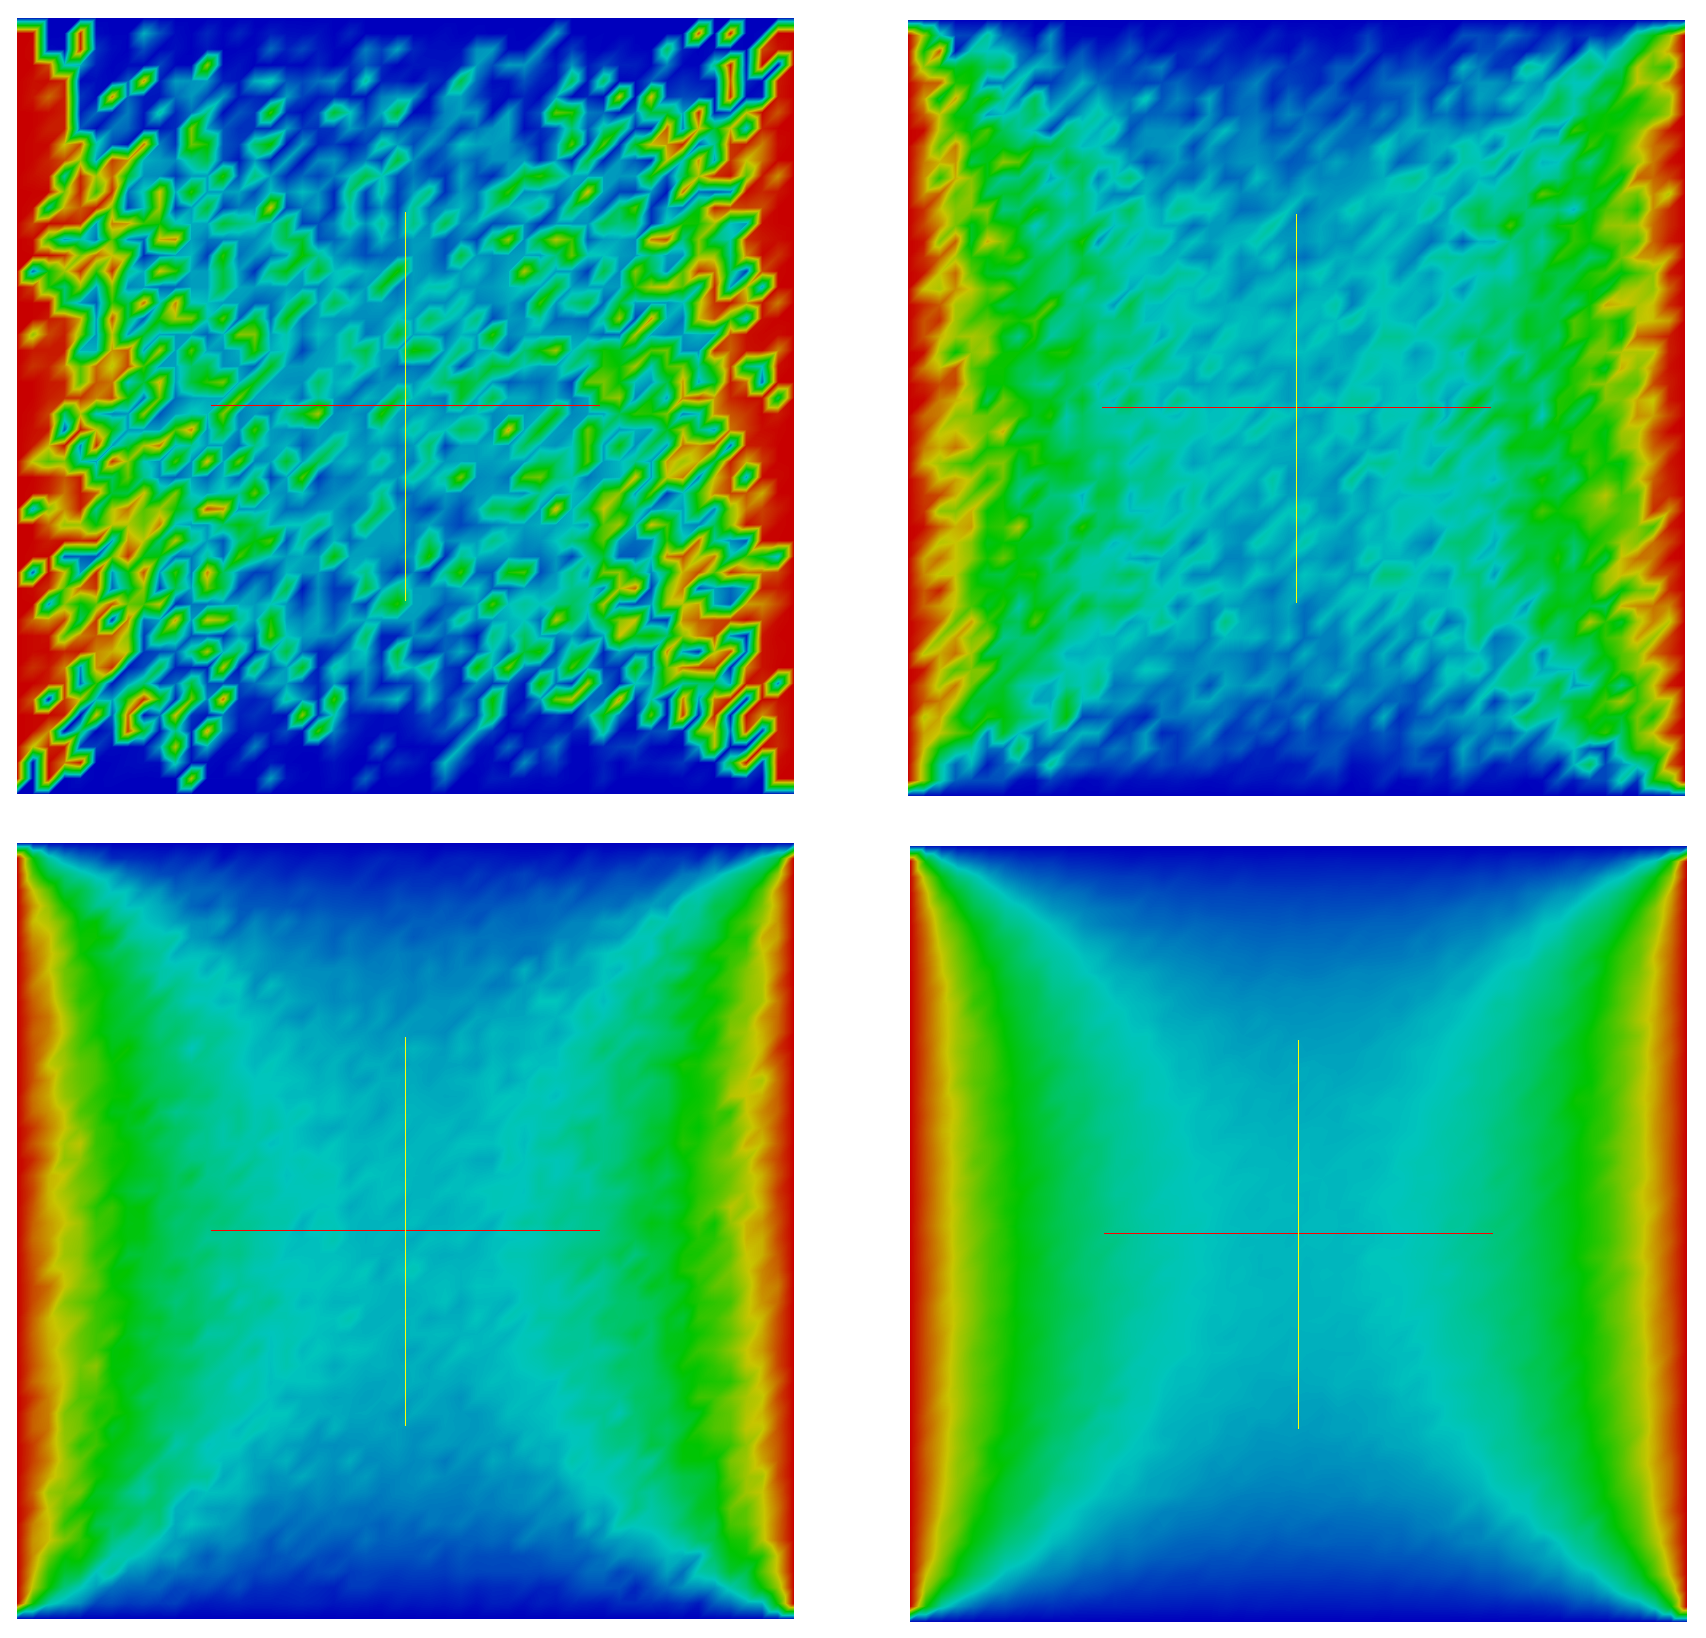
\includegraphics[width=6in]{chapters/mc_background/direct_evolution.png}
  \end{center}
  \caption{\textbf{Direct Monte Carlo solution to the heat equation
      with varying numbers of histories.} \textit{Top left: 1 history
      per state. Top right: 10 histories per state. Bottom left: 100
      histories per state. Bottom right: 1000 histories per state.}}
  \label{fig:direct_evolution}
\end{figure}
As the number of histories used per state is increased, the
statistical variance of the solutions is decreased as more tallies are
made. Starting with a single history at each state in the domain, the
high variance prevents a precise solution from being obtained although
we begin to see the solution take shape as expected. It is interesting
to note here that as the statistical uncertainty is reduced at each
grid point in the domain, the solution is resolved in a certain sense,
analogous to the convergence of a traditional iterative method.
\clearpage

\subsection{Adjoint Neumann-Ulam Method}
\label{sec:adjoint_mc}
An alternative to forward Monte Carlo matrix inversion is the adjoint
method. We begin by defining the linear system adjoint to
Eq~(\ref{eq:linear_problem}):
\begin{equation}
  \ve{A}^T \ve{y} = \ve{d}\:,
  \label{eq:adjoint_linear_problem}
\end{equation}
where $\ve{y}$ and $\ve{d}$ are the adjoint solution and source
vectors respectively and $\ve{A}^T$ is the adjoint operator for
$\ve{A} \in \mathbb{R}^{N \times N}$. We can split this equation to
mirror Eq~(\ref{eq:richardson_split}):
\begin{equation}
  \ve{y} = \ve{H}^T \ve{y} + \ve{d}\:.
  \label{eq:adjoint_split_system}
\end{equation}
As was required for convergence with the direct method using
Eq~(\ref{eq:richardson_split}), the spectral radius of $\ve{H}$ must
remain less than 1 as $\ve{H}^T$ contains the same eigenvalues and
therefore has the same spectral radius. By defining the following
adjoint inner product equivalence \cite{spanier_monte_1969}:
\begin{equation}
  \langle \ve{A}^T \ve{y}, \ve{x} \rangle = \langle \ve{y}, \ve{A}
  \ve{x} \rangle\:.
  \label{eq:adjoint_operator_product}
\end{equation}
it follows that:
\begin{equation}
  \langle \ve{x}, \ve{d} \rangle = \langle \ve{y}, \ve{b} \rangle\:.
  \label{eq:adjoint_vector_relation}
\end{equation}
Using these definitions, we can derive an estimator from the adjoint
method that will also give the solution vector, $\ve{x}$. As with the
direct method, we can acquire the adjoint solution by forming the
Neumann series by writing Eq~(\ref{eq:adjoint_split_system}) as:
\begin{equation}
  \ve{y} = (\ve{I} - \ve{H}^T)^{-1} \ve{d}\:,
  \label{eq:adjoint_split_system_2}
\end{equation}
which in turn yields the Neumann series using the adjoint operator:
\begin{equation}
  \ve{y} = \sum_{k=0}^{\infty} (\ve{H}^T)^k\ve{d}\:.
  \label{eq:adjoint_neumann_series}
\end{equation}
We expand this summation to again yield a series of transitions that
can be approximated by a Monte Carlo random walk sequence, this time
forming the Neumann series in reverse order:
\begin{equation}
  y_i = \sum_{k=0}^{\infty}\sum_{i_1}^{N}\sum_{i_2}^{N}\ldots
  \sum_{i_k}^{N}h_{i_k,i_{k-1}}\ldots h_{i_2,i_1} h_{i_1,i} d_{i_k}\:.
  \label{eq:adjoint_neumann_solution}
\end{equation}
We can readily build an estimator for the adjoint solution from this
series expansion, but we instead desire the solution to
Eq~(\ref{eq:linear_problem}). Here we have 2 unknowns, $\ve{y}$ and
$\ve{d}$, and therefore we require two constraints to close the
system. We use Eq~(\ref{eq:adjoint_vector_relation}) as the first
constraint and as a second constraint we select:
\begin{equation}
  \ve{d} = \boldsymbol{\delta}_j\:,
  \label{eq:adjoint_second_constraint}
\end{equation}
where $\boldsymbol{\delta}_j$ is one of a set of vectors in which the
$j^{th}$ component is the Kronecker delta function $\delta_{i,j}$. If
we apply Eq~(\ref{eq:adjoint_second_constraint}) to our first
constraint Eq~(\ref{eq:adjoint_vector_relation}), we get the following
convenient outcome:
\begin{equation}
  \langle \ve{y}, \ve{b} \rangle = \langle \ve{x},
  \boldsymbol{\delta}_j \rangle = x_j \:,
  \label{eq:inner_product_constraint}
\end{equation}
meaning that if we compute the inner product of the original source
and the adjoint solution using a delta function source, we recover one
component of the original solution.

In terms of radiation transport, this adjoint method is equivalent to
a traditional forward method where the initial state $i_0$ of the
random walk is determined by sampling the source vector $\ve{b}$ with
probabilities:
\begin{equation}
  P_{(i_0=i)}(\nu) = \frac{|b_i|}{||\ve{b}||_1}\:,
  \label{eq:adjoint_source_probability}
\end{equation}
with a random walk starting weight of:
\begin{equation}
  W_0 = ||\ve{b}||_1 \frac{b_i}{|b_i|}\:,
  \label{eq:adjoint_starting_weight}
\end{equation}
which gives the additional useful relation:
\begin{equation}
  b_{i_0} = W_0 P_{(i_0=i)}\:.
  \label{eq:adjoint_source_definition}
\end{equation}
As a result of using the adjoint system, we modify our probabilities
and weights using the \textit{adjoint Neumann-Ulam decomposition} of
$\ve{H}$:
\begin{equation}
  \ve{H}^{T} = \ve{P} \circ \ve{W}\:,
  \label{eq:adjoint_neumann_ulam}
\end{equation}
where now we are forming the decomposition with respect to the
transpose of $\ve{H}$. We then follow the same procedure as the direct
method for forming the probability and weight matrices in the
decomposition. Using the adjoint form, probabilities should instead be
column-scaled:
\begin{equation}
  p_{ij} = \frac{|h_{ji}|}{\sum_j |h_{ji}|}\:,
  \label{eq:adjoint_probability}
\end{equation}
such that we expect to select a new state, $j$, from the current state
in the random walk, $i$, by sampling column-wise (or row-wise if an
adjoint probability matrix is formed). Per
Eq~(\ref{eq:adjoint_neumann_ulam}), the transition weight is then
defined as:
\begin{equation}
  w_{ij} = \frac{h_{ji}}{p_{ij}}\:.
  \label{eq:adjoint_weight}
\end{equation}
Using the decomposition we can then define an expectation value for
the adjoint method. Given Eq~(\ref{eq:direct_permutation_weight}) as
the weight generated for a particular random walk permutation as in
Eq~(\ref{eq:mc_walk_permutation}) and our result from
Eq~(\ref{eq:inner_product_constraint}) generated by applying the
adjoint constraints, the contribution to the solution in state $j$
from a particular random walk permutation of $k$ events is then the
\textit{collision estimator}\footnote{The variance for this estimator
  is discussed in Appendix~\ref{chap:estimator_variance}.}:
\begin{equation}
  X_{j}(\nu) = \sum_{m=0}^k W_{m} \delta_{i_m,j}\:,
  \label{eq:adjoint_permutation_contribution}
\end{equation}
where the Kronecker delta indicates that the tally contributes only in
the current state, $i_m$, of the random walk.  Note here that the
estimator in Eq~(\ref{eq:adjoint_permutation_contribution}) does not
have a dependency on the source state as in
Eq~(\ref{eq:direct_permutation_contribution}), providing a remedy for
the situation in the direct method where we must start a random walk
in each source state for every permutation if we want to compute a
solution estimate for that state. In the adjoint method, we instead
tally in all states and those of lesser importance will not be visited
as frequently by the random walk. Finally, the expectation value using
all permutations is:
\begin{equation}
  E\{X_j\} = \sum_{\nu} P_{\nu} X_{j}(\nu)\:
  \label{eq:adjoint_expectation_value}
\end{equation}
which, if expanded in the same way as the direct method and utilizing
Eq~(\ref{eq:adjoint_source_definition}) to insert the source term,
directly recovers the exact solution:
\begin{equation}
  \begin{split}
    E\{X_j\} &=\sum_{k=0}^{\infty}\sum_{i_1}^{N}\sum_{i_2}^{N}\ldots
    \sum_{i_k}^{N} b_{i_0} p_{i_0,i_1}p_{i_1,i_2}\ldots
    p_{i_{k-1},i_k} w_{i_0,i_1}w_{i_1,i_2}\ldots
    w_{i_{k-1},i_k} \delta_{i_k,j} \\ &= x_{j}\:,
  \end{split}
  \label{eq:adjoint_expectation_expansion}
\end{equation}
therefore, also providing an unbiased Monte Carlo estimate of the
solution. It should be noted here that
Eq~(\ref{eq:adjoint_expectation_expansion}) only computes a single
component of our desired solution vector when really what we desire is
the entire solution vector. In an adjoint Monte Carlo simulation using
this estimator, the $w_{ij}$ elements that are added into the tally
for each state are only selected if/when the random walk currently
resides in that state. Much like a mesh tally in a particle transport
simulation, we have $N$ simultaneous tallies for $\ve{A} \in
\mathbb{R}^{N \times N}$ that will yield the entire solution vector.

Like the direct method, we also desire a criteria for random walk
termination for problems where only an approximate solution is
necessary. For the adjoint method, we utilize a \textit{relative
  weight cutoff}:
\begin{equation}
  W_f = W_c W_0\:,
  \label{eq:relative_weight_cutoff}
\end{equation}
where $W_c$ is defined as in the direct method. The adjoint random
walk will then be terminated after $m$ steps if $W_m < W_f$ as tally
contributions become increasingly small.

\subsubsection{Expected Value Estimator}
\label{subsec:expected_value_estimator}
In addition to the collision estimator, an additional estimator is
available due to the work of Okten \cite{okten_solving_2005} that uses
the method of expected values as a means to improve the Monte Carlo
estimate. As outlined by Spanier and Gelbard
\cite{spanier_monte_1969}, the method of expected values is a
deterministic averaging of events that may potentially occur in the
Monte Carlo random walk sequence. Okten applied this principle
directly to discrete Monte Carlo by forming the \textit{expected value
  estimator}\footnote{The variance for this estimator is discussed in
  Appendix~\ref{chap:estimator_variance}.} for a random walk of $k$
events:
\begin{equation}
  X_{j}(\nu) = b_j + \sum_{m=0}^k W_m h_{j,i_m}\,
  \label{eq:expected_value_estimator}
\end{equation}
where now the contribution of the iteration matrix is
deterministically averaged at step $m$ over all potential states $j$
that may be reached from the current state $i_m$. Via Okten, the
estimator can be shown to be unbiased through a comparison to the
collision estimator. We can first rewrite the summation in
Eq~(\ref{eq:expected_value_estimator}):
\begin{equation}
  X_{j}(\nu) = b_j + \sum_{m=0}^k \sum_{i=1}^N W_m
  \delta_{i_m,i} h_{ji}\,
  \label{eq:unbiased_eval_1}
\end{equation}
where $N$ is the number of states in the system. Immediately, we see
the collision estimator as defined by
Eq~(\ref{eq:adjoint_permutation_contribution}) and can therefore write
the expectation value as:
\begin{equation}
  E\{X_{j}\} = b_j + \sum_{i=1}^N E\{X_{i}\} h_{ji}\,
  \label{eq:unbiased_eval_2}
\end{equation}
which is equivalently is the $j^{th}$ component of
Eq~(\ref{eq:richardson_split}):
\begin{equation}
  E\{X_{j}\} = b_j + \sum_{i=1}^N x_{i} h_{ji}\,
  \label{eq:unbiased_eval_2}
\end{equation}
and is therefore an unbiased estimate. Compared to the collision
estimator, the expected value estimator provides additional
information at every step of the random walk, yielding potentially
better statistics with the same amount of transport
work. Conveniently, even if no Monte Carlo histories are computed, the
expected value estimator still deterministically computes the first
term of the Neumann Series, $\ve{H}^0\ve{b}$, whereas the collision
estimator will provide no information.

\subsubsection{Adjoint Method: Evolution of a Solution}
\label{subsec:adjoint_evolution}
As a means of visually demonstrating the adjoint Monte Carlo method,
again consider the 2-dimensional thermal diffusion problem with
sources on the left and right hand sides of the domain and a smaller
uniform source as shown in Figure~\ref{fig:heat_setup}. Using the
adjoint method with the collision estimator, the number of histories
sampled from the source was increased from 10 to 10,000,000 in order
to show its effects on the solution and the statistical nature of the
method. Figure~\ref{fig:adjoint_evolution} gives these results.
\begin{figure}[t!]
  \begin{center}
    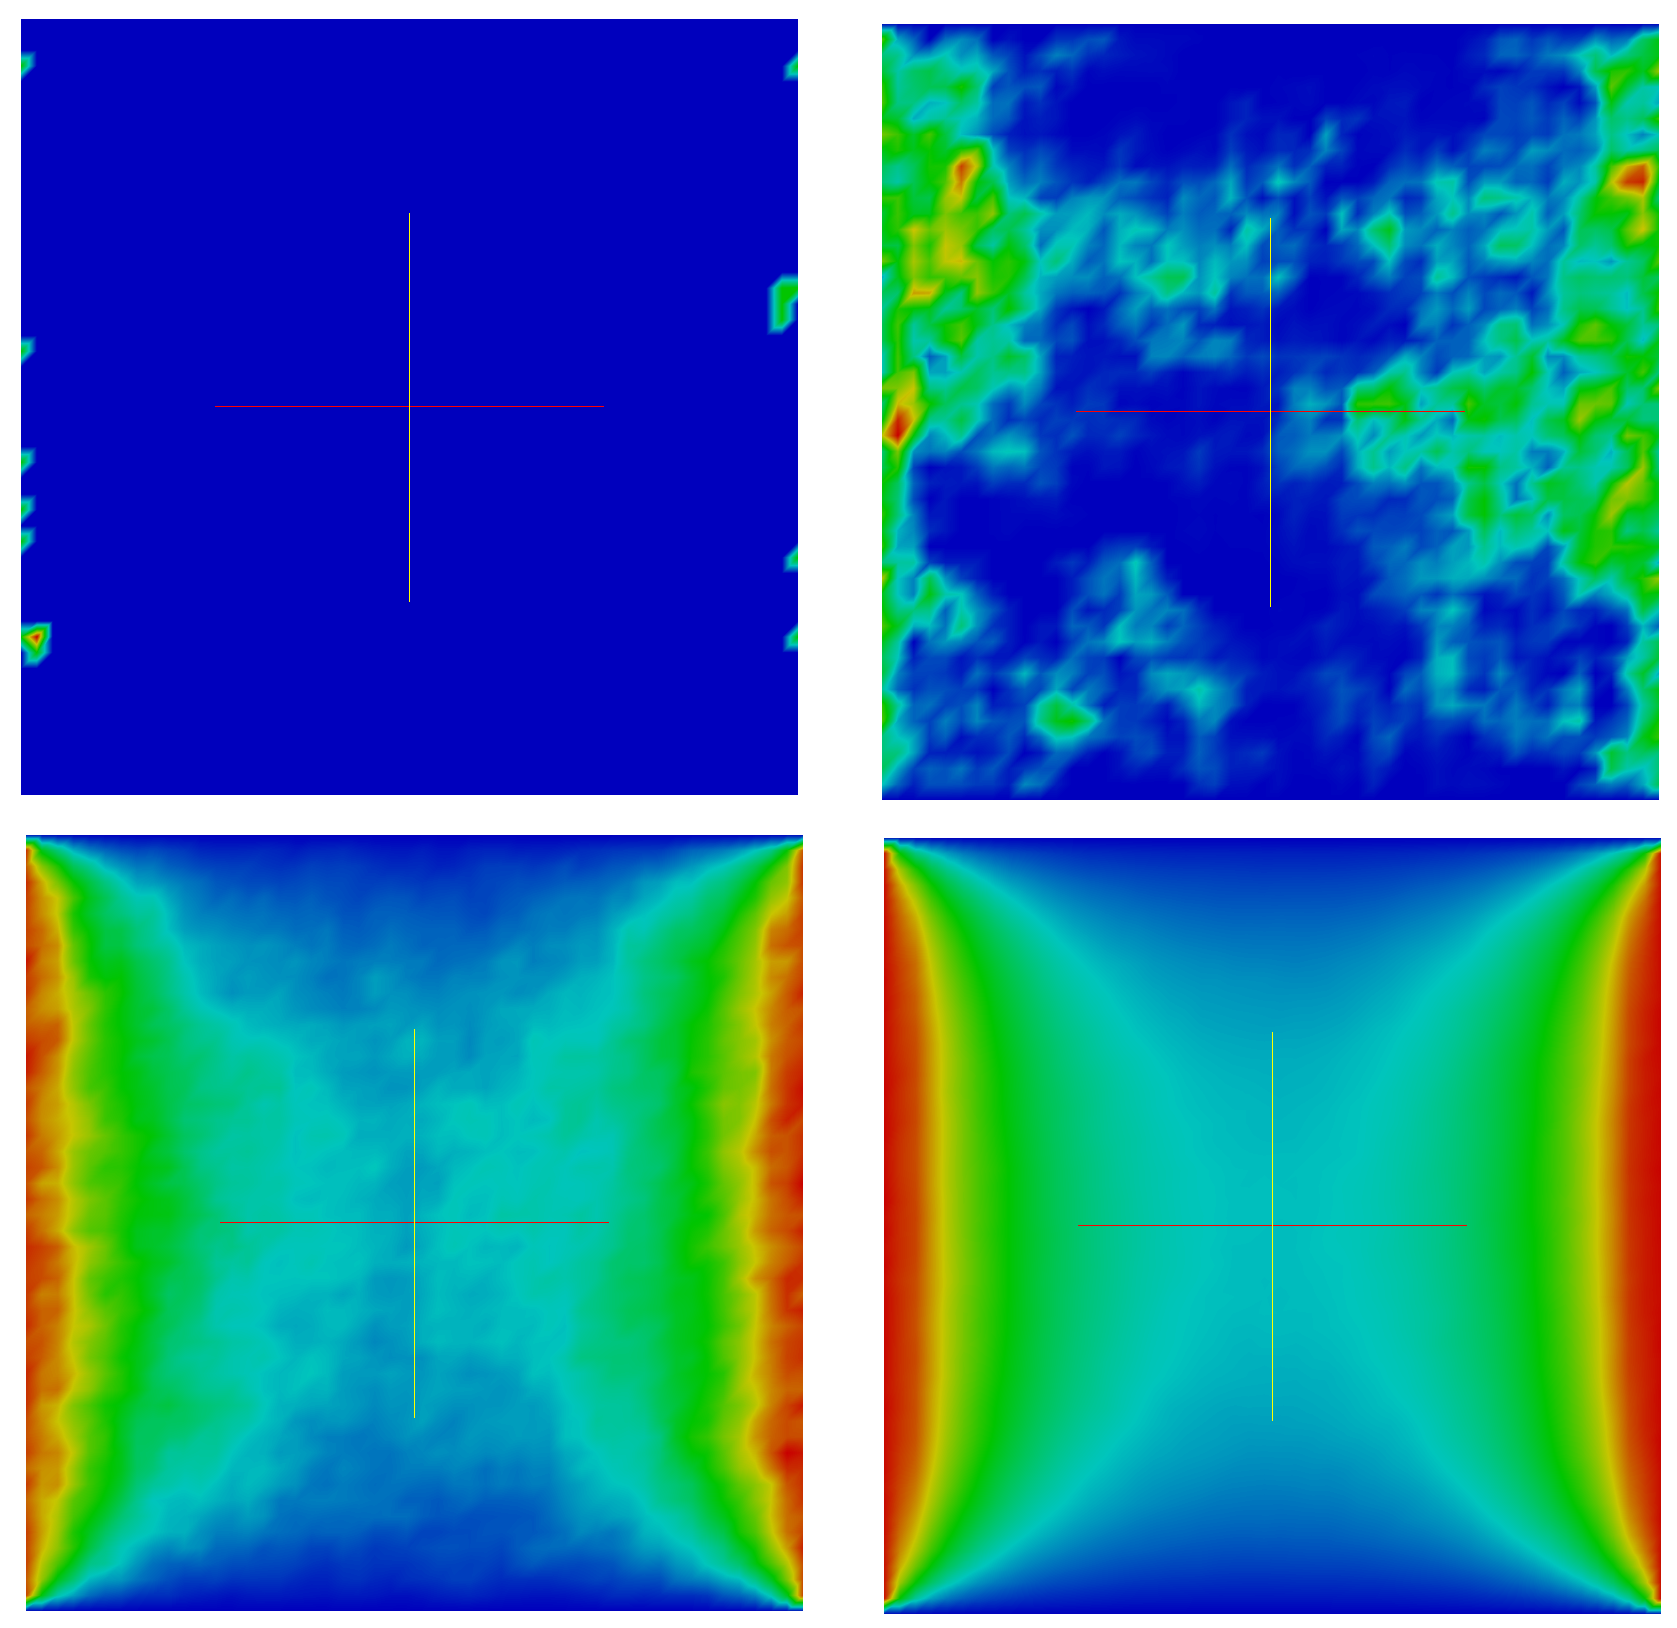
\includegraphics[width=6in]{chapters/mc_background/adjoint_evolution.png}
  \end{center}
  \caption{\textbf{Adjoint Monte Carlo solution to the heat equation
      with varying numbers of histories.} \textit{Top left: 10
      histories per state. Top right: 1,000 histories per
      state. Bottom left: 100,000 histories per state. Bottom right:
      10,000,000 histories per state.}}
  \label{fig:adjoint_evolution}
\end{figure}
As the number of histories used per state (or DOF) is increased, the
statistical variance of the solutions is decreased as more tally
contributions are made. At 10,000,000 histories per state, enough
information has been tallied to generate a reasonable estimate for the
structure of the solution. The visual difference between
Figures~\ref{fig:direct_evolution} and \ref{fig:adjoint_evolution} is
precisely that determined by their mathematics. As the adjoint
solution evolves with the addition of histories, more histories
emanate from the boundary the smaller uniform source in the domain
with more penetrating from the boundary into the domain and making
contributions to the tallies in those states as they are transported.

\clearpage

%%---------------------------------------------------------------------------%%
\section{Sequential Monte Carlo}
\label{sec:sequential_mc}
The direct and adjoint Neumann-Ulam methods described are limited by a
convergence rate of $1/\sqrt{N}$ by the Central Limit Theorem where
$N$ is the number of random walk permutations. In 1962, Halton
presented a residual Monte Carlo method that moves towards exponential
convergence rates \cite{halton_sequential_1962} and further refined
his work some years later \cite{halton_sequential_1994} with
applications of his work by the transport community confirming
exponential convergence rates \cite{evans_residual_2003}. Halton's
method, sequential Monte Carlo, utilizes the adjoint Monte Carlo
solver as a means of directly reducing the elements residual
vector. He proposed the following iterative scheme as a solution to
Eq~(\ref{eq:linear_problem})\:
\begin{subequations}
  \begin{gather}
    \ve{r}^k = \ve{b} - \ve{A}\ve{x}^k\:,\\  
    \ve{A}\boldsymbol{\delta}^{k} = \ve{r}^{k}\:,\\
    \ve{x}^{k+1} = \ve{x}^k + \boldsymbol{\delta}^{k}\:,
  \end{gather}
  \label{eq:sequential_monte_carlo}
\end{subequations}
where the correction $\boldsymbol{\delta}^k$ is computed by the
adjoint Monte Carlo method at each iteration. The merits of Halton's
approach are immediately visible in that we have now broken the
binding of the convergence rate to the Central Limit Theorem. Here,
the Monte Carlo solver is used to produce a correction from the
residual, analogous to using the residual to extract a correction from
the search subspace in a projection method. By doing this, the Monte
Carlo error is bound in the correction used to update the solution and
therefore does not explicitly manifest itself in the overall
convergence of the solution. The downside of such a method is that if
the solution guess is poor, then many iterations are required in order
to reach exponential converge as the Monte Carlo error (and therefore
the Central Limit Theorem) does dominate in this situation.

%%---------------------------------------------------------------------------%%
\section{Monte Carlo Synthetic Acceleration}
\label{sec:mcsa}
Using the ideas of Halton, Evans and Mosher recently developed a Monte
Carlo solution method that was not prohibited severely by the quality
of the initial guess for the system \cite{evans_monte_2009} and later
applied it more rigorously as a solution mechanism for the radiation
diffusion equation \cite{evans_monte_2012}. Their approach was instead
to use residual Monte Carlo as a synthetic acceleration for a
stationary method. To derive this method, we begin by splitting the
operator in Eq~(\ref{eq:linear_problem})
\begin{equation}
  \ve{x} = (\ve{I} - \ve{A})\ve{x} + \ve{b}\:.
  \label{eq:linear_split}
\end{equation}
With this we can then define the stationary method
\textit{Richardson's iteration} as:
\begin{equation}
  \ve{x}^{k+1} = (\ve{I} - \ve{A})\ve{x}^k + \ve{b}\:,
  \label{eq:richardsons_iteration}
\end{equation}
which will converge if $\rho(\ve{I} - \ve{A}) < 1$. We then define the
solution error at the $k^{th}$ iterate relative to the true solution:
\begin{equation}
  \delta \ve{x}^k = \ve{x} - \ve{x}^k\:.
  \label{eq:mcsa_error}
\end{equation}
Subtracting Eq~(\ref{eq:richardsons_iteration}) from
Eq~(\ref{eq:linear_split}) we get:
\begin{equation}
  \delta \ve{x}^{k+1} = (\ve{I} - \ve{A})\delta \ve{x}^k\:.
  \label{eq:mcsa_setup_1}
\end{equation}
Subtracting from this $(\ve{I} - \ve{A})\delta \ve{x}^{k+1}$ yields:
\begin{equation}
  \begin{split}
    \ve{A}\delta \ve{x}^{k+1} &= (\ve{I} -
    \ve{A})(\ve{x}^{k+1}-\ve{x}^{k}) \\ &= \ve{r}^{k+1}\:.
    \label{eq:mcsa_setup_2}
  \end{split}
\end{equation}
Using this, we define the following scheme that will converge in one
iteration if $\ve{A}$ is inverted exactly:
\begin{subequations}
  \begin{gather}
    \ve{x}^{k+1} = (\ve{I} - \ve{A})\ve{x}^k + \ve{b}\:,\\
    \ve{A} \delta \ve{x}^{k+1} = \ve{r}^{k+1}\:,\\
    \ve{x} = \ve{x}^{k+1} + \delta \ve{x}^{k+1}\:.
  \end{gather}
  \label{eq:mcsa_setup_3}
\end{subequations}
However, $\ve{A}$ is only approximately inverted by our numerical
methods and therefore we instead pose an iterative scheme in which the
Monte Carlo solvers are used to invert the operator. The
\textit{Fixed-Point Monte Carlo Synthetic Acceleration} (MCSA) method
is defined as:
\begin{subequations}
  \begin{gather}
    \ve{x}^{k+1/2} = \ve{x}^k + \ve{r}^k\:,\\
    \ve{r}^{k+1/2} = \ve{b} - \ve{A}\ve{x}^{k+1/2}\:,\\
    \ve{A}\delta\ve{x}^{k+1/2} = \ve{r}^{k+1/2}\:,\\
    \ve{x}^{k+1} = \ve{x}^{k+1/2} + \delta \ve{x}^{k+1/2}\:,\\
    \ve{r}^{k+1} = \ve{b} - \ve{A}\ve{x}^{k+1}\:,
  \end{gather}
  \label{eq:mcsa}
\end{subequations}
where a Neumann-Ulam Monte Carlo method is used to generate the
solution correction from the residual and Richardson's iteration in
the first step has been rewritten as a residual correction. Using
Monte Carlo in this way achieves the same effect as Halton's method,
decoupling its convergence rate from the overall convergence rate of
the method. Here, the approximate Monte Carlo solution is not driven
to a particular convergence as it merely supplies a correction for the
initial guess generated by Richardson's iteration. Rather, only a set
number of histories are required using the Neumann-Ulam method to
generate the correction. In addition, the fact that the scheme in
Eq~(\ref{eq:mcsa_setup_3}) will converge in one iteration if $\ve{A}$
is inverted exactly means that as more and more stochastic histories
are used to compute the correction and the error is reduced towards
zero, the number of iterations required for MCSA to converge should
decrease accordingly, thus accelerating the solution.

In addition to the Monte Carlo solver parameters dictating the number
of histories and weight cutoff, the outer MCSA iterations also have
the following stopping criteria:
\begin{equation}
  ||\ve{r}||_\infty < \epsilon \ ||\ve{b}||_\infty\:,
  \label{eq:mcsa_stopping_criteria}
\end{equation}
where $\epsilon$ is a user-defined parameter. As with any iterative
method, other stopping criteria using other vector norms could be
computed, however, for this work we will only use
Eq~(\ref{eq:mcsa_stopping_criteria}). We therefore have 3 parameters
to tune in an MCSA implementation: the number of Monte Carlo histories
computed in the Neumann-Ulam solve during each MCSA iteration, the
weight cutoff for those histories, and the total MCSA convergence
tolerance as specified by $\epsilon$.

\subsection{Alternative Fixed Point Iterations}
\label{subsubsec:alternative_fixed_point}
In addition to the basic Richardson iteration, the MCSA algorithm
presented in Eq~(\ref{eq:mcsa}) can be used to accelerate any fixed
point iteration which only depends on the state (typically the
residual) of the last iteration. As outlined in
Appendix~\ref{ch:linear_problem}, subspace methods take on a general
form using the Petrov-Galerkin conditions as constraints for
extracting a correction from the search subspace as given by
Eq~(\ref{eq:linear_projection_iteration}). Those that are
one-dimensional may be used with fixed-point MCSA as they only depend
the previous iteration for information. As an example, for
positive-definite but not necessarily symmetric problems, the minimal
residual iteration \cite{saad_iterative_2003} can be used in
conjunction with MCSA where the residual vector, $\mathbf{r}$, defines
the search subspace and the action of the linear operator on the
residual vector, $\mathbf{A}\mathbf{r}$, defines the constraint
subspace. Using this, we can then define an MCSA scheme that
accelerates the minimal residual iteration:
\begin{subequations}
  \begin{gather}
    \alpha = \frac{\langle \mathbf{A}\mathbf{r}^k, \mathbf{r}^k
      \rangle}{\langle \mathbf{A}\mathbf{r}^k, \mathbf{A}\mathbf{r}^k
      \rangle}\:, \\
    \ve{x}^{k+1/2} = \ve{x}^k + \alpha \ve{r}^k\:,
    \label{eq:min_res_correction}\\
    \ve{r}^{k+1/2} = \ve{b} - \ve{A}\ve{x}^{k+1/2}\:,\\ 
    \ve{A}\delta\ve{x}^{k+1/2} = \ve{r}^{k+1/2}\:,\\ 
    \ve{x}^{k+1} = \ve{x}^{k+1/2} + \delta\ve{x}^{k+1/2}\:,\\ 
    \ve{r}^{k+1} = \ve{b} - \ve{A}\ve{x}^{k+1}\:.
  \end{gather}
  \label{eq:mcsa_min_res}
\end{subequations}
where $\alpha$ is an optimal extrapolation parameter generated from
the constraints. Interestingly, this scheme is nearly identical to the
Richardson iteration version in Eq~(\ref{eq:mcsa}) except now the
additional extrapolation parameter, $\alpha$, is applied to the
residual correction in Eq~(\ref{eq:min_res_correction}) as a means of
selecting a more optimal search direction at each iteration,
potentially further improving convergence.

\subsection{Preconditioning MCSA}
\label{subsec:stochastic_preconditioning}
In most cases, at least a minimal amount of \textit{preconditioning}
of the linear system will be required in order to use the class of
stochastic methods described. Although these methods have no symmetry
requirements for convergence, they do require that the spectral radius
of the iteration matrix be less than one. Preconditioning serves as a
means of achieving this by altering the eigenvalue spectrum of the
iteration matrix.

\subsubsection{Basic Preconditioning}
\label{subsubsec:basic_mcsa_preconditioning}
As an example of basic preconditioning, to achieve a spectral radius
of less than one for diagonally dominant matrices point Jacobi
preconditioning can be used such that the preconditioning matrix
$\ve{M}$ is:
\begin{equation}
  \ve{M} = diag(\ve{A})\:,
  \label{eq:jacobi_preconditioner}
\end{equation}
which may be trivially inverted. With the application of this
preconditioner we are instead solving the following scaled linear
system:
\begin{equation}
  \ve{M}^{-1}\ve{A}\ve{x} = \ve{M}^{-1}\ve{b}\:.
  \label{eq:jacobi_precond_linear_problem}
\end{equation}
Next, we can apply MCSA to solve
Eq~(\ref{eq:jacobi_precond_linear_problem}): 
\begin{subequations}
  \begin{gather}
    \ve{x}^{k+1/2} = \ve{x}^k +
    \ve{M}^{-1}\ve{r}^k\:,\\ \ve{r}^{k+1/2} =
    \ve{b}-\ve{A}\ve{x}^{k+1/2}\:,\\ \ve{M}^{-1}\ve{A}\delta\ve{x}^{k+1/2}
    = \ve{M}^{-1}\ve{r}^{k+1/2}\:,\\ \ve{x}^{k+1} = \ve{x}^{k+1/2} +
    \delta \ve{x}^{k+1/2}\:,\\
    \ve{r}^{k+1} = \ve{b} - \ve{A}\ve{x}^{k+1}\:,
    \label{eq:jacobi_preconditioned_mcsa}
  \end{gather}
\end{subequations}
where the Neumann-Ulam Monte Carlo solve now has a preconditioned
operator from which to build weights and probabilities for transport
and a preconditioned source vector to sample.

Choosing point Jacobi preconditioning with MCSA is advantageous for
several reasons. First, $\rho(\ve{I} - \ve{M}^{-1}\ve{A}) < 1$ is true
for all $\ve{A}$ that is diagonally dominant and is easy to formulate
because the inversion of $\ve{M}$ is trivial. Second, because the
Monte Carlo method used within MCSA to compute the correction operates
on a linear problem with the preconditioned operator, then $\ve{H}$ in
the Neumann-Ulam solver will have a zero term in each of its diagonal
elements, thereby eliminating all in-state transitions during the
random walk sequence. Because of this, point Jacobi preconditioning
should be considered for many classes of problems, regardless of any
other preconditioning that is applied to the system. In addition,
Jacobi preconditioning has been shown to be an effective
preconditioning mechanism for MCSA when used with the thermal
radiation diffusion equation \cite{evans_monte_2012}.

\clearpage

\subsubsection{General Preconditioning Strategies}
\label{subsubsec:general_mcsa_preconditioning}
It is possible to use general left, right, and left/right
preconditioning with MCSA by carefully considering the underlying
Monte Carlo problem that will be solved with the Neumann-Ulam
method. We consider here the general left/right preconditioned method
as the left or right preconditioned methods can be inferred from its
formulation. We consider a left preconditioner $\ve{M_L}$ and a right
preconditioner $\ve{M_R}$. The left/right preconditioned linear
problem is then:
\begin{equation}
  \ve{M}_L^{-1}\ve{A}\ve{M}_R^{-1}\ve{M}_R\ve{x} = \ve{M}_L^{-1}\ve{b}\:.
  \label{eq:left_right_linear_problem}
\end{equation}
To handle the right preconditioning, the system is written with a
substitution of variables:
\begin{equation}
  \ve{M}_L^{-1}\ve{A}\ve{M}_R^{-1}\ve{u} = \ve{M}_L^{-1}\ve{b}\:,
  \label{eq:left_right_subs_problem}
\end{equation}
with
\begin{equation}
  \ve{x} = \ve{M}_R^{-1}\ve{u}\:.
  \label{eq:left_right_recover}
\end{equation}
To apply such a method to MCSA, we solve for the substituted variable
$\ve{u}$ during the iteration sequence:
\begin{subequations}
  \begin{gather}
    \ve{u}^{k+1/2} = \ve{u}^k + \ve{r}^k\:,\\
    \ve{r}^{k+1/2} = \ve{M}_L^{-1}(\ve{b}-\ve{A}\ve{M}_R^{-1}\ve{u}^{k+1/2})\:,\\ 
    \ve{M}_L^{-1}\ve{A}\ve{M}_R^{-1}\delta\ve{u}^{k+1/2} = \ve{r}^{k+1/2}\:,\\ 
    \ve{u}^{k+1} = \ve{u}^{k+1/2} + \delta \ve{u}^{k+1/2}\:,\\
    \ve{r}^{k+1} = \ve{M}_L^{-1}(\ve{b}-\ve{A}\ve{M}_R^{-1}\ve{u}^{k+1})\:,
  \end{gather}
  \label{eq:left_right_mcsa}
\end{subequations}
and then recover the original solution vector with
Eq~(\ref{eq:left_right_recover}) after convergence. For the Monte
Carlo problem, we isolate the generation of the correction:
\begin{equation}
  \ve{M}_L^{-1}\ve{A}\ve{M}_R^{-1}\delta\ve{u}^{k+1/2} = \ve{r}^{k+1/2}\:,
  \label{eq:left_right_correction}
\end{equation}
and note that the preconditioned residual of the substituted variable
is now serving as the source and the new iteration matrix is:
\begin{equation}
  \ve{H} = \ve{I} - \ve{M}_L^{-1}\ve{A}\ve{M}_R^{-1}\:.
  \label{eq:left_right_iteration_matrix}
\end{equation}
As we require $(i,j)$ element-wise access to the iteration matrix in
order to construct probabilities and weights for the Monte Carlo
procedure from the Neumann-Ulam decomposition, the \textit{composite
  operator}, $\ve{M}_L^{-1}\ve{A}\ve{M}_R^{-1}$, must be formed via
matrix-matrix multiplication. 

Several possible shortcomings of this preconditioning approach are
readily observed. First, the matrix-matrix multiplication operation
for sparse, parallel distributed matrices is significantly more
expensive than a matrix-vector multiplication operation. Second, each
preconditioner must be explicitly inverted, an operation in itself
that may be expensive and which prohibits the use of any
preconditioners which provide no mechanism to extract their
inverse. Third, for many modern preconditioning methods, this
inversion may yield dense matrices, destroying sparsity and further
impeding the performance of a matrix-matrix multiplication
operation. It is also interesting to note that the Monte Carlo problem
in the general left/right preconditioned scheme given by
Eq~(\ref{eq:left_right_correction}) is not fully left/right
preconditioned (meaning that we do not recover $\ve{x}$), but instead
part of a sequence for finding the substituted variable $\ve{u}$. We
do, however, gain the benefits of this general preconditioning by
building the iteration matrix in
Eq~(\ref{eq:left_right_iteration_matrix}) from the fully
preconditioned linear operator. In addition, for MCSA to apply to
increasingly difficult problems, more advanced preconditioning
techniques that require the generation of the composite operator may
be necessary for convergence.

%%---------------------------------------------------------------------------%%
\section{Monte Carlo Synthetic Acceleration Analysis}
\label{sec:mcsa_analysis}
In this section we analyze the effects of various MCSA parameters to
better our understanding of the algorithm and facilitate future
work. In addition, we demonstrate the effectiveness of MCSA as
compared to Halton's Sequential Monte Carlo method. To do this, we
choose the two-dimensional time-dependent Poisson equation as a simple
model transport problem\footnote{The Poisson equation is a simple form
  of the diffusion equation and has a similar elliptic character in
  its time-dependent form to the neutron transport equations that will
  be solved in the next chapter.}:
\begin{equation}
  \frac{\partial \ve{u}}{\partial t} = \nabla^2 \ve{u}\:.
  \label{eq:poisson_equation}
\end{equation}
For all comparisons, a single time step is computed with backwards Euler time
integration. The Laplacian is differenced on a square Cartesian grid with a
second-order five-point stencil,
\begin{equation}
  \nabla^2_5 = \frac{1}{\Delta^2}[u_{i-1,j} + u_{i+1,j} + u_{i,j-1} +
    u_{i,j+1} - 4 u_{i,j}]\:,
  \label{eq:five_point_stencil}
\end{equation}
and a fourth-order nine-point stencil,
\begin{multline}
  \nabla^2_9 = \frac{1}{6\Delta^2}[4 u_{i-1,j} + 4 u_{i+1,j} + 4
    u_{i,j-1} + 4 u_{i,j+1} + u_{i-1,j-1}\\ + u_{i-1,j+1} +
    u_{i+1,j-1} + u_{i+1,j+1} - 20 u_{i,j}]\:,
  \label{eq:nine_point_stencil}
\end{multline}
both assuming a grid size of $\Delta$ in both the $i$ and $j$ directions. For
a single time step solution, we then have the following sparse linear system
to be solved with the MCSA method:
\begin{equation}
  \ve{A} \ve{u}^{n+1} = \ve{u}^n\:.
  \label{eq:poisson_eq_lin_sys}
\end{equation}
Both the stencils will be used to vary the size and density of the sparse
linear system in Eq.~(\ref{eq:poisson_eq_lin_sys}).

\subsection{Monte Carlo Method Selection}
\label{sec:mc_method_selection}
The MCSA method defined in Eq.~(\ref{eq:mcsa}) uses the adjoint method
to estimate the error in a residual Monte Carlo solve instead of the
direct method outlined in \S\ref{sec:direct_mc}. To demonstrate the
effectiveness of the adjoint method over the direct method within the
context of MCSA, we solve Poisson equation in a series of numerical
experiments. A timing and convergence study is used to demonstrate
the effectiveness of the adjoint method with the collision estimator
as compared to the direct method. To assess both the CPU time and
number of iterations required to converge to a solution, a problem of
constant $\Delta$ was used with varying values of the number of mesh
elements, fixing the spectral radius of the system at a constant value
for each variation. Both the five-point and nine-point stencils were
used with both the direct and adjoint solvers. For each case, $N
\times N$ total random walk permutations were computed per MCSA
iteration where $N \times N$ is the number of discrete grid points (or
degrees of freedom) in the system. Solver parameters were set to a
weight cutoff of \sn{1}{-4} for the stochastic linear solver and a
convergence tolerance of \sn{1}{-8} for the MCSA iterative solver.
Figure~\ref{fig:poisson_cpu_time} gives the CPU time needed for each
case to converge in seconds, and Figure~\ref{fig:poisson_iterations}
gives the number of iterations needed for each case to converge to the
specified tolerance, both as a function of the problem size. All
computations presented in this section and the remaining sections of
this chapter were completed on a 3.0 GHz Intel Core 2 Quad Q9650 CPU
machine with 16 GB 1067 MHz DDR3 memory.

\begin{figure}[t!]
  \centering
  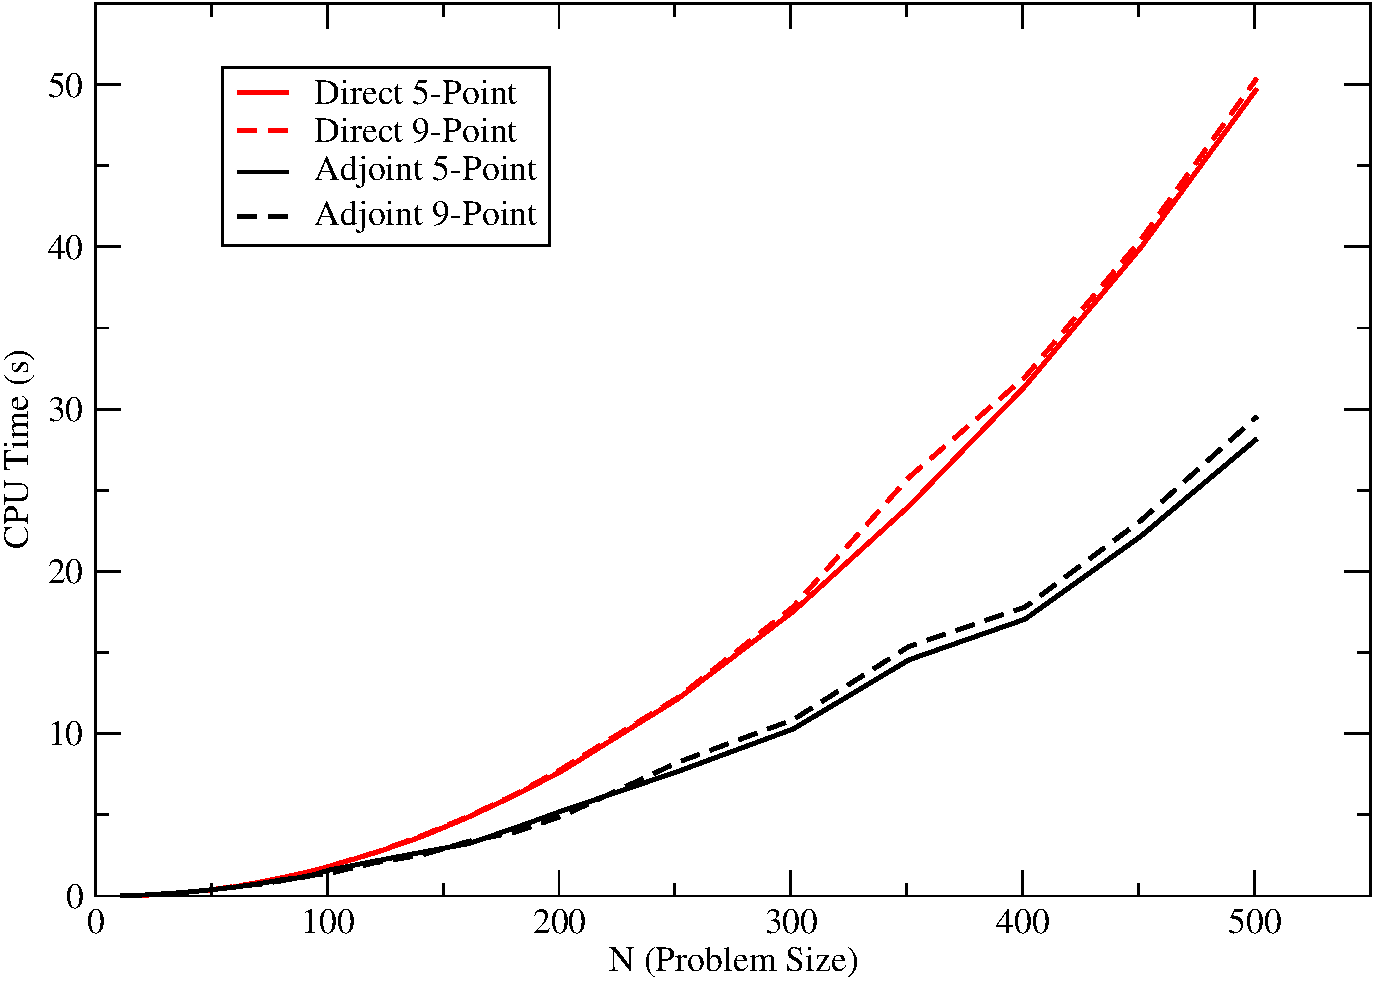
\includegraphics[width=5in,clip]{chapters/mc_background/dir_adj_cpu.pdf}
  \caption{\textbf{CPU Time (s) to converge vs. Problem Size ($N$ for
      an $N \times N$ square mesh).} \textit{Both the adjoint and
      direct solvers are used with the five point and nine point
      stencils. A CPU time speedup is noted with the adjoint method
      due to the higher density of random walk events in regions with
      a large residual.}}
  \label{fig:poisson_cpu_time}
\end{figure}

\begin{figure}[t!]
  \centering
  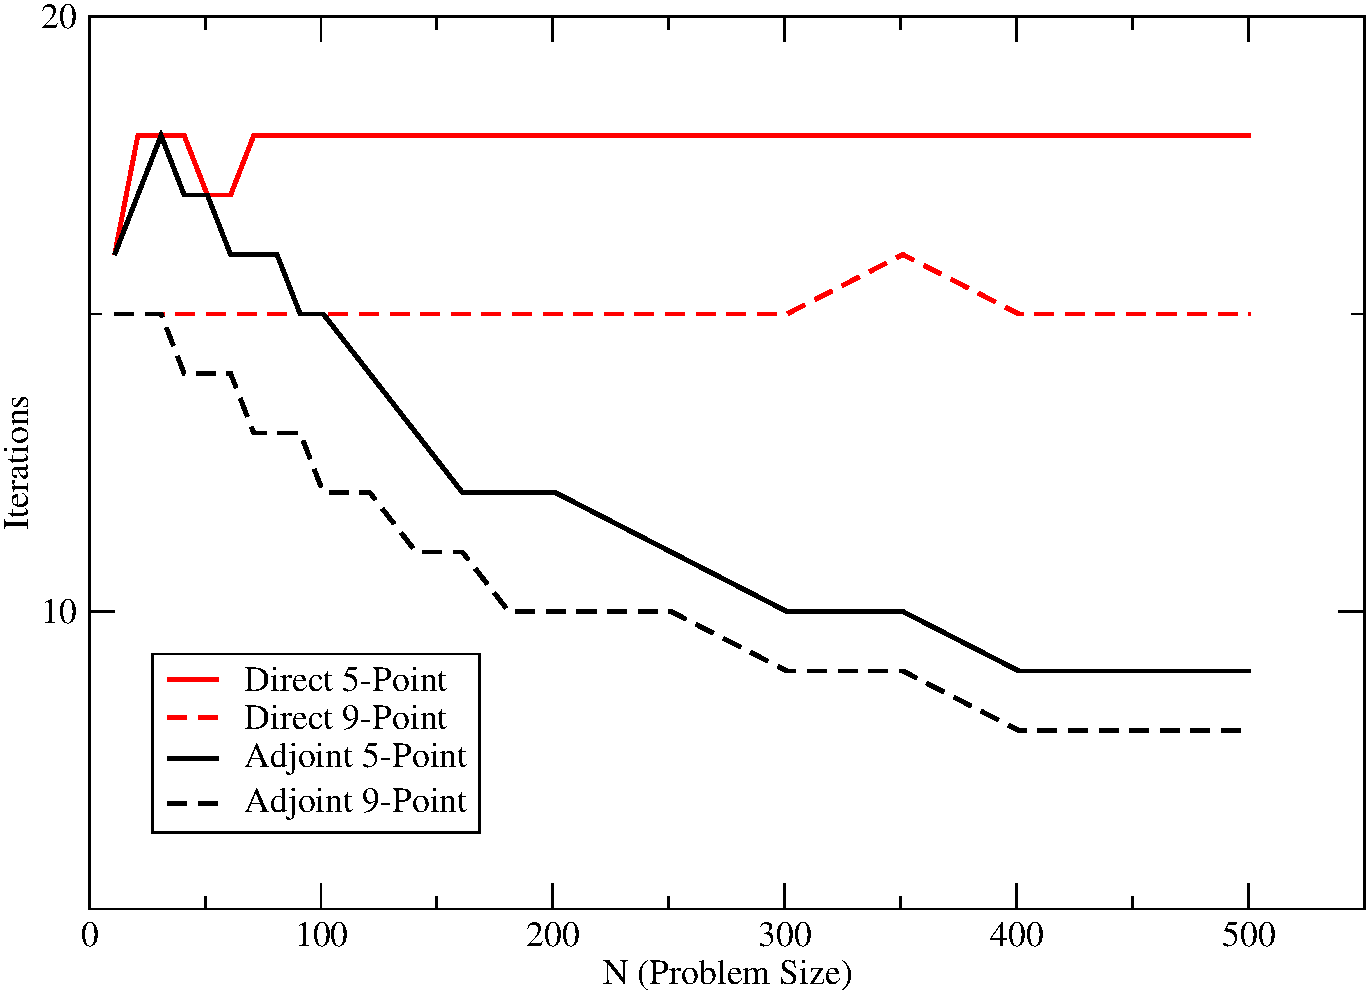
\includegraphics[width=5in,clip]{chapters/mc_background/dir_adj_iterations.pdf}
  \caption{\textbf{Iterations to converge vs. Problem Size ($N$ for an
      $N \times N$ square mesh).} \textit{Both the adjoint and direct
      solvers are used with the five-point and nine-point stencils.}}
  \label{fig:poisson_iterations}
\end{figure}

We see clearly in Figure~\ref{fig:poisson_cpu_time} that the using the
adjoint solver with MCSA results in a speedup over the direct solver
while the number of iterations required to converge is also reduced as
shown in Figure~\ref{fig:poisson_iterations}. We expect this for
several reasons. First, with an equivalent number of histories
specified for both solvers per MCSA iteration and a system of size $N
\times N$, the direct solver will compute a single random walk for
each state in the system per iteration to acquire a solution in that
state. This is necessary in the direct method to ensure a contribution
from each state as the random walk sequence will only contribute to
the starting state. For the adjoint method, a total of $N \times N$
random walk events will have their starting state determined by
sampling the residual vector. Because the random walk sequence
contributes to the state in which it currently resides, sampling the
residual vector as the Monte Carlo source gives a higher density of
random walk events in regions with a high residual, thus giving a more
accurate correction in that region due to reduced statistical
error. 

From an iteration perspective, Figure~\ref{fig:poisson_iterations}
shows that using the direct method yields a roughly unchanging number
of iterations required to converge as the problem size
increases. Again, if we desire a correction value for all states in
the problem, then we must start a random walk in each state in the
system without taking into account the structure of the residual
vector. Because of this, as the problem size grows adding histories is
ineffective as many are added in states where the error is smaller
than in other parts of the problem, ultimately not reducing the number
of iterations needed to converge. Conversely, as the problem size
grows in the adjoint method, the additional stochastic histories that
will be computed are concentrated in regions with a large residual,
further reducing the stochastic error in the correction in those
regions and subsequently reducing the required number of iterations to
converge.

As an additional comparison, the convergence behavior of MCSA can be
analyzed using both the adjoint and direct solvers to detect any
performance benefits. To assess the convergence properties of MCSA
using each solver and stencil, the infinity norm of the residual
computed in Eq.~(\ref{eq:mcsa}) was collected at each iteration for a
fixed problem size of $N=500$. Figure~\ref{fig:poisson_convergence}
gives the results of these computations. We note that using the
adjoint method with the same number of stochastic histories per MCSA
iteration gives a faster rate of converge for the same reasons as
above. We also note here that fewer iterations are required for
convergence when the 9-point stencil is used to discretize the
Laplacian operator (although at no gain in speed as given by the
results in Figure~\ref{fig:poisson_cpu_time}). This is due to the fact
that the smaller discretization error directly corresponds to a more
well defined residual source generated by the Richardson extrapolation
for the Monte Carlo calculation. In addition, the better defined
source is transported through a domain described more accurately by
the 9-point stencil, thus yielding a more accurate correction vector
from the Monte Carlo calculation.

\begin{figure}[t!]
  \centering
  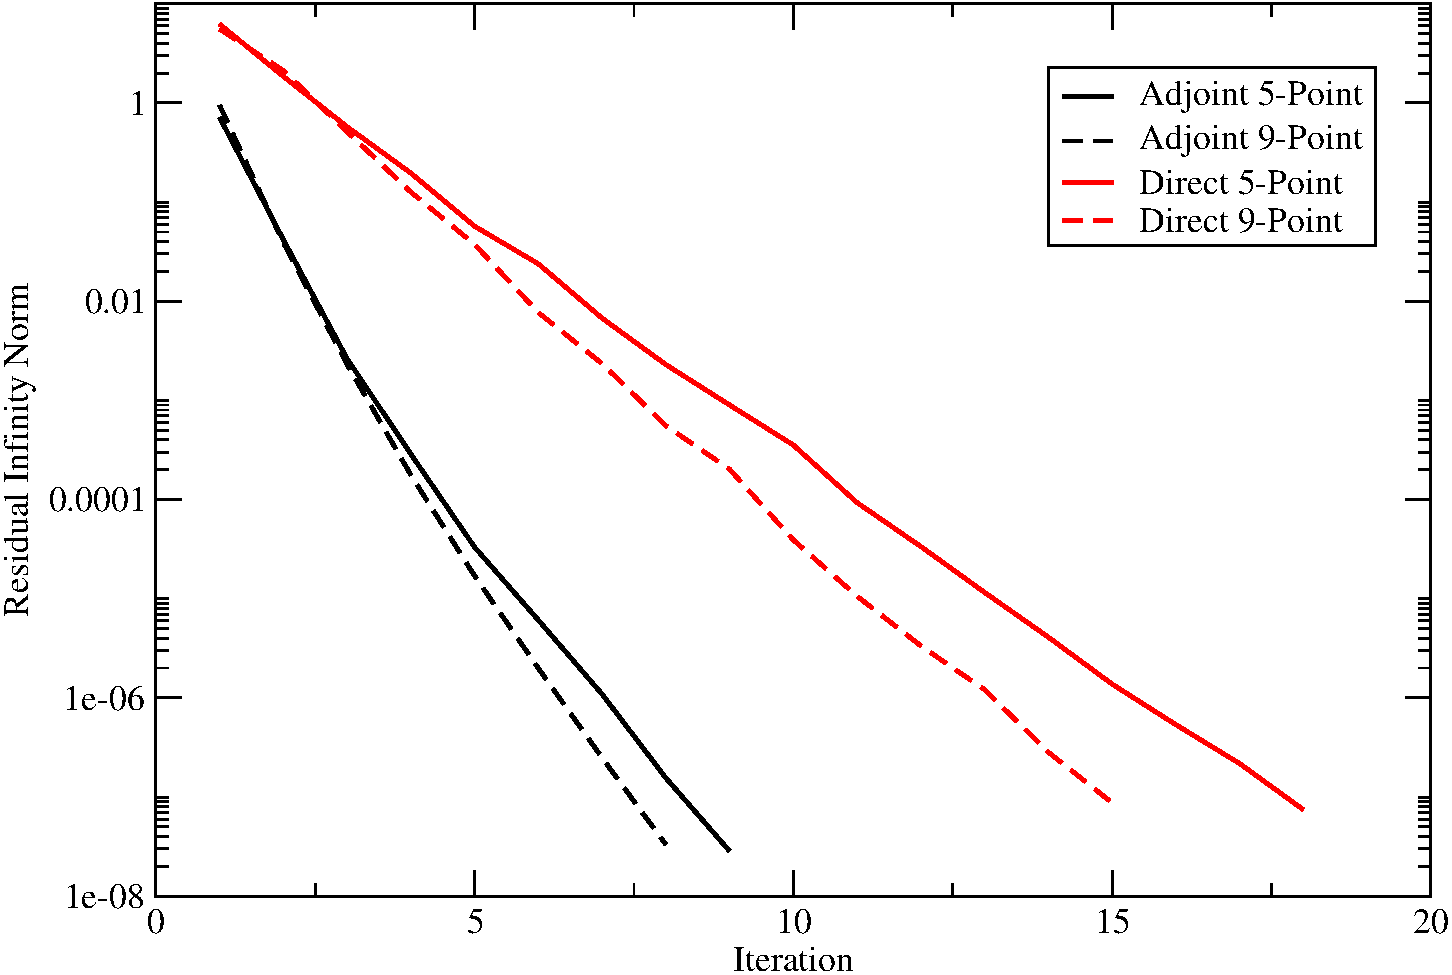
\includegraphics[width=5in,clip]{chapters/mc_background/dir_adj_conv.pdf}
  \caption{\textbf{Infinity norm of the solution residual
      vs. iteration number for a problem of size $N=500$.}
    \textit{Both the adjoint and direct solvers are used with the five
      point and nine point stencils. A higher rate of convergence is
      observed for MCSA using the adjoint Monte Carlo solver as
      compared to the direct method when both solvers compute the same
      number of random walks per iteration.}}
  \label{fig:poisson_convergence}
\end{figure}

\subsection{MCSA Comparison to Sequential Monte Carlo}
\label{subsec:sequential_comparison}
To further motivate using Monte Carlo Synthetic Acceleration, we
compare its performance to Halton's Sequential Monte Carlo. For this
comparison, we use the same transient Poisson problem as described in
the previous section and choose only the 5-point stencil to discretize
the Laplacian operator as the previous results yielded little
qualitative difference between the discretizations. Both MCSA and
Halton's method are used with the adjoint Monte Carlo solver and the
collision estimator. In order to complete the same study as in the
previous section, the number of histories computed by the Monte Carlo
solver at each iteration had to be doubled to $2 \times N \times N$ in
order to ensure convergence in Sequential Monte Carlo Method. For the
majority of the problems in the previous section, the Sequential
method used with $N \times N$ histories would not converge.

Figure~\ref{fig:seq_cpu_time} gives the CPU time results for this
comparison as a function of problem size while
Figure~\ref{fig:seq_iterations} gives the number of iterations to
converge as a function of problem size with a convergence tolerance of
\sn{1}{-8}. In both cases, using the Monte Carlo solver as a synthetic
acceleration rather than in a pure residual Monte Carlo scheme
resulted in a reduction in both CPU time and iterations required to
converge. The additional Richardson extrapolation between each Monte
Carlo solve in the MCSA method gives a better converged residual
source to use with the Monte Carlo calculation while the Sequential
method requires more iterations to achieve the same level of
convergence in the residual.

\begin{figure}[t!]
  \centering
  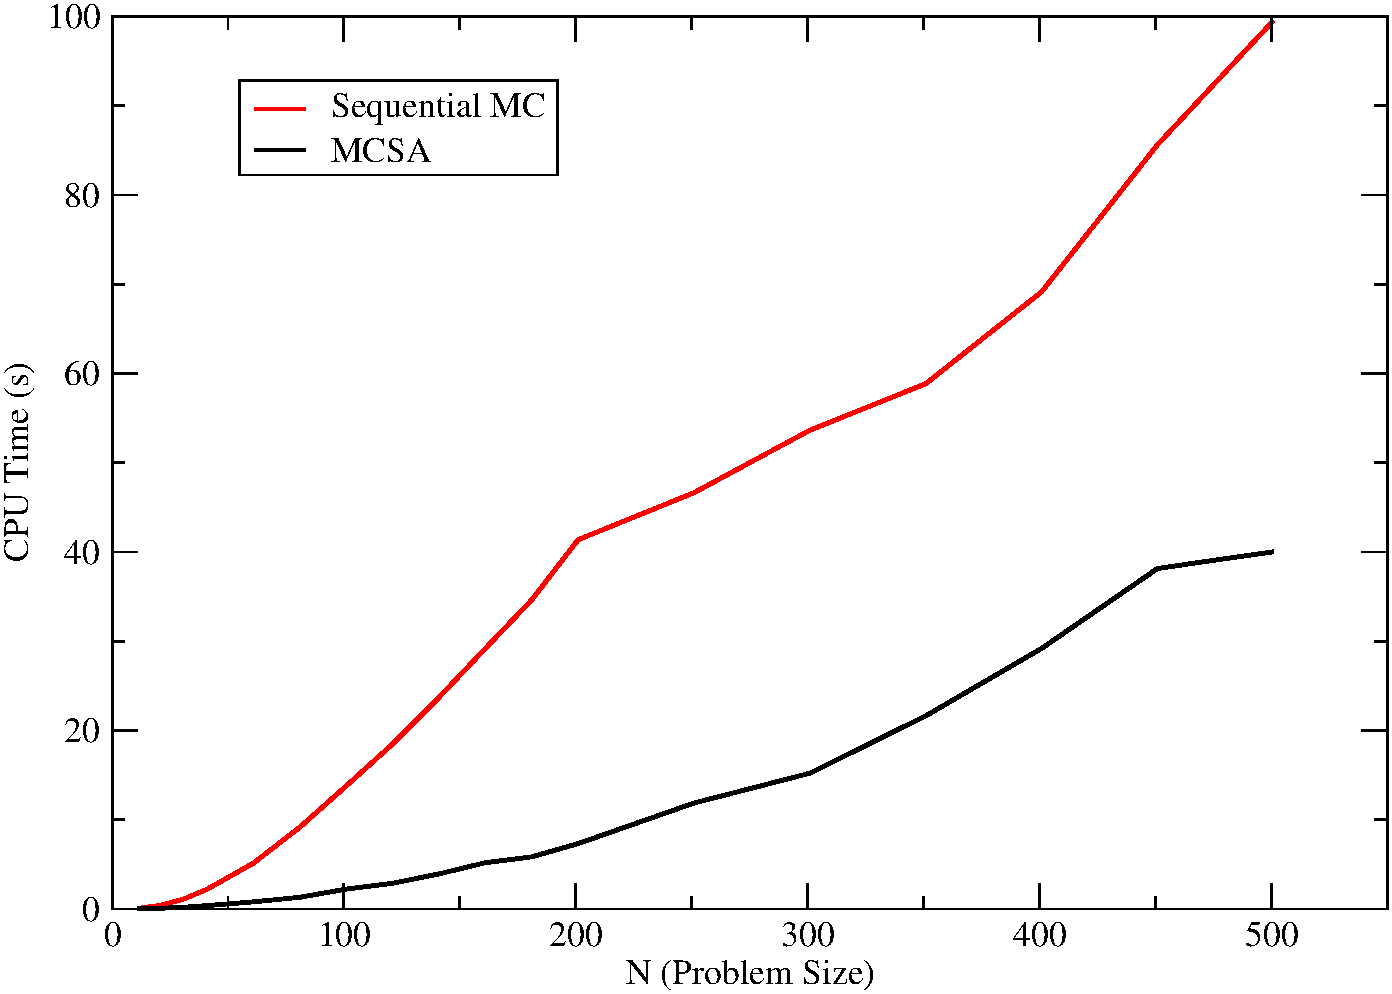
\includegraphics[width=4.5in,clip]{chapters/mc_background/seq_cpu.pdf}
  \caption{\textbf{CPU Time (s) to converge vs. Problem Size ($N$ for
      an $N \times N$ square mesh).} \textit{Both the Sequential Monte
      Carlo and MCSA solvers are used with the five point stencils and
      the adjoint Monte Carlo solver. The number of random walks was
      twice the number of discrete states in the system in order to
      ensure convergence in the Sequential Monte Carlo method.}}
  \label{fig:seq_cpu_time}
\end{figure}

\begin{figure}[t!]
  \centering
  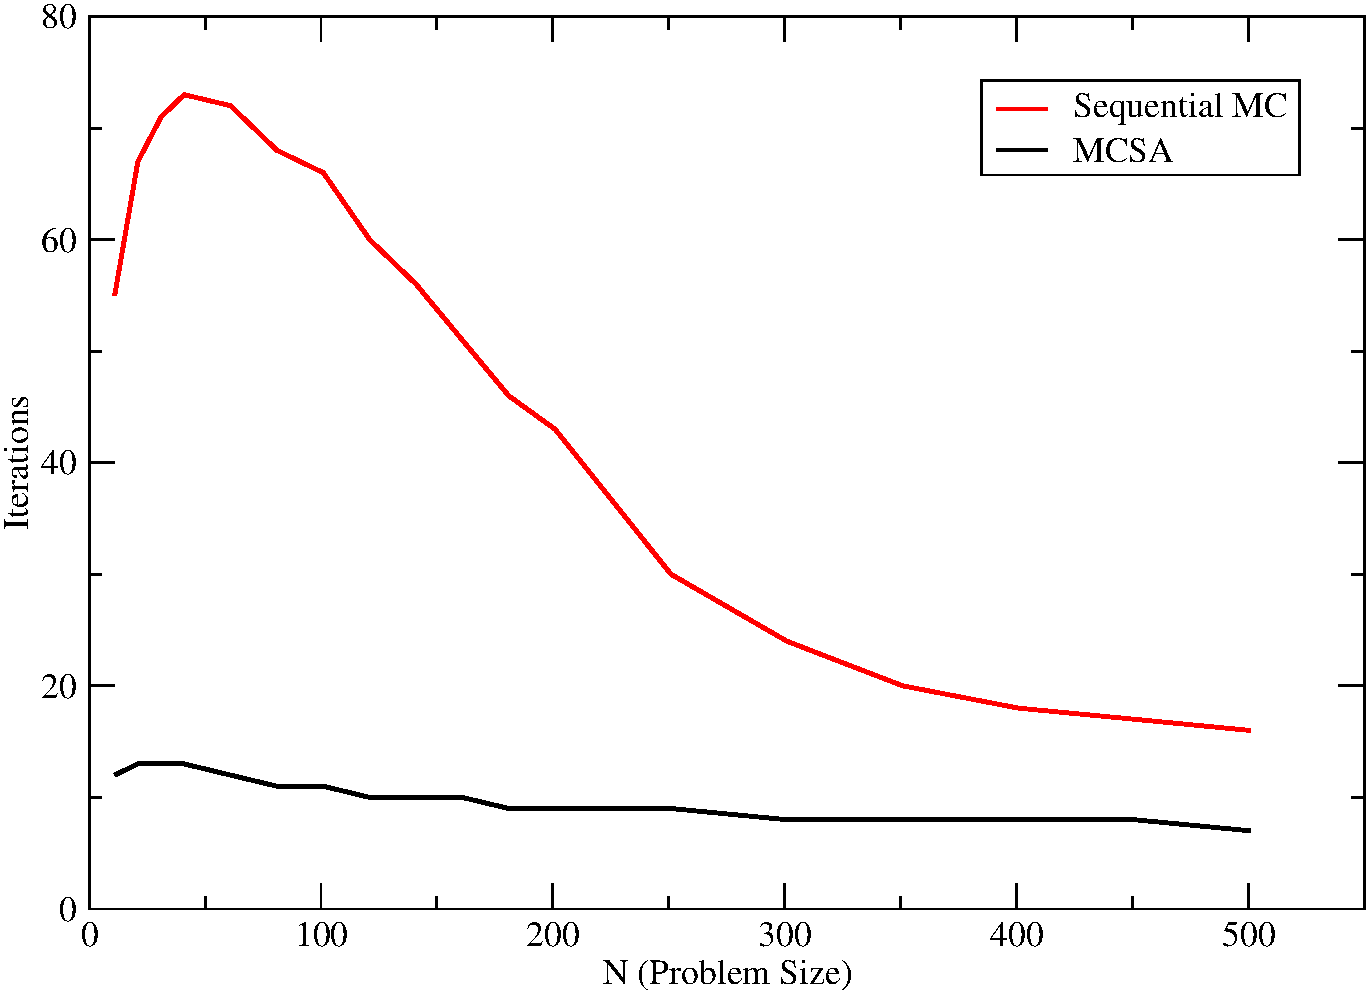
\includegraphics[width=4.5in,clip]{chapters/mc_background/seq_iterations.pdf}
  \caption{\textbf{Iterations to converge vs. Problem Size ($N$ for an
      $N \times N$ square mesh).} \textit{Both the Sequential Monte
      Carlo and MCSA solvers are used with the five point stencils and
      the adjoint Monte Carlo solver.}}
  \label{fig:seq_iterations}
\end{figure}

The benefits of using a synthetic acceleration scheme are also noted
when the infinity norm of the residual computed at each iteration for
both methods was collected at each iteration for a fixed problem sizes
of $N=100$ and $N=500$ as shown in figures Figure~\ref{fig:seq_100}
and \ref{fig:seq_500} respectively. In both cases, the Sequential
method is subject to two regimes of exponential convergence with high
frequency error modes removed in the first regime leaving lower
frequency and slower converging error modes in the second. Using MCSA
we a see a single rate of exponential convergence observed to be much
higher than that computed by Halton's method due to the fact that the
extra Richardson iteration is providing a smoothing effect to
alleviate the error mode variations. Even with the doubling of the
number of stochastic histories computed per time step in order to
ensure convergence for the Sequential method, we still see robustness
issues with a non-monotonically decreasing residual observed for the
$N=100$ case. In both cases the MCSA solver is observed to be robust
with a monotonically decreasing residual.

\begin{figure}[t!]
  \centering
  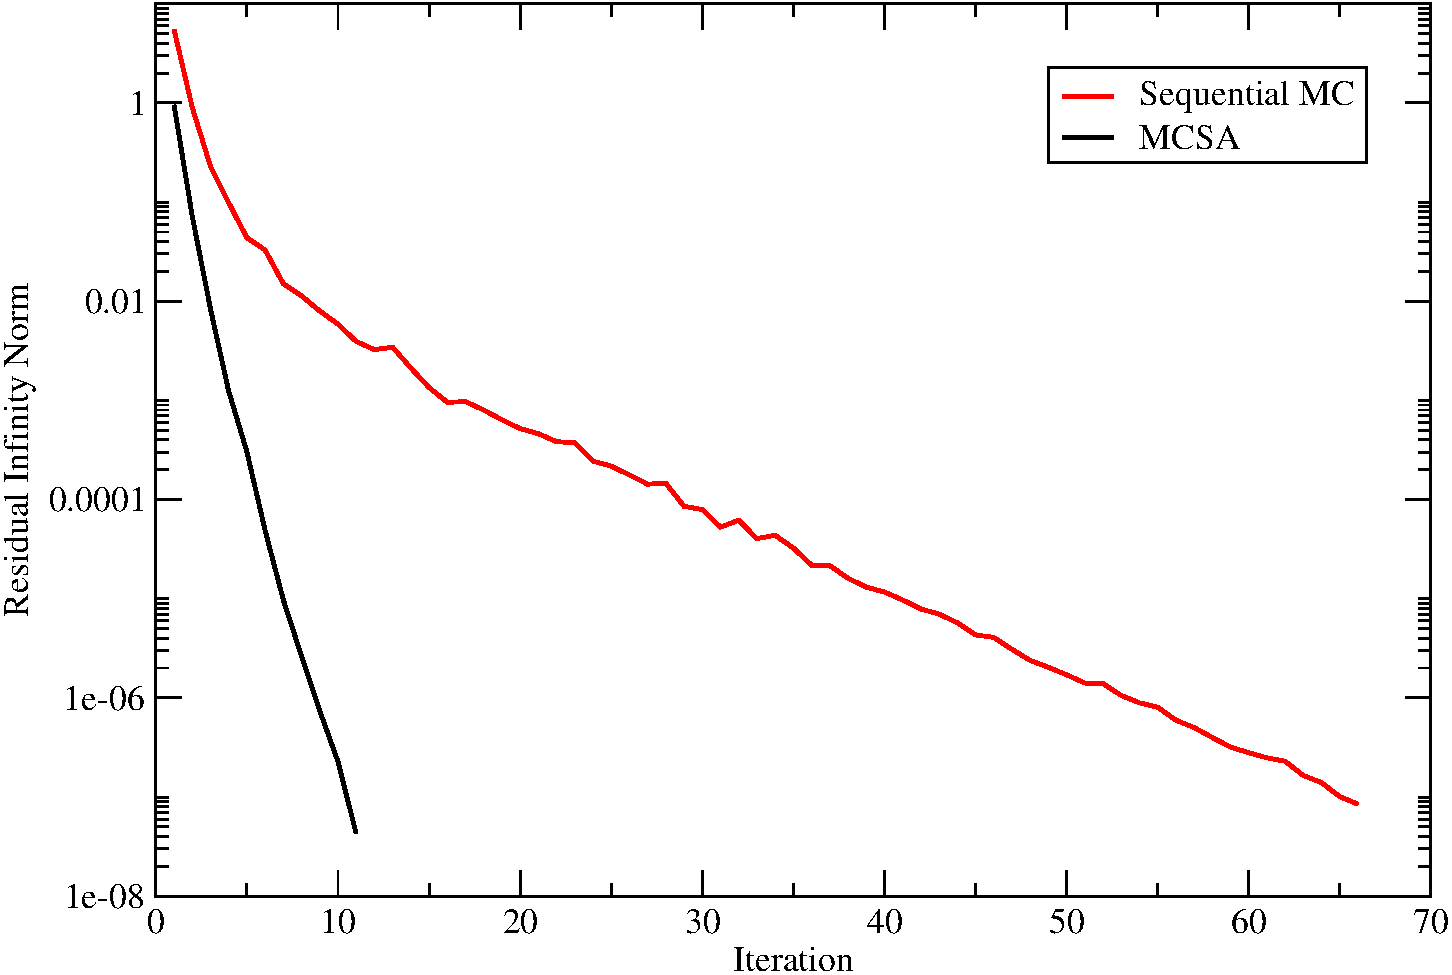
\includegraphics[width=4.5in,clip]{chapters/mc_background/seq_conv_100.pdf}
  \caption{\textbf{Infinity norm of the solution residual
      vs. iteration number for a problem of size $N=100$.}
    \textit{Both the Sequential Monte Carlo and MCSA solvers are used
      with the five point stencils and the adjoint Monte Carlo
      solver.}}
  \label{fig:seq_100}
\end{figure}

\begin{figure}[t!]
  \centering
  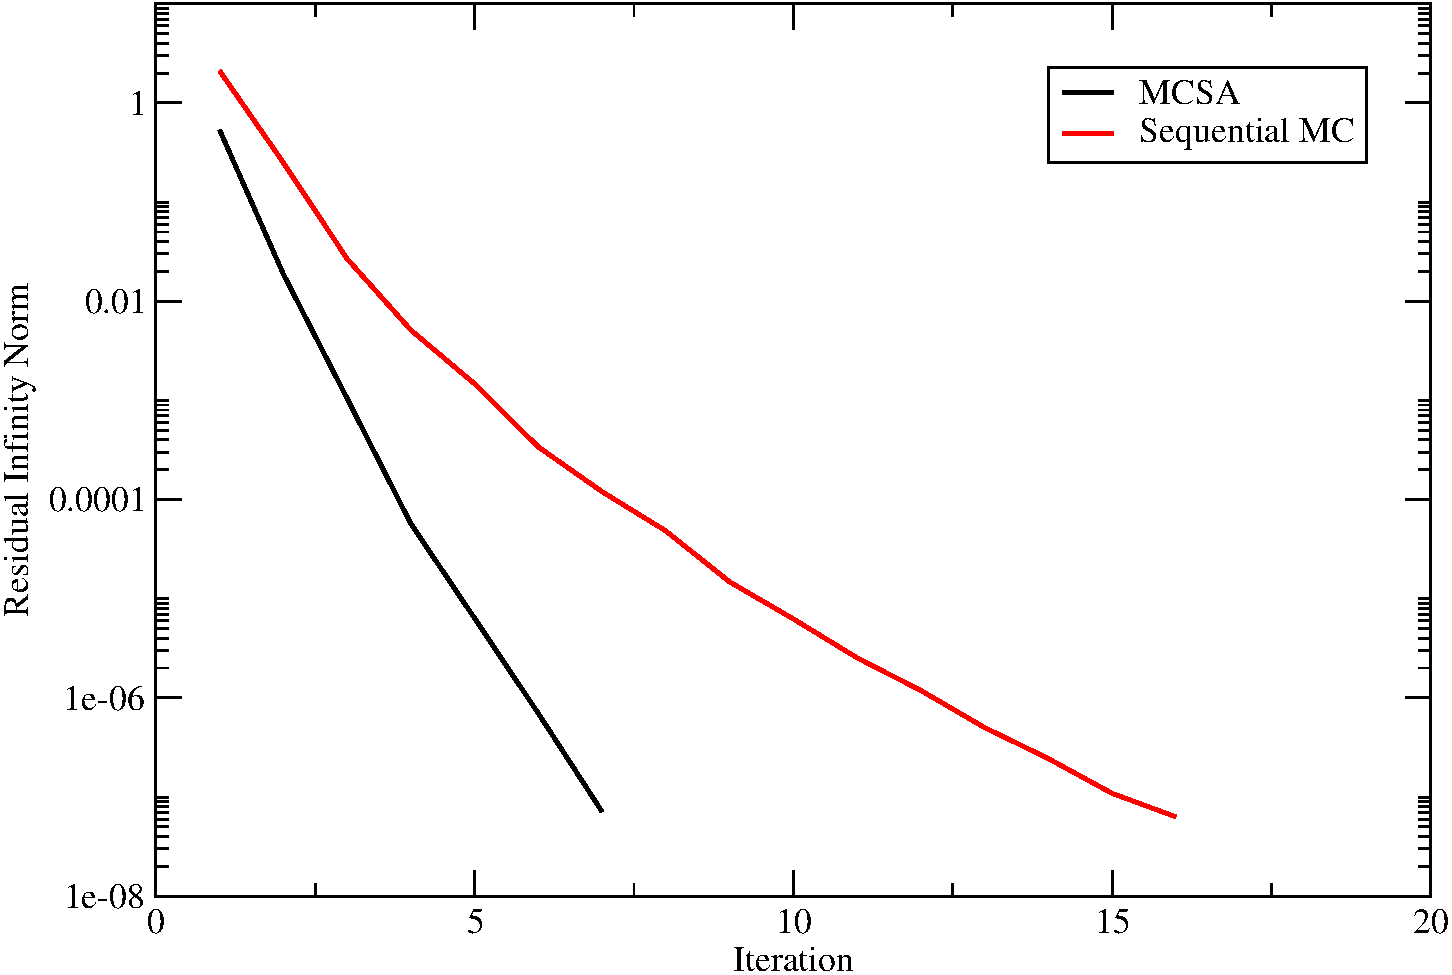
\includegraphics[width=4.5in,clip]{chapters/mc_background/seq_conv_500.pdf}
  \caption{\textbf{Infinity norm of the solution residual
      vs. iteration number for a problem of size $N=500$.}
    \textit{Both the Sequential Monte Carlo and MCSA solvers are used
      with the five point stencils and the adjoint Monte Carlo
      solver.}}
  \label{fig:seq_500}
\end{figure}

\clearpage

\subsection{Monte Carlo Parameter and Estimator Analysis}
\label{sec:parameter_estimator_analysis}
We now study the effects of the adjoint Monte Carlo parameters, weight
cutoff and number of histories, on MCSA performance with both the
collision and expected value estimators. With the same Poisson
problem, we will use a $200 \times 200$ grid and a convergence
tolerance of \sn{1}{-8} for all calculations. To study the effects of
the number of Monte Carlo histories per MCSA iteration, the weight
cutoff was fixed at \sn{1}{-4} while the number of histories per
iteration was varied from 6,000 to 100,000. It was observed that MCSA
would not converge for this problem using the collision estimator with
less than 6,000 histories while the expected value estimator permitted
convergence with only 2,000 histories.

Figure~\ref{fig:estimator_nh_iters} gives the number of iterations
required to converge for both estimators as a function of the number
of histories per iteration. For smaller numbers of histories, the
performance of the expected value estimator is significantly better
than the collision estimator. This result is valuable in that less
transport is required to achieve the same MCSA iterative performance
with the expected value estimator, important for situations where
transport is expensive (i.e. in domain decomposed
calculations). Interestingly, as the number of histories per iteration
are increased, the iterative performance with the collision estimator
approaches that of the expected value estimator. However, given the
performance of the expected value estimator at a fractional number of
histories, one should strongly consider its use over using the
collision estimator with more histories. The CPU time required to
converge is presented in Figure~\ref{fig:estimator_nh_time} and
reflects the results of the iterative performance. In general, using
the collision estimator is slightly slower overall, but the time per
iteration is faster due to the fact that the estimator does not have
to cycle through multiple states during the tally procedure.

\begin{figure}[t!]
  \centering
  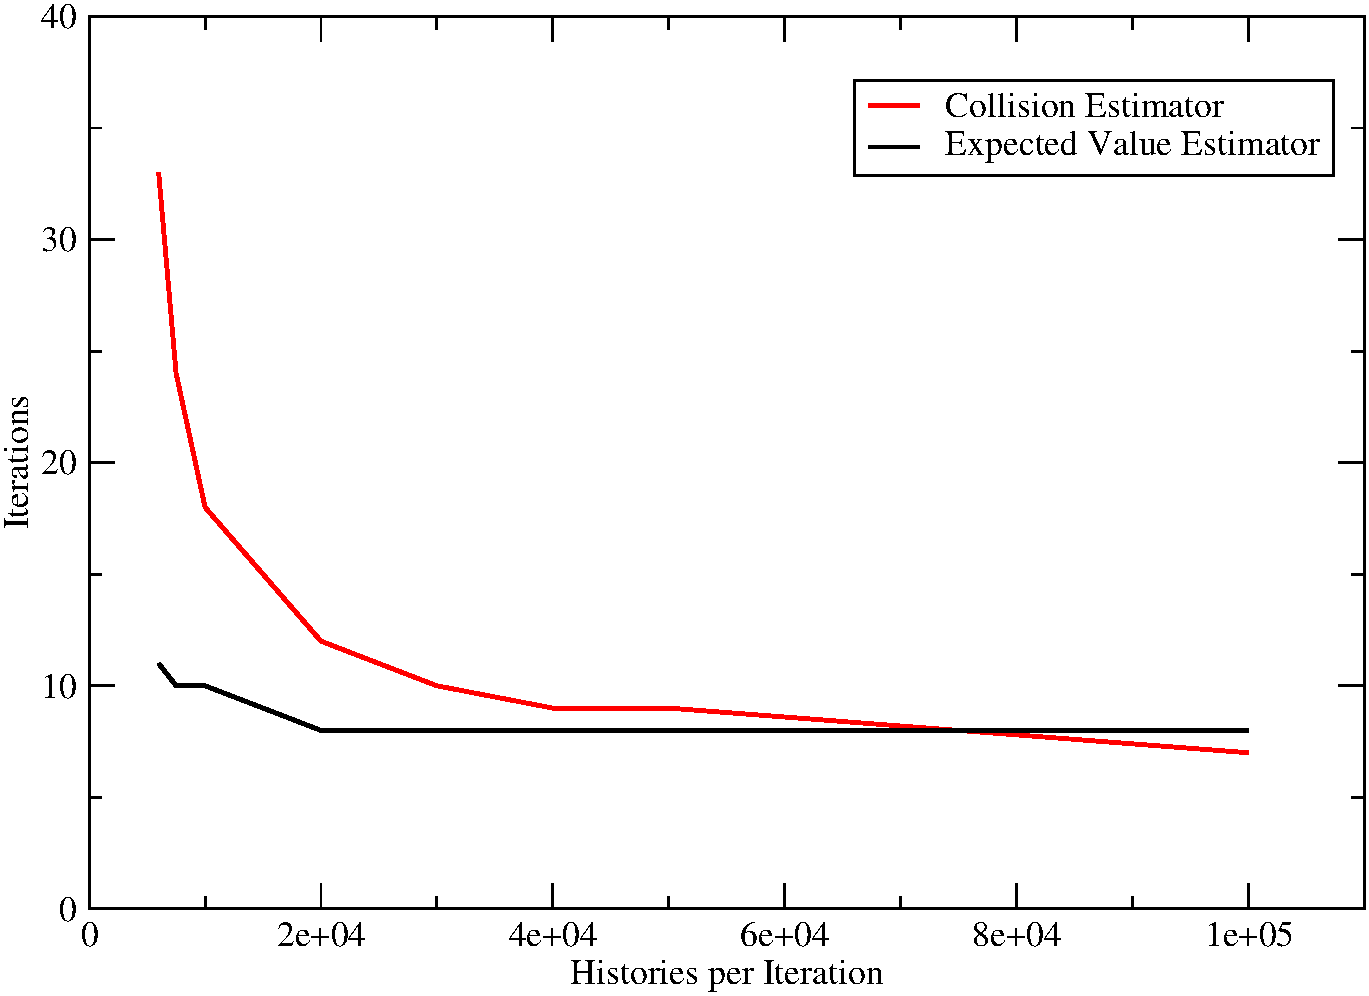
\includegraphics[width=4.75in,clip]{chapters/mc_background/estimator_nh_iters.pdf}
  \caption{\textbf{Iterations (s) to converge vs. Monte Carlo
      histories per MCSA iteration for a $200 \times 200$ square mesh
      and a weight cutoff of \sn{1}{-4}.} \textit{For low numbers of
      histories, the expected value estimator performance is
      significantly better than the collision estimator. At higher
      numbers of histories, the estimators become roughly
      equivalent.}}
  \label{fig:estimator_nh_iters}
\end{figure}

\begin{figure}[t!]
  \centering
  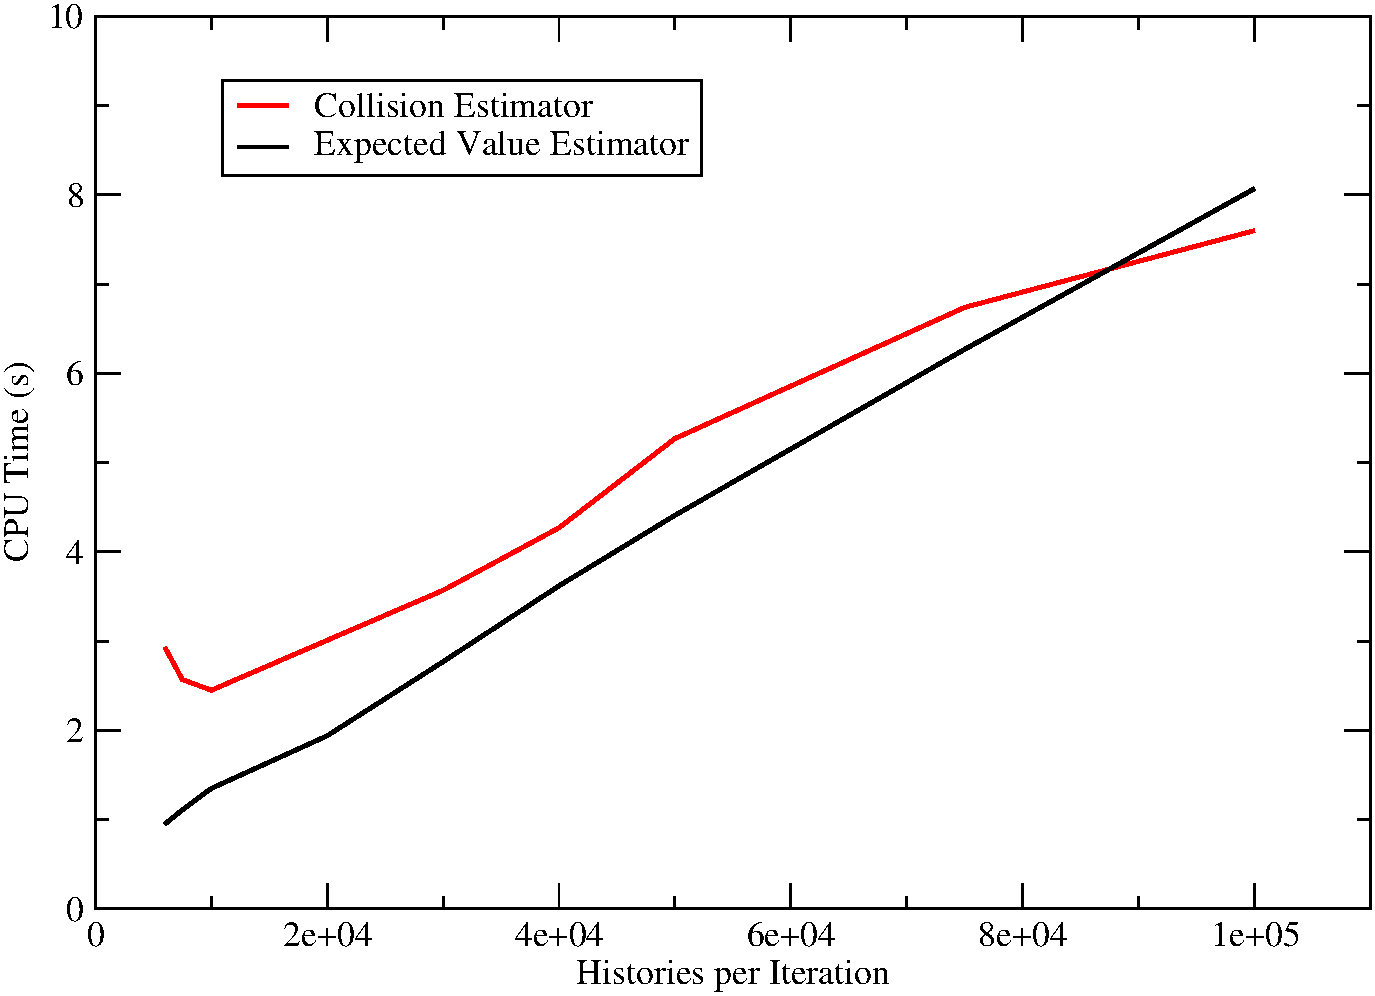
\includegraphics[width=4.75in,clip]{chapters/mc_background/estimator_nh_time.pdf}
  \caption{\textbf{CPU Time (s) to converge vs. Monte Carlo histories
      per MCSA iteration for a $200 \times 200$ square mesh and a
      weight cutoff of \sn{1}{-4}.} \textit{For low numbers of
      histories, the expected value estimator performance is better
      than the collision estimator due to a lower iteration count
      while the actual compute time per iteration is higher.}}
  \label{fig:estimator_nh_time}
\end{figure}

For the weight cutoff study, the number of histories per iteration was
fixed at 40,000 and the weight cutoff varied from \sn{5}{-1} down to
\sn{1}{-10}. Surprisingly, the number of iterations to converge given
by Figure~\ref{fig:estimator_wc_iters} is effectively invariant to the
weight cutoff, only seeing detrimental effects on the number of
iterations at a very large weight cutoff. This suggests that a fairly
large weight cutoff can be used in practice with both adjoint
estimators and that the preliminary components of the random walk are
more important to MCSA convergence than those that occur later and
with lower weight contributions. To further motivate using a larger
weight cutoff, Figure~\ref{fig:estimator_wc_time} gives the CPU time
need to converge as a function of weight cutoff. As expected, lowering
the weight cutoff lengthens the random walk lengths and increases CPU
time at no gain of iterative performance. In general, these results
suggest using the expected value estimator over the collision
estimator with MCSA as well as using a larger weight cutoff.

\begin{figure}[t!]
  \centering
  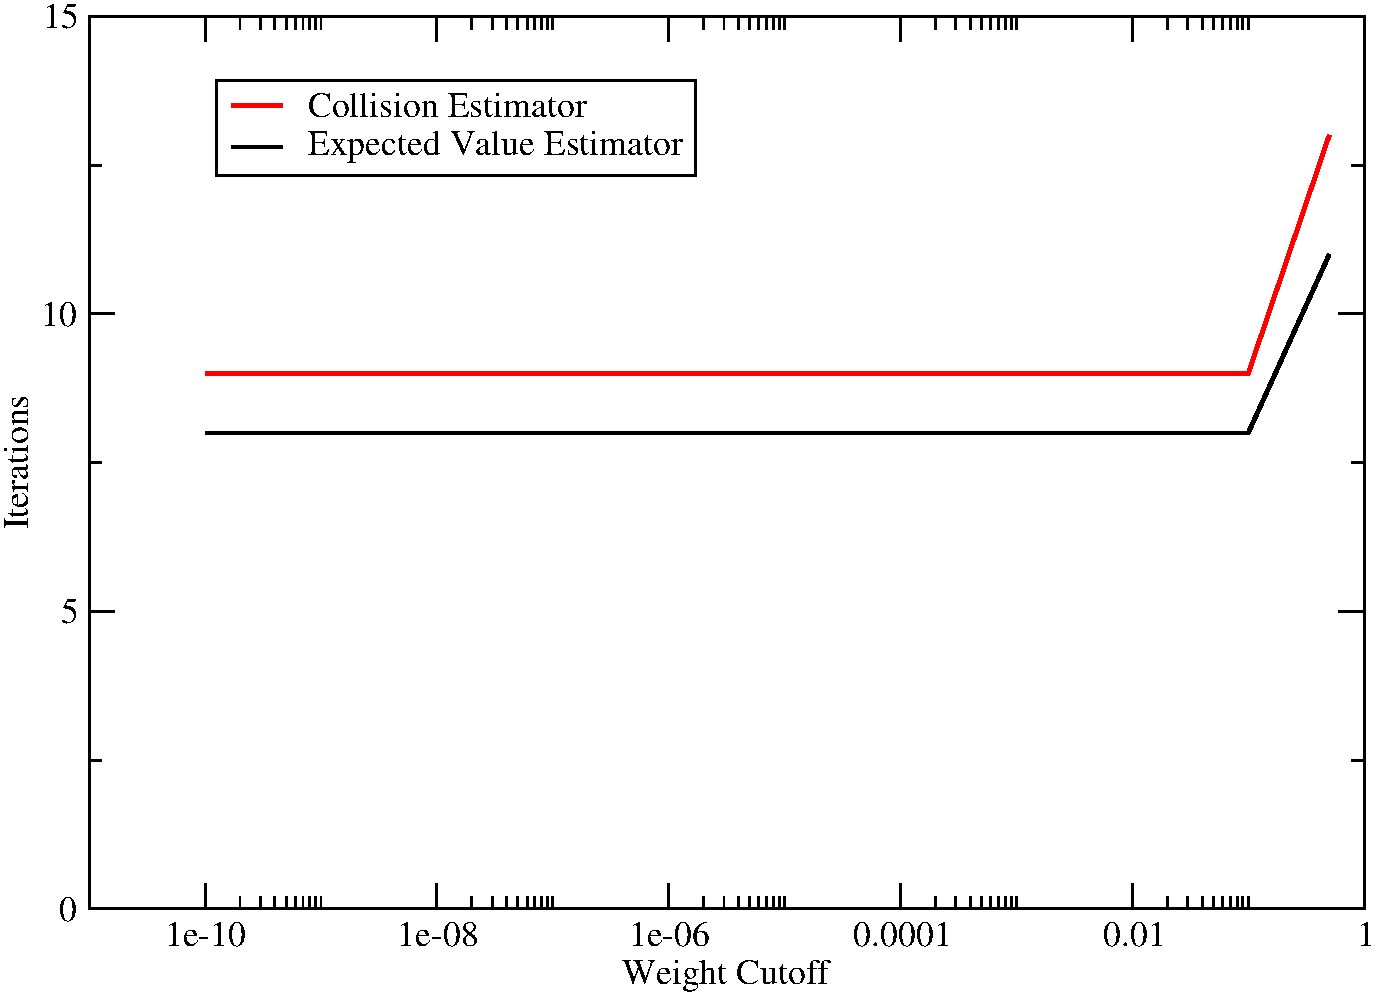
\includegraphics[width=4.75in,clip]{chapters/mc_background/estimator_wc_iters.pdf}
  \caption{\textbf{Iterations (s) to converge vs. history weight
      cutoff for a $200 \times 200$ square mesh and 40,000 histories.}
    \textit{For low numbers of histories, the expected value estimator
      performance is significantly better than the collision
      estimator. At higher numbers of histories, the estimators become
      roughly equivalent.}}
  \label{fig:estimator_wc_iters}
\end{figure}

\begin{figure}[t!]
  \centering
  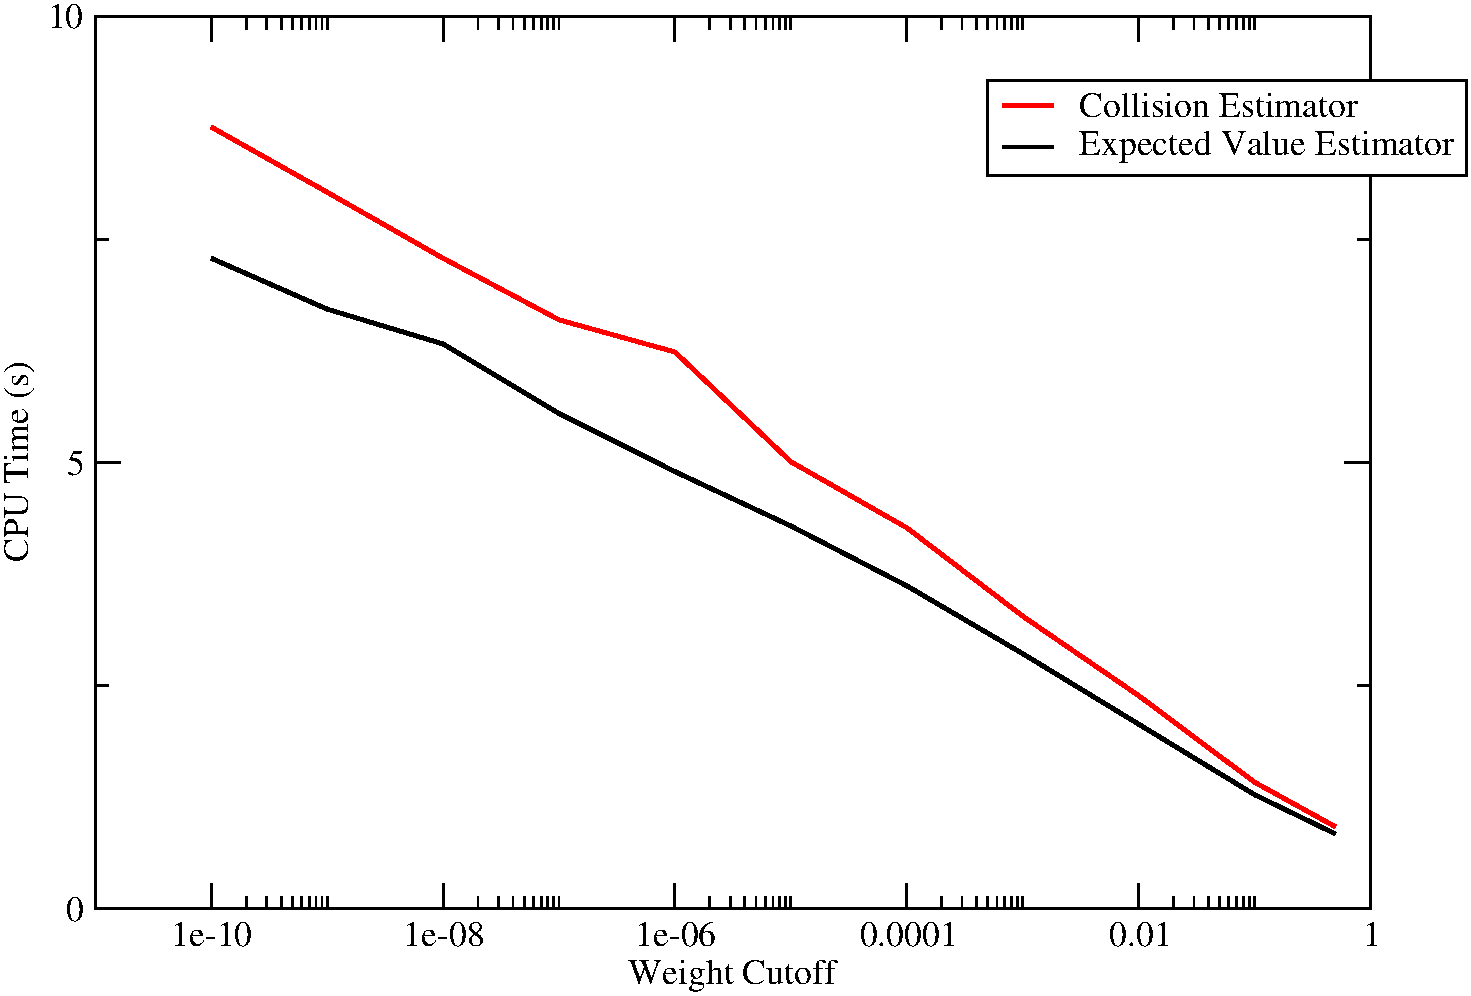
\includegraphics[width=4.75in,clip]{chapters/mc_background/estimator_wc_time.pdf}
  \caption{\textbf{CPU Time (s) to converge vs. history weight cutoff
      for a $200 \times 200$ square mesh and 40,000 histories.}
    \textit{For low numbers of histories, the expected value estimator
      performance is better than the collision estimator due to a
      lower iteration count while the actual compute time per
      iteration is higher.}}
  \label{fig:estimator_wc_time}
\end{figure}

\clearpage

%%---------------------------------------------------------------------------%%
\section{Summary}
\label{sec:mc_summary}

In this chapter, the fundamentals of Monte Carlo Synthetic
Acceleration methods were presented and explored in the context of a
simple model transport system. The following are the significant
observations, findings, and contributions.

\begin{itemize}
\item Monte Carlo Synthetic Acceleration (MCSA) has been generalized
  for all discrete linear transport problems
\item MCSA can be preconditioned using a general left/right scheme but
  requires the explicit inversion of the preconditioners and
  construction of the composite linear operator
\item The adjoint Neumann-Ulam method performs better when used with
  MCSA compared to the forward method
\item MCSA has superior performance when compared to Halton's residual
  Monte Carlo method
\item The Richardson iteration in MCSA behaves as a smoother for the
  stochastic Monte Carlo error
\item MCSA iterative performance when used with the expected value
  estimator is insensitive to histories per iteration
\item MCSA iterative performance is insensitive to the stochastic
  history weight cutoff
\end{itemize}

\blankpage
\chapter{Monte Carlo Solution Methods for the Simplified $P_N$ Equations}
\label{ch:mc_spn_solutions}

The neutron transport problem is complicated. Solutions cover a large
phase space and the problems of interest are often geometrically
complex, very large, or both, requiring tremendous computational
resources to generate an adequate solution. Modern deterministic
methods for large scale problems are commonly variants on the discrete
ordinates ($S_N$) method \cite{evans_denovo:_2010}. For full reactor
core neutronics simulations, the $S_N$ method requires potentially
trillions of unknown angular flux moments to be computed to achieve
good accuracy for the repsonses of interest. Other forms of the
transport problem, including the $P_N$ method, take on a simpler form
than the more common $S_N$ methods but lack in accuracy when compared
while still requiring considerable computational resources for
solutions in multiple dimensions.

In the 1960's, Gelbard developed an ad-hoc multidimensional extension
of the simple single dimension planar $P_N$ equations that created a
system of coupled, diffusion-like equations known as the simplified
$P_N$ ($SP_N$) equations. Up until around the 1990's, the $SP_N$
methods was either widely unknown, widely unused, or combination of
both even though numerical studies showed promising results with
better solutions than diffusion theory and a significant reduction in
computational time over more accurate methods such as discrete
ordinates. Why did this happen? A significant problem, pointed out by
Larsen, was that little rigor had been applied to the formulation of
the $SP_N$ equations since their derivation through primarily
heuristic arguments. Instead, studies at that time focused on simply
comparing the results of the method to other contemporary transport
solution strategies. In addition, many problems of interest from the
literature at the time were either solved using nodal-type methods for
reactor-sized problems or $S_N$-type methods for benchmark problems
with intricate material configurations and potentially large flux
gradients over small spatial domains.

So why reconsider the $SP_N$ equations? Starting in the 1990's and
primarily due to Larsen and his colleagues, the $SP_N$ equations have
been given a more rigorous treatment with both variational and
asymptotic derivations performed as a means of verification. In
addition, these equations have been more rigorously studied as
solution methods to MOX fuel problems and have been shown to provide
accurate solutions. With this mathematical literature to provide a
solid numerical footing for the method, we look at its application to
today's challenge problems in full reactor core transport. The
reduction in numerical complexity of current full core deterministic
solution methods using the $S_N$ approximation could mean significant
savings in both compute time and memory required. In addition, the
characteristics of the solution to the transport problem for a steady
state reactor core permit diffusion theory to be used; a staple of the
nuclear industry since its inception. Therefore, if diffusion theory
is applicable, then finer grained solutions that capture more of the
physics contained in the transport equation should be possible with
the $SP_N$ method. In doing so, we also expect from the literature to
obtain computed responses on the order of accuracy we would expect
from an appropriately discretized $S_N$ method at a fraction of the
cost. 

To further motivate moving in this direction, recent developments in
the Exnihilo neutronics package at Oak Ridge National Laboratory have
permitted generation of the $SP_N$ system of equations for detailed
full core reactor models. By fully forming these equations and
formulating them as a linear algebra problem, we now have access to
all of the modern advancements in computational linear algebra
including Krylov solvers for asymmetric systems and preconditioning
methods such as algebraic multigrid. This leads us to then explore the
applicability of our work in discrete Monte Carlo methods for linear
systems as a possible solution method for the $SP_N$ equations. If
formulated correctly, we hypothesize that signficant improvement in
usage of computational resources may be observed compared to modern
solution techniques such as those suggested. In addition, solving the
$SP_N$ equations in this way also breaks away from the $S_N$ forms of
parallelism where spatial parallelism is achieved by an efficient
parallel sweep, angular efficiency achieved by pipelining, and energy
parallelism achieved by decoupling the groups. With the $SP_N$
equations as a full matrix system, we now can parallelize the problem
as prescribed by the linear solver, which may be significantly more
scalable than current $S_N$ transport practices.

In this document we derive the multigroup $SP_N$ equations from the
Boltzmann transport equation. We then perform a spectral analysis on
the resulting system of equations to determine its potential
performance with both modern Krylov methods and Monte Carlo methods
for asymmetric linear systems. Following this, we devise a Monte Carlo
synthetic acceleration method as a proposed solution scheme.

%%---------------------------------------------------------------------------%%
\section{Derivation of the $SP_N$ Equations}
\label{sec:derivation}
In this section, we derive the $SP_N$ equations, closely following the
work of Evans. We begin by stating the general time-independent
neutron transport equation followed by a derivation of the $P_N$
equations in planar geometry for multiple energy groups. From these
equations, we then apply a set of approximations to yield the
multi-dimensional, multi-group $SP_N$ equations for fixed source
problems.

\subsection{The Neutron Transport Equation}
\label{subsec:transport_eq}
As a starting point we define the time-independent neutron transport
equation \cite{lewis_computational_1993}:
\begin{multline}
  \hat{\Omega} \cdot \vec{\nabla} \psi(\vec{r},\hat{\Omega},E) +
  \sigma(\vec{r},E) \psi(\vec{r},\hat{\Omega},E) = \\ \int \int
  \sigma_s(\vec{r},E' \rightarrow E,\hat{\Omega}' \rightarrow
  \hat{\Omega}) \psi(\vec{r},\hat{\Omega}',E') d\Omega' dE' +
  q(\vec{r},\hat{\Omega},E)\:,
  \label{eq:general_transport}
\end{multline}
with the variables defined as:
\begin{itemize}
\item $\vec{r}$ - neutron spatial position
\item $\hat{\Omega}$ - neutron streaming direction with radial
  component $\mu$ and azimuthal component $\omega$
\item $\hat{\Omega}' \cdot \hat{\Omega} = \mu_0$ is the angle of
  scattering
\item $E$ - neutron energy
\item $\psi(\vec{r},\hat{\Omega},E)$ - angular flux
\item $\sigma(\vec{r},E)$ - total interaction cross section
\item $\sigma_s(\vec{r},E' \rightarrow E,\hat{\Omega}')$ - probability
  of scattering from direction $\hat{\Omega}'$ into an angular domain
  $d\hat{\Omega}'$ about the direction $\hat{\Omega}$ and from energy
  $E'$ to an energy domain $dE'$ about energy $E$
\item $q(\vec{r},\hat{\Omega},E)$ - external source of neutrons.
\end{itemize}
For this work, it is sufficient to formulate
Eq~(\ref{eq:general_transport}) in 1-dimensonal Cartesian geometry:
\begin{multline}
  \mu \frac{\partial}{\partial x} \psi(x,\mu,E) + \sigma(x,E)
  \psi(x,\mu,E) = \\ \int \int \sigma_s(x,E') \rightarrow
  E,\hat{\Omega}' \rightarrow \hat{\Omega}) \psi(x,\hat{\Omega}',E')
  d\Omega' dE' + \frac{q(x,E)}{4 \pi}\:,
  \label{eq:cart_1d_transport}
\end{multline}
where the angular component of the solution is no longer dependent on
the azimuthal direction of travel and an isotropic source of neutrons
is assumed.

\subsection{Derivation of the $P_N$ Equations}
\label{subsec:pn_equations}
Next, we derive the $P_N$ equations, a simplified form of the general
transport equation where Legendre polynomials are used to expand the
angular flux and scattering cross section variables as a means of
capturing the angular structure of the solution. Before deriving this
form of the transport equation, we briefly discuss a few properties of
Legendre polynomials that we will find useful in the derivation.

\subsubsection{Legendre Polynomials}
\label{subsubsec:legendre_polys}
The Legendre polynomials are an orthogonal set of functions that
are solutions to Legendre's differential equation. They have the
following form \cite{lewis_computational_1993}:
\begin{equation}
  P_l(\mu) = \frac{1}{2^l l!}\frac{d^l}{d \mu^l}(\mu^2-1)^l\:.
  \label{eq:general_legendre_poly}
\end{equation}
These functions have several useful properties including
orthogonality:
\begin{equation}
  \int_{-1}^{1} P_l(\mu) P_{l'}(\mu) d\mu = \frac{1}{2l+1}\delta_{l l'}\:,
  \label{eq:legendre_orthog}
\end{equation}
a recurrence relation:
\begin{equation}
  \mu P_l(\mu) = \frac{1}{2l+1}[(l+1)P_{l+1}(\mu) + l P_{l-1}(\mu)]\:,
  \label{eq:legendre_recurrence}
\end{equation}
and an addition theorem:
\begin{equation}
  P_l(\hat{\Omega} \cdot \hat{\Omega}') = \frac{1}{2n+1}\sum_{m=-l}^l
  Y_{lm}(\hat{\Omega})Y^*_{lm}(\hat{\Omega}')\:,
  \label{eq:legendre_addition}
\end{equation}
where the functions $Y_{lm}(\hat{\Omega})$ are the spherical
harmonics. We can form the addition theorem in this way because the
spherical harmonics are in fact just harmonic multiples of the
Legendre polynomials:
\begin{equation}
  Y_{lm}(\hat{\Omega}) =
  \sqrt{\frac{(2l+1)(l-m)!}{(l+m)!}}P^m_l(\mu)e^{i \omega m}\:,
  \label{eq:spherical_harmonic}
\end{equation}
where $\omega$ is the azimuthal component of the streaming
direction. We can reduce Eq~(\ref{eq:legendre_addition}) for the
planar geometry we are studying by ignoring the azimuthal components
of the addition theorem. As shown in Eq~(\ref{eq:spherical_harmonic}),
the azimuthal dependence is given by the harmonic component, $e^{i
  \omega m}$, and therefore we choose to ignore all terms in
Eq.~(\ref{eq:legendre_addition}) where $m \neq 0$. This gives:
\begin{equation}
  P_l(\hat{\Omega} \cdot \hat{\Omega}') = \frac{1}{2n+1}
  Y_{l0}(\hat{\Omega})Y^*_{l0}(\hat{\Omega}')\:.
  \label{eq:legendre_addition_2}
\end{equation}
Per Eq~(\ref{eq:spherical_harmonic}) we have:
\begin{equation}
  Y_{l0}(\hat{\Omega}) = \sqrt{2l+1}P_l^0(\mu)\:,
  \label{eq:harmonic_0}
\end{equation}
where $P_l^0(\mu) = P_l(\mu)$ is the $0^{th}$ associated Legendre
function. Finally, we can reduce the addition theorem from
Eq~(\ref{eq:legendre_addition_2}) with Eq~(\ref{eq:harmonic_0}) to a
simple product for planar geometry:
\begin{equation}
  P_l(\hat{\Omega} \cdot \hat{\Omega}') = P_l(\mu)P_l(\mu')\:.
  \label{eq:legendre_addition_3}
\end{equation}

\subsubsection{Planar $P_N$ Equations}
\label{subsubsec:planar_pn}
With the Legendre polynomial properties defined above, we can proceed
by deriving the $P_N$ equations for planar geometry. For these
equations, we will start by assuming a monoenergtic field of neutrons
such that we are solving the following reduced form of the transport
equation: 
\begin{equation}
  \mu \frac{\partial}{\partial x} \psi(x,\mu) + \sigma(x) \psi(x,\mu)
  = \int d\Omega' \sigma_s(x,\hat{\Omega}' \rightarrow \hat{\Omega})
  \psi(\vec{r},\hat{\Omega}') + \frac{q(x)}{4 \pi}\:.
  \label{eq:mono_transport}
\end{equation}
The $P_N$ equations introduce the approximation that the angular
dependence of the scattering cross section, $\sigma_s$, and the angular
flux $\psi$, can be discretized by expanding them in Legendre
polynomials as follows:
\begin{equation}
  \psi(x,\mu) = \sum_{n=0}^\infty (2n+1)P_n(\mu)\phi_n(x)\:,
  \label{eq:flux_expansion}
\end{equation}
\begin{equation}
  \sigma_{sm}(x) = \sum_{m=0}^\infty (2m+1)P_m(\mu)\sigma_s(x)\:,
  \label{eq:scattering_expansion}
\end{equation}
where we have supressed the $2\pi$ generated by integrating away the
azimuthal angular component and $\phi_n(x)$ in
Eq~(\ref{eq:flux_expansion}) is referred to as the $n^{th}$ Legendre
moment of the neutron flux and is given by:
\begin{equation}
  \phi_n(x) = \int_{-1}^1 P_n(\mu)\psi(x,\mu)d\mu\:.
  \label{eq:legendre_moments}
\end{equation}
We first insert the expansions given by Eq~(\ref{eq:flux_expansion})
and (\ref{eq:scattering_expansion}) into the planar transport equation
given by Eq~(\ref{eq:mono_transport}):
\begin{multline}
  \frac{\partial}{\partial x}\Big[\sum_{n=0}^\infty (2n+1) \phi_n \mu
    P_n(\mu) \Big] + \sigma \sum_{n=0}^\infty (2n+1) \phi_n P_n(\mu) =
  \\ \int_{-1}^1 \sum_{m=0}^\infty (2m+1) \sigma_{sm} P_m(\mu_0)
  \sum_{n=0}^\infty (2n+1) \phi_n P_n(\mu') d \mu' + q\:,
  \label{eq:pn_deriv_1}
\end{multline}
where the dependence on the spatial variable, $x$, has been
supressed. To arrive at the $P_N$ equations we multiply
Eq~(\ref{eq:pn_deriv_1}) by $P_m(\mu)$ and integrate over the angular
domain $\int_{-1}^1 d \mu$. We will look at each term in
Eq~(\ref{eq:pn_deriv_1}) individually.

\paragraph{Streaming Term}
We first apply the multiplication and integration as prescribed above:
\begin{equation}
  \frac{\partial}{\partial x}\Bigg[\sum_{n=0}^\infty (2n+1) \mu \phi_n
    P_n(\mu) \Bigg] \rightarrow \int_{-1}^1 \frac{\partial}{\partial
    x}\Bigg[\sum_{n=0}^\infty (2n+1) \phi_n \mu P_n(\mu) P_m(\mu) \Bigg]
  d \mu\:.
  \label{eq:pn_deriv_2}
\end{equation}
The $\mu P_n(\mu)$ term can be eliminated via the recurrence relation
given by Eq~(\ref{eq:legendre_recurrence}):
\begin{equation}
\int_{-1}^1 \frac{\partial}{\partial x}\Bigg[\sum_{n=0}^\infty (2n+1)
  \frac{\phi_n}{2n+1}[(n+1)P_{n+1}(\mu) + n P_{n-1}(\mu)] P_m(\mu)
  \Bigg] d\mu\:,
\label{eq:pn_deriv_3}
\end{equation}
which expands to:
\begin{equation}
  \sum_{n=0}^\infty \frac{\partial}{\partial
    x}\phi_n\Bigg[(n+1)\int_{-1}^1 P_{n+1}(\mu)P_m(\mu) d\mu + n
    \int_{-1}^1 P_{n-1}(\mu) P_m(\mu) d\mu \Bigg] \:.
  \label{eq:pn_deriv_4}
\end{equation}
This reveals the orthogonality relation given by
Eq~(\ref{eq:legendre_orthog}) that when inserted into
Eq~(\ref{eq:pn_deriv_3}):
\begin{equation}
  \sum_{n=0}^\infty \frac{\partial}{\partial
    x}\phi_n\Bigg[(n+1)\frac{1}{2n+1}\delta_{n,n+1} +
    n\frac{1}{2n+1}\delta_{n,n-1} \Bigg] \:.
  \label{eq:pn_deriv_5}
\end{equation}
We can then distribute the Legendre moment to arrive at the final form
of the streaming term:
\begin{equation}
  \sum_{n=0}^\infty \frac{\partial}{\partial x} \frac{1}{2n+1} \Big[
    (n+1) \phi_{n+1} + n \phi_{n-1} \Big] \:.
  \label{eq:pn_deriv_6}
\end{equation}

\paragraph{Collision Term}
To reduce the collision term, the orthogonality relation is again
applied after the integration:
\begin{equation}
  \sigma \sum_{n=0}^\infty (2n+1) \phi_n P_n(\mu) \rightarrow
  \int_{-1}^1 \sigma \sum_{n=0}^\infty (2n+1) \phi_n P_n(\mu) P_m(\mu)
  d\mu\:,
  \label{eq:pn_deriv_7}
\end{equation}
\begin{equation}
  \sigma \sum_{n=0}^\infty (2n+1) \phi_n \frac{1}{2n+1}\:,
  \label{eq:pn_deriv_8}
\end{equation}
giving for the final collision term:
\begin{equation}
  \sum_{n=0}^\infty \sigma \phi_n \:.
  \label{eq:pn_deriv_9}
\end{equation}

\paragraph{Scattering Term}
For the scattering term:
\begin{multline}
  \int_{-1}^1 \sum_{m=0}^\infty (2m+1) \sigma_{sm} P_m(\mu_0)
  \sum_{n=0}^\infty (2n+1) \phi_n P_n(\mu') d\mu' \rightarrow\\
  \int_{-1}^1 \int_{-1}^1 \sum_{m=0}^\infty (2m+1) \sigma_{sm} P_m(\mu)
  P_m(\mu_0) \sum_{n=0}^\infty (2n+1) \phi_n P_n(\mu') d\mu' d\mu\:.
  \label{eq:pn_deriv_10}
\end{multline}
The addition thereom from Eq~(\ref{eq:legendre_addition_3}) is applied
to give:
\begin{equation}
  \int_{-1}^1 \int_{-1}^1 \sum_{m=0}^\infty (2m+1) \sigma_{sm} P_m(\mu)
  P_m(\mu)P_m(\mu') \sum_{n=0}^\infty (2n+1) \phi_n P_n(\mu') d\mu' d\mu\:,
  \label{eq:pn_deriv_11}
\end{equation}
which can be rearranged as:
\begin{equation}
  \sum_{m=0}^\infty \sum_{n=0}^\infty (2m+1) \sigma_{sm} (2n+1) \phi_n
  \int_{-1}^1 P_m(\mu') P_n(\mu') d\mu' \int_{-1}^1 P_m(\mu) P_m(\mu)
  d\mu\:.
  \label{eq:pn_deriv_12}
\end{equation}
Again we can apply orthogonality to eliminate the Legendre polynomials:
\begin{equation}
  \sum_{m=0}^\infty \sum_{n=0}^\infty (2m+1) \sigma_{sm} (2n+1) \phi_n
  \frac{1}{2n+1}\delta_{nm}\frac{1}{2m+1}\delta_{mm}\:,
  \label{eq:pn_deriv_13}
\end{equation}
which is reduced to:
\begin{equation}
  \sum_{n=0}^\infty \sigma_{sn} \phi_n\:,
  \label{eq:pn_deriv_14}
\end{equation}
with the dependence on the index $m$ eliminated.

\paragraph{Source Term}
The last term we are concerned with in Eq~(\ref{eq:pn_deriv_1}) is the
source term:
\begin{equation}
  q \rightarrow \int_{-1}^1 q P_n(\mu) d\mu \:.
  \label{eq:pn_deriv_15}
\end{equation}
We can leverage orthogonality by multiplying by $P_0(\mu) = 1$:
\begin{equation}
  \int_{-1}^1 q P_0 P_n(\mu) d\mu = \frac{q}{2*0+1}\delta_{n0}\:,
  \label{eq:pn_deriv_16}
\end{equation}
giving a final source term of:
\begin{equation}
  q\delta_{n0}\:.
  \label{eq:pn_deriv_17}
\end{equation}

Now that we have expanded all angular dependent terms in
Eq~(\ref{eq:pn_deriv_1}) and reduced them appropriately, we can
combine them to generate the $P_N$ equations:
\begin{equation}
    \sum_{n=0}^\infty \frac{\partial}{\partial x} \frac{1}{2n+1} \Big[
      (n+1) \phi_{n+1} + n \phi_{n-1} \Big] + \sum_{n=0}^\infty \sigma
    \phi_n = \sum_{n=0}^\infty \sigma_{sn} \phi_n + q\delta_{n0}\:.
  \label{eq:pn_deriv_18}
\end{equation}
More formally, the $P_N$ equations are written as:
\begin{equation}
   \frac{1}{2n+1} \frac{\partial}{\partial x}\Big[ (n+1) \phi_{n+1} + n
     \phi_{n-1} \Big] + \Sigma_n \phi_n = q\delta_{n0} \:,
  \label{eq:final_pn_equations}
\end{equation}
where $\Sigma_n = \sigma-\sigma_{sn}$ and the summations are truncated
at some level of approximation $N$ such that $n = 0,1,\dotsc,N$. This
yields a set of $N+1$ equations for $N+2$ flux moments. We therefore
require an additional equation to close the system. In accordance with
the series truncation as an approximation we choose the last moment in
the expansion to be zero:
\begin{equation}
  \phi_{N+1} = 0\:.
  \label{eq:pn_closure}
\end{equation}
As an example, we will construct the P5 equations from
Eq~(\ref{eq:final_pn_equations}) and the closure given by
Eq~(\ref{eq:pn_closure}):
\begin{subequations}
  \begin{gather}
   \frac{\partial}{\partial x}\phi_{1} + \Sigma_0 \phi_0 = q\:,\\ 
   \frac{1}{3} \frac{\partial}{\partial x}\Big[ 2
     \phi_{2} + \phi_{0} \Big] + \Sigma_1 \phi_1 = 0\:,\\
   \frac{1}{5} \frac{\partial}{\partial x}\Big[ 3 \phi_{3} + 2
     \phi_{1} \Big] + \Sigma_2 \phi_2 = 0 \:,\\
   \frac{1}{7} \frac{\partial}{\partial x}\Big[ 4 \phi_{4} + 3
     \phi_{2} \Big] + \Sigma_3 \phi_3 = 0 \:,\\
   \frac{1}{9} \frac{\partial}{\partial x}\Big[ 5 \phi_{5} + 4
     \phi_{3} \Big] + \Sigma_4 \phi_4 = 0 \:,\\
   \frac{1}{11} \frac{\partial}{\partial x} 5 \phi_{4} + \Sigma_5
   \phi_5 = 0 \:.
  \end{gather}
  \label{eq:p5_equations}
\end{subequations}
This gives us a set of 6 coupled equations for the six Legendre
moments requested defined over the entire spatial domain for a single
energy group. In practice, only odd-numbered $P_N$ orders are
generally used \cite{lewis_computational_1993}. This is due to the
fact that using odd $N$ yields an even number of $N+1$ equations which
can be split evenly on the left and right boundaries of the problem to
facilitate the description of boundary conditions. We will choose this
convention when deriving the boundary conditions.

\subsubsection{Boundary Conditions for the $P_N$ Equations}
\label{subsbusec:bcs_pn}
Per the analysis in \cite{lewis_computational_1993}, two types of
boundary conditions will be discussed: reflecting and Marshak. Marshak
boundary conditions can be used to specify both vacuum conditions and
isotropic source conditions on the boundary.

\paragraph{Reflecting Boundary Conditions}
In this case, the incoming flux should be equivalent to the outgoing
flux at the boundary point $x_b$:
\begin{equation}
  \psi(x_b,\mu) = \psi(x_b,-\mu)\:.
  \label{eq:reflecting_condition}
\end{equation}
Given the legendre expansion for the flux defined in
Eq~(\ref{eq:flux_expansion}) and the Legendre polynomial property that
$P_n(\mu) = (-1)^n P_n(-\mu)$, the condition specified by
Eq~(\ref{eq:reflecting_condition}) can be satisfied if
\begin{equation}
  \phi_n = 0,\ \forall \ \text{odd}\ n\:,
  \label{eq:reflecting_condition_odd}
\end{equation}
as all even $n$ yield $P_n(\mu) = P_n(-\mu)$ and therefore an
equivalent reflecting condition for the flux moments.

\paragraph{Marshak Boundary Conditions}
The Marshak conditions come directly from the Legendre moments of the
flux:
\begin{equation}
  \int_{\mu_b} P_i(\mu) \psi(\mu) d\mu = \int_{\mu_b} P_i(\mu)
  \psi_b(\mu) d\mu\ \ \ \ \ \ \ \ \ \ \text{for $i=1,3,...,N$}\:,
  \label{eq:general_marshak}
\end{equation}
where $\psi_b(\mu)$ is the prescribed angular flux on the boundary of
interest and $\mu_b$ the angular domain defined by the boundary. To
discretize this condition, we again insert the angular flux expansions
from Eq~(\ref{eq:flux_expansion}) for the fluxes defined in the
domain:
\begin{equation}
  \int_{\mu_b} P_i(\mu) \sum_{n=0}^N (2n+1) \phi_n P_n(\mu) d\mu =
  \int_{\mu_b} P_i(\mu) \psi_b(\mu) d\mu\:.
  \label{eq:marshak_expanded}
\end{equation}
The boundary flux, $\phi_b(\mu)$ is assumed to known and therefore
Eq~(\ref{eq:marshak_expanded}) defines a set of $(N+1)/2$ equations to
be solved on each boundary in the planar case, closing the system in
the spatial domain.

As an example of applying the Marshak conditions, consider the $P_3$
case with an isotropic boundary source $\phi_b$ on the left side of
the domain. In this case, the angular domain over which the boundary
flux is defined will be $\mu_b \in [0,1]$, giving the bounds of
integration. We first expand the summation for $i=1$:
\begin{equation}
  \int_0^1 \mu \Bigg[ \phi_0 + 3\phi_1\mu +
    \frac{5}{2}\phi_2(3\mu^2-1) + \frac{7}{2}\phi_3(5\mu^3-3\mu)
    \Bigg] d\mu = \int_0^1 \mu \phi_b d\mu\:,
  \label{eq:marshak_p1_deriv_1}
\end{equation}
and then $i=3$:
\begin{equation}
  \int_0^1 \frac{1}{2}(5\mu^3-3\mu) \Bigg[ \phi_0 + 3\phi_1\mu +
    \frac{5}{2}\phi_2(3\mu^2-1) + \frac{7}{2}\phi_3(5\mu^3-3\mu)
    \Bigg] d\mu = \int_0^1 \frac{1}{2}(5\mu^3-3\mu) \phi_b d\mu\:.
  \label{eq:marshak_p3_deriv_1}
\end{equation}
Expanding the polynomials in $\mu$ and carrying out the simple
integration then gives 2 equations for the left hand boundary:
\begin{equation}
  \phi_0 + 2\phi_1 + \frac{5}{4}\phi_2 = \phi_b\:,
  \label{eq:marshak_p1_deriv_2}
\end{equation}
\begin{equation}
  \phi_0 - 5\phi_2 - 8\phi_3 = \phi_b\:.
  \label{eq:marshak_p1_deriv_3}
\end{equation}
The right hand side boundary condition will yield 2 complementary
equations if Marshak conditions are used or 2 non-zero moments to be
solved for if reflected conditions are used. The formulation above
also holds for vacuum conditions where $\phi_b = 0$.

\subsection{Formulation of the $SP_N$ Equations}
\label{subsec:spn_equations}
The $P_N$ equations give $N+1$ coupled first-order equations
capturing the spatial and angular-dependence of the solution. In
multiple dimensions, the equation set becomes large and coupled not
only through angular moments but also through the spatial
variables. As a simpler alternative to multidimensional $P_N$
solutions, Gelbard recognized in 1960 that the planar $P_N$ equations
could be simplified and applied an ad-hoc method to extend them to
multiple dimensions, yielding the $SP_N$ equations. These equations
are not only fewer in number, but also take on a diffusion-like form
while maintaining the angular character of the flux, making them
amenable to solutions with modern diffusion methods.

First, the $P_N$ equations can be simplified to $(N+1)/2$ second-order
equations by solving for the $n^th$ Legendre flux moment in the
odd-order equations:
\begin{equation}
  \phi_n = \frac{1}{\Sigma_n}\Bigg[ q \delta_{no} -
    \frac{\partial}{\partial x}\Big(\frac{n}{2n+1}\phi_{n-1} +
    \frac{n+1}{2n+1} \phi_{n+1} \Big) \Bigg]\:, 
  \label{eq:odd_moments}
\end{equation}
for $n = 1,3,\cdots,N$ and $\delta_{no} = 0\ \forall n \neq 0$. We can
insert the odd moments into Eq~(\ref{eq:final_pn_equations}) to get a
reduced group of equations for the even moments:
\begin{multline}
  -\frac{\partial}{\partial x}
  \Bigg[\frac{n}{2n+1}\frac{1}{\Sigma_{n-1}} \frac{\partial}{\partial
      x} \Big(\frac{n-1}{2n-1} \phi_{n-2} + \frac{n}{2n-1}\phi_n \Big)
    \\+ \frac{n+1}{2n+1}\frac{1}{\Sigma_{n+1}} \frac{\partial}{\partial
      x} \Big(\frac{n+1}{2n+3}\phi_n + \frac{n+2}{2n+3}\phi_{n+2}\Big)
    \Bigg] \\+ \Sigma_n \phi_n = q \delta_{n0}\ \ \ \ \ \ \ \ \ n =
  0,2,4,\cdots,N\:.
  \label{eq:reduced_pn}
\end{multline}
Immediately, we note the diffusion-like nature of
Eq~(\ref{eq:reduced_pn}) as compared to the original $P_N$
equations. To extend these equations to multiple dimensions, gelbard
simple replaced the x-plane spatial derivatives in the reduced set of
equations with general multidimensional gradient operators:
\begin{multline}
  -\nabla \cdot \Bigg[\frac{n}{2n+1}\frac{1}{\Sigma_{n-1}} \nabla
    \Big(\frac{n-1}{2n-1} \phi_{n-2} + \frac{n}{2n-1}\phi_n \Big) \\+
    \frac{n+1}{2n+1}\frac{1}{\Sigma_{n+1}} \nabla
    \Big(\frac{n+1}{2n+3}\phi_n + \frac{n+2}{2n+3}\phi_{n+2}\Big)
    \Bigg] \\+ \Sigma_n \phi_n = q \delta_{n0}\ \ \ \ \ \ \ \ \ n =
  0,2,4,\cdots,N\:,
  \label{eq:spn_equations}
\end{multline}
yielding a multidimensional set of $(N+1)/1$ angular coupled equations
known as the $SP_N$. Again, we provide closure to this set of
equations with $\phi_{N+1} = 0$. As a concrete example, we will
consider the $SP_7$ equations:
\begin{subequations}
  \begin{gather}
    -\nabla \cdot \frac{1}{3 \Sigma_1} \nabla ( \phi_0 + 2\phi_2 ) +
    \Sigma_0 \phi_0 = q \\ 
    -\nabla \cdot \Bigg[ \frac{2}{15 \Sigma_1} \nabla ( \phi_0 + 2\phi_2
      ) + \frac{3}{35 \Sigma_3}\nabla( 3\phi_2 + 4\phi_4)\Bigg] +
    \Sigma_2 \phi_2 = 0\\
    -\nabla \cdot \Bigg[ \frac{4}{63 \Sigma_3} \nabla ( 3\phi_2 +
      4\phi_4 ) + \frac{5}{99 \Sigma_5}\nabla( 5\phi_4 +
      6\phi_6)\Bigg] + \Sigma_4 \phi_4 = 0\\
    -\nabla \cdot \Bigg[ \frac{6}{143 \Sigma_5} \nabla ( 5\phi_4 +
      6\phi_6 ) + \frac{7}{195 \Sigma_7}\nabla(7\phi_6)\Bigg] +
    \Sigma_6 \phi_6 = 0 \:.
  \end{gather}
  \label{eq:sp7_equations}
\end{subequations}
To further modify these equations, we can use a change of variables to
create a new group of equations such that the gradients are operating
on a single vector:
\begin{subequations}
  \begin{gather}
    u_1 = \phi_0 + 2\phi_2 \\
    u_2 = 3\phi_2 + 4\phi_4 \\
    u_3 = 5\phi_4 + 6\phi_6 \\
    u_4 = 7\phi_6 \:,
  \end{gather}
  \label{eq:spn7_subs}
\end{subequations}
or equivalently:
\begin{subequations}
  \begin{gather}
    \phi_0 = u_1 - \frac{2}{3}u_2 + \frac{8}{15}u_3 -
    \frac{16}{35}u_4 \\
    \phi_2 = \frac{1}{3}u_2 - \frac{4}{15}u_3 + \frac{8}{35}u_4\\ 
    \phi_4 = \frac{1}{5}u_3 - \frac{6}{35}u_4\\
    \phi_6 = \frac{1}{7}u_4\:.
  \end{gather}
  \label{eq:spn7_subs_inverse}
\end{subequations}
When substituted into Eq~(\ref{eq:sp7_equations}), these terms give:
\begin{subequations}
  \begin{gather}
    -\nabla \cdot \frac{1}{3 \Sigma_1} \nabla u_1 + \Sigma_0 \Bigg[
    u_1 - \frac{2}{3}u_2 + \frac{8}{15}u_3 - \frac{16}{35}u_4 \Bigg]
    = -q \\
    -\nabla \cdot \Bigg[ \frac{2}{15 \Sigma_1} \nabla u_1 +
    \frac{3}{35 \Sigma_3} \nabla u_2 \Bigg] + \Sigma_2 \Bigg[
    \frac{1}{3}u_2 - \frac{4}{15}u_3 + \frac{8}{35}u_4 \Bigg] = 0 \\
    -\nabla \cdot \Bigg[ \frac{4}{63 \Sigma_3} \nabla u_2 +
    \frac{5}{99 \Sigma_5} \nabla u_3 \Bigg] + \Sigma_4 \Bigg[
    \frac{1}{5}u_3 - \frac{6}{35}u_4 \Bigg] = 0 \\ 
    -\nabla \cdot \Bigg[ \frac{6}{143 \Sigma_5} \nabla u_3 +
    \frac{7}{195 \Sigma_7} \nabla u_4 \Bigg] + \Sigma_6 \Bigg[
    \frac{1}{7}u_4 \Bigg] = 0 \:.
  \end{gather}
  \label{eq:spn7_subs_equations}
\end{subequations}
If we rearrange the Eq~(\ref{eq:spn7_subs_equations} such that only
one divergence operation is present in each equation, we can formulate
this as a matrix system of 4 equations in the case of the $SP_7$
approximation:
\begin{equation}
  -\nabla \cdot D_n \nabla u_n + \sum_{m=1}^4 A_{nm} u_m =
  q_n\ \ \ \ \ \ \ n = 1,2,3,4\:,
  \label{eq:spn_matrix}
\end{equation}
with $\mathbf{u}$ the vector of solution variables:
\begin{equation}
  \mathbf{u} = ( u_1\ \ u_2\ \ u_3\ \ u_4 )^T \:,
  \label{eq:spn7_solution_vector}
\end{equation}
$\mathbf{D}$ the vector of effective diffusion coefficients:
\begin{equation}
  \mathbf{D} = \Bigg( \frac{1}{3\Sigma_1}\ \ \frac{1}{7\Sigma_3}\ \
  \frac{1}{11\Sigma_5}\ \ \frac{1}{15\Sigma_7} \Bigg)^T\:,
  \label{eq:spn7_diffusion_coeffs}
\end{equation}
$\mathbf{q}$ the vector of source terms where the $0^{th}$ moment
source has now been distributed through the system:
\begin{equation}
  \mathbf{q} = (
  q\ \ -\frac{2}{3}q\ \ \frac{8}{15}q\ \ -\frac{16}{35}q )^T\:,
  \label{eq:spn7_source_vector}
\end{equation}
and $\mathbf{A}$ a matrix of angular scattering terms:
% NOTE: I copied the following matrix directly out of Tom's tech note
% on the SPn equations which I am effectively following here because I
% was feeling lazy. I have verified its correctness.
\begin{equation}
  \mathbf{A} = 
  \begin{bmatrix}
    (\Sigma_0) &
    (-\frac{2}{3}\Sigma_0) &
    (\frac{8}{15}\Sigma_0) &
    (-\frac{16}{35}\Sigma_0) \\
    %%
    &&&\\
    %%
    (-\frac{2}{3}\Sigma_0) &
    (\frac{4}{15}\Sigma_0 + \frac{1}{3}\Sigma_2) &
    (-\frac{16}{45}\Sigma_0 - \frac{4}{9}\Sigma_2) &
    (\frac{32}{105}\Sigma_0 + \frac{8}{21}\Sigma_2) \\
    %%
    &&&\\
    %%
    (\frac{8}{15}\Sigma_0) &
    (-\frac{16}{45}\Sigma_0 - \frac{4}{9}\Sigma_2) &
    (\frac{64}{225}\Sigma_0 + \frac{16}{45}\Sigma_2 + \frac{9}{25}\Sigma_4) &
    (-\frac{128}{525}\Sigma_0 - \frac{32}{105}\Sigma_2 - \frac{54}{175}\Sigma_4)
    \\ 
    %%
    &&&\\
    %%
    (-\frac{16}{35}\Sigma_0) &
    (\frac{32}{105}\Sigma_0 + \frac{8}{21}\Sigma_2) &
    (-\frac{128}{525}\Sigma_0 - \frac{32}{105}\Sigma_2 - \frac{54}{175}\Sigma_4)
    & 
    (\frac{256}{1225}\Sigma_0 + \frac{64}{245}\Sigma_2 +
    \frac{324}{1225}\Sigma_4 + \frac{13}{49}\Sigma_6)
  \end{bmatrix}\:.
  \label{eq:A_matrix}
\end{equation}
Note that the term $\sum_{m=1}^4 A_{nm} u_m$ in
Eq~(\ref{eq:spn_matrix}) couples the moments in each equation while
the diffusive term in each equation is only for a single
'psuedo-moment' $u_n$. This completes the derivation of the $SP_7$
equations for a single energy group. As noted by Evans, lower order
$SP_N$ approximations can be generated by setting higher order even
moments in this system to zero (e.g. $\phi_6 = \phi_4 = 0$ yields the
$SP_3$ equations).

\subsubsection{Boundary Conditions for the $SP_N$ Equations}
\label{subsubsec:spn_boundary_conditions}
We approach the formulation of the boundary conditions in much the
same way as we did for the $P_N$ equations with both reflecting and
Marshak conditions possible. To begin, we perform the expansion in
Eq~(\ref{eq:marshak_expanded}) for the left side of the planar system,
this time for $N=7$ to correspond to our $SP_7$ system. For $i=1$:
\begin{multline}
  \int_0^1 \mu \Bigg[ \phi_0 + 3\phi_1\mu +
    \frac{5}{2}\phi_2(3\mu^2-1) + \frac{7}{2}\phi_3(5\mu^3-3\mu)
    +\\ \frac{1}{8}(63\mu^5-70\mu^3+15\mu) \Bigg] d\mu = \int_0^1 \mu
  \phi_b d\mu\:,
  \label{eq:spn_bnd_p1}
\end{multline}
for $i=3$,
\begin{multline}
  \int_0^1 \frac{1}{2}(5\mu^3-3\mu) \Bigg[ \phi_0 + 3\phi_1\mu +
    \frac{5}{2}\phi_2(3\mu^2-1) + \frac{7}{2}\phi_3(5\mu^3-3\mu) +\\
    \frac{1}{8}(63\mu^5-70\mu^3+15\mu) \Bigg] d\mu = \int_0^1
  \frac{1}{2}(5\mu^3-3\mu) \phi_b d\mu\:,
  \label{eq:spn_bnd_p3}
\end{multline}
for $i=5$:
\begin{multline}
  \int_0^1 \frac{1}{8}(63\mu^5-70\mu^3+15\mu) \Bigg[ \phi_0 + 3\phi_1\mu +
    \frac{5}{2}\phi_2(3\mu^2-1) + \frac{7}{2}\phi_3(5\mu^3-3\mu) +\\
    \frac{1}{8}(63\mu^5-70\mu^3+15\mu) \Bigg] d\mu = \int_0^1
  \frac{1}{8}(63\mu^5-70\mu^3+15\mu) \phi_b d\mu\:,
  \label{eq:spn_bnd_p5}
\end{multline}
and for $i=7$:
\begin{multline}
  \int_0^1 \frac{1}{16}(429\mu^7-693\mu^5+315\mu^3+35\mu) \Bigg[
    \phi_0 + 3\phi_1\mu + \frac{5}{2}\phi_2(3\mu^2-1) +
    \frac{7}{2}\phi_3(5\mu^3-3\mu) \\+
    \frac{1}{8}(63\mu^5-70\mu^3+15\mu) +
    \frac{1}{16}(429\mu^7-693\mu^5+315\mu^3+35\mu) \Bigg] d\mu =\\
  \int_0^1 \frac{1}{16}(429\mu^7-693\mu^5+315\mu^3+35\mu) \phi_b
  d\mu\:.
  \label{eq:spn_bnd_p7}
\end{multline}
Carrying out the simple integrations yields the following system of
equations:
\begin{subequations}
  \begin{gather}
    \frac{1}{2}\phi_0 + \phi_1 + \frac{5}{8}\phi_2 -
    \frac{3}{16}\phi_4 + \frac{13}{128}\phi_6 =
    \frac{1}{2}\phi_{b}\\ -\frac{1}{8}\phi_0 + \frac{5}{8}\phi_2 +
    \phi_3 + \frac{81}{128}\phi_4 - \frac{13}{64}\phi_6 =
    -\frac{1}{8}\phi_{b}\\ \frac{1}{16}\phi_0 - \frac{25}{128}\phi_2 +
    \frac{81}{128}\phi_4 + \phi_5 + \frac{325}{512}\phi_6 =
    \frac{1}{16}\phi_{b}\\ -\frac{5}{128}\phi_0 + \frac{7}{64}\phi_2 -
    \frac{105}{512}\phi_4 + \frac{325}{512}\phi_6 + \phi_7 =
    -\frac{5}{128}\phi_{b}\:,
  \end{gather}
  \label{eq:spn_bnd_integrated}
\end{subequations}
where $\phi_b$ is again an isotropic source prescribed on the planar
boundary. For the odd moment in each boundary equation, we insert
Eq~(\ref{eq:odd_moments}) to remove them, leaving only the even
moments and a set of differential equations:
\begin{subequations}
  \begin{gather}
    \frac{1}{2}\phi_0 + \frac{1}{3\Sigma_1}\frac{\partial}{\partial
      x}(\phi_0+2\phi_2) + \frac{5}{8}\phi_2 - \frac{3}{16}\phi_4 +
    \frac{13}{128}\phi_6 = \frac{1}{2}\phi_{b}\\ -\frac{1}{8}\phi_0 +
    \frac{5}{8}\phi_2 + \frac{1}{7\Sigma_3}\frac{\partial}{\partial
      x}(3\phi_2 + 4\phi_4) + \frac{81}{128}\phi_4 -
    \frac{13}{64}\phi_6 = -\frac{1}{8}\phi_{b}\\ \frac{1}{16}\phi_0 -
    \frac{25}{128}\phi_2 + \frac{81}{128}\phi_4 +
    \frac{1}{11\Sigma_5}\frac{\partial}{\partial x}(5\phi_4 + 6\phi_6)
    + \frac{325}{512}\phi_6 =
    \frac{1}{16}\phi_{b}\\ -\frac{5}{128}\phi_0 + \frac{7}{64}\phi_2 -
    \frac{105}{512}\phi_4 + \frac{325}{512}\phi_6 +
    \frac{1}{15\Sigma_7}\frac{\partial}{\partial x}(7\phi_6)
    = -\frac{5}{128}\phi_{b}\:.
  \end{gather}
  \label{eq:spn_bnd_subs}
\end{subequations}
We can again make the substitution of variables given by
Eqs~(\ref{eq:spn7_subs}) and (\ref{eq:spn7_subs_inverse}) for
consitency with the equations defined on the domain. In addition, we
apply the $SP_N$ approximation to the derivatives by assuming they are
instead multidimensional gradients on the boundary such that
$\frac{\partial}{\partial x} \rightarrow
\hat{\mathbf{n}}\cdot\nabla$. Doing this gives:
\begin{multline}
    \frac{1}{2}\Big(u_1 - \frac{2}{3}u_2 + \frac{8}{15}u_3 -
    \frac{16}{35}u_4\Big) +
    \frac{1}{3\Sigma_1}\hat{\mathbf{n}}\cdot\nabla\Big(\Big(u_1 -
    \frac{2}{3}u_2 + \frac{8}{15}u_3 -
    \frac{16}{35}u_4\Big)+\\2\Big(\frac{1}{3}u_2 - \frac{4}{15}u_3 +
    \frac{8}{35}u_4\Big)\Big) + \frac{5}{8}\Big(\frac{1}{3}u_2 -
    \frac{4}{15}u_3 + \frac{8}{35}u_4\Big)
    -\\ \frac{3}{16}\Big(\frac{1}{5}u_3 - \frac{6}{35}u_4\Big) +
    \frac{13}{128}\Big(\frac{1}{7}u_4\Big) = \frac{1}{2}\phi_{b}\:,
\end{multline}
\begin{multline}
    -\frac{1}{8}\Big(u_1 - \frac{2}{3}u_2 + \frac{8}{15}u_3 -
    \frac{16}{35}u_4\Big) + \frac{5}{8}\Big(\frac{1}{3}u_2 -
    \frac{4}{15}u_3 + \frac{8}{35}u_4\Big)
    +\\ \frac{1}{7\Sigma_3}\hat{\mathbf{n}}\cdot\nabla\Big
    (3\Big(\frac{1}{3}u_2 - \frac{4}{15}u_3 + \frac{8}{35}u_4\Big) +
    4\Big(\frac{1}{5}u_3 - \frac{6}{35}u_4\Big)\Big) +
    \frac{81}{128}\Big(\frac{1}{5}u_3 -\\ \frac{6}{35}u_4\Big) -
    \frac{13}{64}\Big(\frac{1}{7}u_4\Big) = -\frac{1}{8}\phi_{b}\:,
\end{multline}
\begin{multline}
    \frac{1}{16}\Big(u_1 - \frac{2}{3}u_2 + \frac{8}{15}u_3 -
    \frac{16}{35}u_4\Big) - \frac{25}{128}\Big(\frac{1}{3}u_2 -
    \frac{4}{15}u_3 +\\ \frac{8}{35}u_4\Big) +
    \frac{81}{128}\Big(\frac{1}{5}u_3 - \frac{6}{35}u_4\Big) +
    \frac{1}{11\Sigma_5}\hat{\mathbf{n}}\cdot\nabla\Big(5\Big(\frac{1}{5}u_3
    -\\ \frac{6}{35}u_4\Big) + 6\Big(\frac{1}{7}u_4\Big)\Big) +
    \frac{325}{512}\Big(\frac{1}{7}u_4\Big) = \frac{1}{16}\phi_{b}\:,
\end{multline}
\begin{multline}
    -\frac{5}{128}\Big(u_1 - \frac{2}{3}u_2 + \frac{8}{15}u_3 -
    \frac{16}{35}u_4\Big) + \frac{7}{64}\Big(\frac{1}{3}u_2 -
    \frac{4}{15}u_3 + \frac{8}{35}u_4\Big)
    -\\ \frac{105}{512}\Big(\frac{1}{5}u_3 - \frac{6}{35}u_4\Big) +
    \frac{325}{512}\Big(\frac{1}{7}u_4\Big)
    +\\ \frac{1}{15\Sigma_7}\hat{\mathbf{n}}
    \cdot\nabla\Big(7\Big(\frac{1}{7}u_4\Big)\Big) =
    -\frac{5}{128}\phi_{b}\:.
\end{multline}
By rearranging the system such that we have a single gradient operator
in each equation, we again have a matrix system:
\begin{equation}
  \mathbf{n} \cdot D_n \nabla u_n + \sum_{m=1}^4 B_{nm} u_m =
  s_n\ \ \ \ \ \ \ n = 1,2,3,4\:,
  \label{eq:spn_bnd_matrix}
\end{equation}
where $\mathbf{D}$ and $\mathbf{u}$ are defined as before and:
\begin{equation}
  \mathbf{s} = \Big(\frac{1}{2}\phi_b\ -\frac{1}{8}\phi_b\
  \frac{1}{16}\phi_b\ -\frac{5}{128}\phi_b \Big)^T\:,
  \label{eq:spn_bnd_source}
\end{equation}
is the source vector on the boundary and
%% I grabbed this matrix from Tom's tech note again.
\begin{equation}
  \mathbf{B} = \begin{bmatrix}
    \frac{1}{2} &
    -\frac{1}{8} &
    \frac{1}{16} &
    -\frac{5}{128} \\
    %%
    &&&\\
    %%
    -\frac{1}{8} &
    \frac{7}{24} &
    -\frac{41}{384} &
    \frac{1}{16} \\
    %%
    &&&\\
    %%
    \frac{1}{16} &
    -\frac{41}{384} &
    \frac{407}{1920} &
    -\frac{233}{2560} \\
    %%
    &&&\\
    %%
    -\frac{5}{128} &
    \frac{1}{16} &
    -\frac{233}{2560} &
    \frac{3023}{17920}
  \end{bmatrix}\:,
  \label{eq:B_matrix}
\end{equation}
is a dense matrix of coefficients. Again, as pointed out by Evans, the
$SP_1$ approximation reduces this boundary condition to the standard
Marshak diffusion boundary condition. For reflecting boundary
conditions, we use the same procedure as the $P_N$ equations where the
odd-moments are zero such that Eq~(\ref{eq:reflecting_condition}) is
true. From setting Eq~(\ref{eq:odd_moments}) to zero for odd $\phi_n$
and again substituting Eq~(\ref{eq:spn7_subs}) we immediately find
that:
\begin{equation}
  \nabla \mathbf{u} = 0
  \label{eq:spn_reflecting}
\end{equation}
for reflecting $SP_N$ boundaries, providing enough equations to close
the system.

\subsection{Formulation of the Multigroup $SP_N$ Equations}
\label{subsec:mg_spn_equations}
Up to this point, we have formulated the $P_N$ and subsequently the
$SP_N$ equations for a single neutron energy. To expand these
equations for multiple energies, we start by stating the multigroup
neutron transport equation for a single dimension in planar geometry:
\begin{multline}
  \mu \frac{\partial}{\partial x} \psi^g(x,\mu) + \sigma^g(x)
  \psi^g(x,\mu) = \\ \sum_{g'=0}^{G} \int
  \sigma_s^{gg'}(x,\hat{\Omega}' \rightarrow \hat{\Omega})
  \psi^{g'}(x,\hat{\Omega}') d\Omega' + \frac{q^g(x)}{4 \pi}\:,
  \label{eq:cart_1d_multigroup}
\end{multline}
where $g$ denotes the group index of $0$ to $G$ groups, $G=N_g-1$, and
the integration of the scattering emission term of energy has been
replaced by a discrete summation. For scattering, $\sigma_s^{gg'}$
provides the probability of scattering at a particular angle from
group $g$ to $g'$. The result is an equation nearly identical in form
to Eq~(\ref{eq:cart_1d_transport}) where now instead of forming the
$P_N$ and $SP_N$ equations for a single energy group, we form them for
each of the energy groups with group coupling occuring through the
scattering term. The multigroup $P_N$ equations are then:
\begin{equation}
   \frac{1}{2n+1} \frac{\partial}{\partial x}\Big[ (n+1) \phi^g_{n+1}
     + n \phi^g_{n-1} \Big] +
   \sum_{g'}(\sigma^g\delta_{gg'}-\sigma^{gg'}_{sn}) \phi^g_n =
   q\delta_{n0} \:,
  \label{eq:multigroup_pn_equations}
\end{equation}
for $n = 0,1,\dotsc,N$ where the flux and scattering moments are
defined in a group. We observe that a $N_g \times N_g$ scattering
matrix is formed:
\begin{equation}
  \mathbf{\Sigma}_n =
  \sum_{g'}(\sigma^g\delta_{gg'}-\sigma^{gg'}_{sn})\:,
  \label{eq:scattering_matrix}
\end{equation}
and when expanded gives:
%% Also grabbed this matrix from Tom's tech note.
\begin{equation}
  \mathbf{\Sigma}_n =
  \begin{bmatrix}
    (\sigma^0-\sigma_{sn}^{00}) & -\sigma_{sn}^{01} & \dots &
    -\sigma_{sn}^{0G} \\ &&&\\ -\sigma_{sn}^{10} &
    (\sigma^1-\sigma_{sn}^{11}) & \dots & -\sigma_{sn}^{1G}
    \\ &&&\\ \vdots & \vdots & \ddots & \vdots
    \\ &&&\\ -\sigma_{sn}^{G0} & -\sigma_{sn}^{G1} & \dots &
    (\sigma^G-\sigma_{sn}^{GG})
  \end{bmatrix}\:.
\end{equation}
It is also useful to combine the group flux moments and sources into a
single vector for more compact notation:
\begin{equation}
  \mathbf{\Phi_n} = (\phi^0_n\ \phi^1_n\ \cdots \phi^G_n )^T\:, 
  \label{eq:group_flux_vector}
\end{equation}
\begin{equation}
  \mathbf{q} = (q^0\ q^1\ \cdots q^G )^T\:.
  \label{eq:group_source_vector}
\end{equation}
Next, we apply the $SP_N$ approximation to
Eq~(\ref{eq:multigroup_pn_equations}) in identical fashion to the
monoenergetic case. This gives:
\begin{multline}
  -\nabla \cdot \Bigg[\frac{n}{2n+1}\mathbf{\Sigma_{n-1}}^{-1} \nabla
    \Big(\frac{n-1}{2n-1} \mathbf{\Phi_{n-2}} +
    \frac{n}{2n-1}\mathbf{\Phi_n} \Big) \\+
    \frac{n+1}{2n+1}\mathbf{\Sigma_{n+1}}^{-1} \nabla
    \Big(\frac{n+1}{2n+3}\mathbf{\Phi_n} +
    \frac{n+2}{2n+3}\mathbf{\Phi_{n+2}}\Big) \Bigg] \\+
  \mathbf{\Sigma_n} \mathbf{\Phi_n} = \mathbf{q}
  \delta_{n0}\ \ \ \ \ \ \ \ \ n = 0,2,4,\cdots,N\:.
  \label{eq:multigroup_spn_equations}
\end{multline}
This adds more complexity than the monoenergetic formulation in that
all unknowns in this group of equations are now vector quantities and
scattering relationships are contained in matrices rather than a
scalar quantity. Because of this, the same sequence of variable
changes and algebra can be used to build a set of matrix equations,
this time in a block formulation:
\begin{equation}
  -\nabla \cdot \mathbb{D}_n \nabla \mathbb{U}_n + \sum_{m=1}^4
  \mathbb{A}_{nm} \mathbb{U}_m = \mathbb{Q}_n\:,
  \label{eq:spn_multigroup_system}
\end{equation}
where the definition of all quantities are the same with internal
scalar values replaced by the group-vector values. In addition,
$\mathbb{A}$ is now a block matrix of $N_g \times N_g$ submatrices
generated from the moment scattering matrices:
\begin{equation}
  \mathbf{A} = 
  \begin{bmatrix}
    (\mathbf{\Sigma}_0) &
    (-\frac{2}{3}\mathbf{\Sigma}_0) &
    (\frac{8}{15}\mathbf{\Sigma}_0) &
    (-\frac{16}{35}\mathbf{\Sigma}_0) \\
    %%
    &&&\\
    %%
    (-\frac{2}{3}\mathbf{\Sigma}_0) &
    (\frac{4}{15}\mathbf{\Sigma}_0 + \frac{1}{3}\mathbf{\Sigma}_2) &
    (-\frac{16}{45}\mathbf{\Sigma}_0 - \frac{4}{9}\mathbf{\Sigma}_2) &
    (\frac{32}{105}\mathbf{\Sigma}_0 + \frac{8}{21}\mathbf{\Sigma}_2) \\
    %%
    &&&\\
    %%
    (\frac{8}{15}\mathbf{\Sigma}_0) &
    (-\frac{16}{45}\mathbf{\Sigma}_0 - \frac{4}{9}\mathbf{\Sigma}_2) &
    (\frac{64}{225}\mathbf{\Sigma}_0 + \frac{16}{45}\mathbf{\Sigma}_2 + \frac{9}{25}\mathbf{\Sigma}_4) &
    (-\frac{128}{525}\mathbf{\Sigma}_0 - \frac{32}{105}\mathbf{\Sigma}_2 - \frac{54}{175}\mathbf{\Sigma}_4)
    \\ 
    %%
    &&&\\
    %%
    (-\frac{16}{35}\mathbf{\Sigma}_0) &
    (\frac{32}{105}\mathbf{\Sigma}_0 + \frac{8}{21}\mathbf{\Sigma}_2) &
    (-\frac{128}{525}\mathbf{\Sigma}_0 - \frac{32}{105}\mathbf{\Sigma}_2 - \frac{54}{175}\mathbf{\Sigma}_4)
    & 
    (\frac{256}{1225}\mathbf{\Sigma}_0 + \frac{64}{245}\mathbf{\Sigma}_2 +
    \frac{324}{1225}\mathbf{\Sigma}_4 + \frac{13}{49}\mathbf{\Sigma}_6)
  \end{bmatrix}\:.
  \label{eq:A_block_matrix}
\end{equation}
Analogously, for Marshak conditions on the boundaries we have:
\begin{equation}
  \hat{\mathbf{n}} \cdot \mathbb{D}_n \nabla \mathbb{U}_n +
  \sum_{m=1}^4 \mathbb{B}_{nm} \mathbb{U}_m = \mathbb{S}_n\:,
  \label{eq:spn_multigroup_bnd}
\end{equation}
with $\mathbb{S}_n$ the vector of group-wise boundary source term on
each boundary for each psuedo-moment and $\mathbb{B}_{nm}$ is an $N_g
\times N_g$ diagonal matrix with the value $B_{nm}$ on the
diagonal. For reflecting conditions, again we have $\nabla
\mathbb{U}_n = 0$ for all pseudo-moments.

\subsection{A Note on Spatial Discretization and Matrix Symmetry}
\label{subsec:spatial_discretization}
To this point, the formulation of the multigroup $SP_N$ equations
presented have discretized the transport equation in angle and energy
but have yet to consider the spatial component of phase space. We
don't explicitly consider it in this document but instead we will
briefly comment on possible means of discretization. Of primary
interest here is the discretization of the diffusive term in
Eq~(\ref{eq:spn_multigroup_system}) and the convective term on the
boundaries in Eq~(\ref{eq:spn_multigroup_bnd}). Many popular choices
for spatial discretization are available here and include finite
difference and finite element formulations. In the Denovo package at
ORNL, Evans has implemented a finite volume scheme for these
equations. Although arbitrary grids could be handled effectively
through a finite element scheme, the rectilinear grid used in Denovo
is easily discretized through the finite volume method in a
conservative form. This conservative form is ideal for the
diffusion-like equations in the domain given by
Eq~(\ref{eq:spn_multigroup_system}) and the effective boundary current
conditions given by Eq~(\ref{eq:spn_multigroup_bnd}) as the neutron
current is balanced from cell-to-cell, continuity of the flux is
preserved across cell/material boundaries, and boundary conditions are
naturally represented through cell-face currents. Furthermore, this
spatial discretization is a natural extension of the balance
principles used to arrive at the general transport equation. The
result of this finite volume discretization is one that is symmetric
for all equations in the domain with respect to the spatial components
of the solution.

Given the symmetry of the spatial discretization equations in the
domain given by monoenergetic Eq~(\ref{eq:spn_matrix}) form a
symmetric linear operator acting on the pseudo-moment vector to give:
\begin{equation}
  \mathbf{L}\mathbf{u}=\mathbf{Q}\:,
  \label{eq:matrix_system}
\end{equation}
where $\mathbf{L} = -\nabla \cdot \mathbf{D} \nabla +
\mathbf{A}$. Moving to the multigroup formulation in
Eq~(\ref{eq:spn_multigroup_system}) we have:
\begin{equation}
  \mathbb{L}\mathbb{U}=\mathbb{Q}\:,
  \label{eq:multigroup_matrix_system}
\end{equation}
where $\mathbb{L} = -\nabla \cdot \mathbb{D} \nabla +
\mathbb{A}$. Whether or not the resulting matrix is symmetric is
determined by the group scattering matrices, $\sigma_{sn}^{gg'}$, for
each of the moments. In general, the cross sections in these matrices
do not form a symmetric matrix and therefore the resulting linear
operator in Eq~(\ref{eq:multigroup_matrix_system}) will always be
asymmetric for multigroup problems. Solutions to this linear system
will then require techniques specifically formulated for asymmetric
systems.

%%---------------------------------------------------------------------------%%
\section{Spectral Analysis of the $SP_N$ Equations}
\label{sec:spectral_analysis}
Now that we have an understanding of the linear system generated by
the $SP_N$ approximation to the neutron transport equation and the
various parameters in the system that may be adjusted, we can consider
various means of solution. As the solution is asymmetric, modern
iterative solvers should be considered for this task. The performance
of Krylov subspace methods are bound to various properties of the
eigenvalue spectrum of the linear operator while methods based on
stationary iterations have performance limits imposed by the spectral
radius of the sytem. In this section we will review the important
spectral properties to study for common iterative methods for
asymmetric systems. Based on these properties, we will then perform a
parameter-based spectral analysis for the linear operator generated by
the multigroup $SP_N$ equations. Preconditioning strategies for these
methods are not considered. Krylov subspace method restarts and
truncation will also not be considered.

\subsection{Stationary Methods for Linear Systems}
\label{subsec:stationary_solvers}
Stationary methods for linear systems arise from splitting the
operator in Eq~(\ref{eq:multigroup_matrix_system})
\cite{leveque_finite_2007}:
\begin{equation}
  \mathbb{L} = \mathbf{M} - \mathbf{N}\:,
  \label{eq:split_linear_operator}
\end{equation}
where the choice of $\mathbf{M}$ and $\mathbf{N}$ will be dictated by
the particular method chosen. Using this split definition of the
operator we can then write:
\begin{equation}
  \mathbf{M}\mathbb{U} - \mathbf{N}\mathbb{U} = \mathbb{Q}\:.
  \label{eq:linear_split_equation1}
\end{equation}
By rearranging, we can generate a form more useful for analysis:
\begin{equation}
  \mathbb{U} = \mathbf{H}\mathbb{U} + \mathbf{c}\:,
  \label{eq:linear_split_equation2}
\end{equation}
where $\mathbf{H}=\mathbf{M}^{-1}\mathbf{N}$ is defined as the
\textit{iteration matrix} and
$\mathbf{c}=\mathbf{M}^{-1}\mathbb{Q}$. With the solution vector on
both the left and right hand sides, an iterative method can then be
formed:
\begin{equation}
    \mathbb{U}^{k+1} = \mathbf{H}\mathbb{U}^k + \mathbf{c}\:,
  \label{eq:linear_iterative_method}
\end{equation}
with $k \in \mathbf{Z}^+$ defined as the \textit{iteration
  index}. Defining $\mathbf{e}^k = \mathbf{u}^k - \mathbf{u}$ as the
solution error at the $k^{th}$ iterate, we can subtract
Eq~(\ref{eq:linear_split_equation2}) from
Eq~(\ref{eq:linear_iterative_method}):
\begin{equation}
  \mathbf{e}^{k+1} = \mathbf{H}\mathbf{e}^k\:.
  \label{eq:linear_iterative_error}
\end{equation}
Our error after $k$ iterations is then:
\begin{equation}
  \mathbf{e}^{k} = \mathbf{H}^k\mathbf{e}^0\:.
  \label{eq:linear_k_iter_error}
\end{equation}
In other words, successive application of the iteration matrix is the
mechanism driving down the error in a stationary method. By assuming
$\mathbf{H}$ is diagonalizable \cite{saad_iterative_2003}, we then
have:
\begin{equation}
  \mathbf{e}^{k} =
  \mathbf{R}\boldsymbol{\Lambda}^k\mathbf{R}^{-1}\mathbf{e}^0\:,
  \label{eq:linear_k_iter_error_diag}
\end{equation}
where $\boldsymbol{\Lambda}$ contains the Eigenvalues of $\mathbf{H}$
on its diagonal and the columns of $\mathbf{R}$ contain the
Eigenvectors of $\mathbf{H}$. Computing the 2-norm of the above form
then gives:
\begin{equation}
  ||\mathbf{e}^{k}||_2 \leq ||\boldsymbol{\Lambda}^k||_2\ 
  ||\mathbf{R}||_2\ ||\mathbf{R}^{-1}||_2\ ||\mathbf{e}^0||_2\:,
  \label{eq:linear_k_iter_norm1}
\end{equation}
which gives:
\begin{equation}
  ||\mathbf{e}^{k}||_2 \leq \rho(\mathbf{H})^k \kappa(\mathbf{R})
  ||\mathbf{e}^0||_2\:.
  \label{eq:linear_k_iter_norm2}
\end{equation}
For iteration matrices where the Eigenvectors are orthogonal,
$\kappa(\mathbf{R})=1$ and the error bound reduces to:
\begin{equation}
  ||\mathbf{e}^{k}||_2 \leq \rho(\mathbf{H})^k
  ||\mathbf{e}^0||_2\:.
  \label{eq:linear_k_iter_norm3}
\end{equation}
We can now restrict $\mathbf{H}$ by asserting that $\rho(\mathbf{H}) <
1$ for a stationary method to converge such that $k$ applications of
the iteration matrix will not cause the error to grow in
Eq~(\ref{eq:linear_k_iter_norm3}). In addition, the performance of the
stationary method is dictated by $\rho(\mathbf{H})$ such that
performance of the method decreases as it approaches to unity.

\subsection{Krylov Subspace Methods for Linear Systems}
\label{subsec:subspace_solvers}
The performance of different Krylov subspace solvers can depend on
different properties of the linear system. As a means to study these
differences, we use a 1992 paper by Nachtigal and colleagues
\cite{nachtigal_how_1992} that performs and in-depth analysis of three
Krylov subspace methods that are still used today in modern physics
applications: conjugate gradient iteration for the normal equations
(CGN), generalized minimum residual iteration (GMRES), and a
biconjugate gradient-based method (CGS). For our work, we will
consider only their analysis of GMRES as it currently leveraged in
Denovo for $SP_N$ solutions and as it also applies to CGS for most
matrices.

For GMRES, at each iteration we are extracting a correction for the
solution from the Krylov subspace:
\begin{equation}
  \mathbb{U}^k \in \mathbb{U}^0 + \langle \mathbf{r_0}, \mathbb{L}
  \mathbf{r_0}, \cdots, \mathbb{L}^{k-1} \mathbf{r_0} \rangle\:,
  \label{eq:gmres_iteration}
\end{equation}
where the extraction is constrained by ensuring orthogonality of the new
residual with the Krylov space:
\begin{equation}
  \mathbf{r}^k \bot \langle \mathbb{L} \mathbf{r_0}, \mathbb{L}^2
  \mathbf{r_0}, \cdots, \mathbb{L}^{k} \mathbf{r_0} \rangle\:,
  \label{eq:gmres_constraint}
\end{equation}
with the residual at the $k^{th}$ iteration defined as:
\begin{equation}
  \mathbf{r}^k = \mathbb{Q} - \mathbb{L}\mathbb{U}^k\:.
  \label{eq:residual}
\end{equation}
From \cite{nachtigal_how_1992}, we then have the following error at
each iteration:
\begin{equation}
  \mathbf{e}^k = p_k(\mathbb{L})\mathbf{e}^0\:,
  \label{eq:gmres_iteration_error}
\end{equation}
where $p_k(\mathbb{L})$ is an arbitrary $k^{th}$ degree polynomial and
$p_k(0)=1$. This is a very similar form for the iteration error as
observed for stationary methods in Eq~(\ref{eq:linear_k_iter_norm3})
where now as these $p_k$ polynomials are constructed as the iterations
progress, a rapid decrease in $||p_k(\mathbb{L})||$ means a rapid rate
of convergence. For matrices $\mathbb{L}$ that are approximately
normal (which was exactly the assumption we made to arrive at
Eq~(\ref{eq:linear_k_iter_norm3})), then we can write the polynomial
norm as:
\begin{equation}
  ||p_k(\mathbb{L})|| = \sup_{z\in\Lambda(\mathbb{L})}|p_k(z)|\:,
  \label{eq:gmres_polynomial}
\end{equation}
where $\Lambda(\mathbb{L})$ is the eigenvalue spectrum of the normal
matrix $\mathbb{L}$. So if we could obtain the polynomials, the
largest eigenvalue of $\mathbb{L}$ could be used to calculate
convergence rates. Next we consider a choice of polynomials to use for
the convergence rate approximation. They should of course be
orthogonal to reflect the orthogonal projection mechanism by which the
residual is reduced. In Nachtigal's work, Chebyshev polynomials were
used and defined on the interval of Eigenvalues,
$[\lambda_{min},\lambda_{max}]$, and then normalized via the
constraint $p_k(0)=1$. Thus the rate of convergence for these
polynomials is an approximation to the rate of convergence of the
method.

We can check the validity of the normal
approximation by computing the condition number of $\mathbb{L}$:
\begin{equation}
  \kappa(\mathbb{L}) = ||\mathbb{L}||\ ||\mathbb{L}^{-1}||
  \label{eq:operator_condition_number}
\end{equation}
The closer $\kappa(\mathbb{L})$ is to one, the more normal the matrix
and the better the above approximation. The same check can also be
performed to verify the assumption used to generate
Eq~(\ref{eq:linear_k_iter_norm3}) where $\kappa(\mathbf{H})$ can be
computed. For our analysis, we will compute $\kappa_2$ where the
matrix norms are induced by the 2-norm of a vector such that:
\begin{equation}
  ||\mathbb{L}||_2 = \sqrt{\rho(\mathbb{L}^T\mathbb{L})}\:.
  \label{eq:matrix_2_norm}
\end{equation}


\subsection{Organization of the Spectral Analysis}
\label{subsec:spectral_organization}
For the spectral analysis we will perform a numerical parameter study
for the multigroup $SP_N$ equations. Based on the above information
for iterative methods, several key quantities should be computed for
the $SP_N$ system:
\begin{itemize}
\item Eigenvalue spectrum for the linear operator $\mathbb{L}$
\item Largest eigenvalue for the linear operator $\mathbb{L}$
\item Smallest eigenvalue for the linear operator $\mathbb{L}$
\item Condition number for the linear operator $\mathbb{L}$
\item For each stationary method:
  \begin{itemize}
  \item Eigenvalue spectrum for the iteration matrix $\mathbf{H}$
  \item Largest eigenvalue for the iteration matrix $\mathbf{H}$
  \item Smallest eigenvalue for the iteration matrix $\mathbf{H}$
  \item Condition number for the iteration matrix $\mathbf{H}$
  \end{itemize}
\item For GMRES:
  \begin{itemize}
  \item Chebyshev polynomial norm using eigenvalues of $\mathbb{L}$
    for a fixed number of iterations determined by stationary method
    convergence
  \end{itemize}
\end{itemize}
In addition, the following parameters may be varied in the $SP_N$
system in Denovo:
\begin{itemize}
  \item $SP_N$ (angular flux expansion) order
  \item $P_N$ (scattering cross section expansion) order
  \item Number of energy groups $N_g$
  \item Total cross sections $\sigma^g$
  \item Scattering cross section matrix $\sigma_{sn}^{gg'}$
  \item Boundary conditions (Marshak or reflecting)
  \item Finite volume mesh size ($\Delta$ in all directions)
  \item Number of mesh elements
  \item Source of neutrons (Uniform or Point)
\end{itemize}
We will restrict the problem description in Denovo to one similar to
Brantley and Larsen's $SP_N$ work where the spectral radius was
computed for convergence analysis of several proposed solution
methods. From this definition we choose a single material problem with
a uniform source of unity in all energy groups. For the boundary
conditions, we choose reflecting conditions on all six sides of the
cubic domain for an effectively homogenous infinite medium problem
which we will mesh with a $5\times 5\times 5$ grid with
$\Delta=0.1$. We are then left to vary the angular and energy
components of the system in our parameter studies: the $SP_N$ order,
the number of energy groups, and their cross sections of order
$P_N$. In Brantley and Larsen's work, a single energy group was used
and therefore we may not use their cross sections in our multigroup
computations. For our work, we will always choose a total cross
section of unity for all groups and all flux moments. For the
scattering matrix, two classes will be chosen: one with upscatter and
one without. For the downscatter only case, all groups may scatter
within the group and to all groups of lower energy (yielding a lower
triangular scattering matrix) with a cross section of 0.5. For the
upscatter case, all groups may scatter within the group and to all
groups of lower energy given a cross section of 0.5 and for upscatter,
all groups may scatter up to two groups higher in energy with a cross
section of 0.25. All cross section matrices will be equivalent for
each scattering moment. For these cross sections, the $P_N$ order will
be varied with $N=0,1,3$. Both 1 and 10 energy groups will be used
with the 10 energy group case using the scattering matrices specified
above. For the angular flux, the $SP_N$ order will be varied with
$N=1,3,5,7$. This gives a total of 36 linear system variations for the
spectral analysis.

\subsection{Spectral Analysis Results}
\label{subsec:analysis_results}

%%---------------------------------------------------------------------------%%
\section{Monte Carlo Synthetic Acceleration for the $SP_N$ Equations}
\label{sec:monte_carlo}

\blankpage
\chapter{Monte Carlo Synthetic Acceleration Methods for the
  Navier-Stokes \\Equations\ }
\label{ch:nonlinear_problem}
Nonlinear transport problems are a common occurrence in single and
multiple physics problems in nuclear engineering. Systems of partial
differential equations, such as the Navier-Stokes equations that
describe fluid flow, yield discrete sets of stiff equations with
nonlinearities present in the variables when discretized by
conventional methods. These sets of equations characterize momentum
and energy transport through diffusion, viscous forces and convection,
and inertial forces. Traditionally, such systems have been solved by
linearizing them in a form where the nonlinearities in the variables
are eliminated and more traditional linear methods can be used for
solutions. Often characterized as segregated methods where physics
operators are split and their action on the system approximated in
steps, such methods lack consistency and accuracy in resolving the
nonlinear component of the solution. In the last 30 years, fully
consistent nonlinear methods based on Newton's method have become more
popular and many advances have been made in the nuclear engineering
field to employ these methods.

In the context of solving standalone linear systems, Monte Carlo
methods do not provide significant merit over subspace methods due to
the fact that the linear operator must be explicitly formed. For many
applications including higher fidelity neutron transport
discretizations beyond the $SP_N$ equations solved in the previous
chapter, such a requirement is prohibitive and perhaps not even
feasible to implement. Therefore, a discrete Monte Carlo solution
method is best suited for situations in which the operator is readily,
if not naturally, formed. Modern nonlinear methods meet this
requirement with Newton methods used in conjunction with Krylov
methods operating on a fully formed matrix for a robust solution
strategy. Furthermore, modern techniques exist that permit the
automatic construction of the Jacobian operator generated within a
Newton method based on the nonlinear residual evaluations, providing
all of the components necessary for a Monte Carlo solver to provide
value.

We therefore devise a new nonlinear method based on the MCSA algorithm
and Newton's method. In this chapter the fundamentals of Newton's
method will be presented along with a brief discussion of inexact
Newton methods. Newton-Krylov methods, a variant of inexact Newton
methods, will be outlined along with two common techniques for
Jacobian generation as a means of defining current
practices. Following this, the new algorithm will be presented and
implementation details will be discussed. Using the new algorithm and
a production fluid physics code, a group of challenging nonlinear
benchmark problems for the Navier-Stokes equations will be used to
verify the correctness of the method relative to solutions obtained
using conventional methods in various flow regimes. Finally, we will
compare the performance of the new method against contemporary
Newton-Krylov methods for the same benchmark problems.

%%---------------------------------------------------------------------------%%
\section{Preliminaries\ }
\label{sec:nonlinear_preliminaries}
We formulate the \textit{nonlinear problem} as follows
\citep{knoll_jacobian-free_2004}:
\begin{equation}
  \ve{F}(\ve{u}) = \ve{0}\:,
  \label{eq:nonlinear_problem}
\end{equation}
where $\ve{u} \in \mathbb{R}^n$ is the solution vector and
$\ve{F}:\mathbb{R}^N \rightarrow \mathbb{R}^N$ is the function of
nonlinear residuals. We write the nonlinear system in this form so
that when an exact solution for $\ve{u}$ is achieved, all residuals
evaluate to zero. \textit{Newton's method} is a root finding algorithm
and therefore we can use it to solve Eq~(\ref{eq:nonlinear_problem})
if we interpret the exact solution $\ve{u}$ to be the roots of
$\ve{F}(\ve{u})$. Newton's method is also an iterative scheme, and we
can generate this procedure by building the Taylor expansion of the
$k+1$ iterate of the nonlinear residuals about the previous $k$
iterate:
\begin{equation}
  \ve{F}(\ve{u}^{k+1}) = \ve{F}(\ve{u}^{k}) +
  \ve{F}'(\ve{u}^{k})(\ve{u}^{k+1}-\ve{u}^{k}) +
  \frac{\ve{F}''(\ve{u}^{k})}{2}(\ve{u}^{k+1}-\ve{u}^{k})^2 + \cdots
  \:.
  \label{eq:newton_derivation_1}
\end{equation}
If we ignore the nonlinear terms in the expansion and assert that at
the $k+1$ iterate $\ve{u}^{k+1}$ is the exact solution such that
$\ve{F}(\ve{u}^{k+1}) = \ve{0}$, then we are left with the following
equality:
\begin{equation}
  -\ve{F}(\ve{u}^{k}) =
  \ve{F}'(\ve{u}^{k})(\ve{u}^{k+1}-\ve{u}^{k})\:.
  \label{eq:newton_derivation_2}
\end{equation}
We note two things of importance in
Eq~(\ref{eq:newton_derivation_2}). The first is that
$\ve{F}'(\ve{u}^{k})$ is in fact the \textit{Jacobian},
$\ve{J}(\ve{u})$, of the set of nonlinear residuals and is defined
element-wise as:
\begin{equation}
  J_{ij} = \frac{\partial F_i(\ve{u})}{\partial u_j}\:.
  \label{eq:jacobian_def}
\end{equation}
Second, we note that $(\ve{u}^{k+1}-\ve{u}^{k})$ is simply the
solution update from the $k$ iterate to the $k+1$ iterate. We will
define this update as the \textit{Newton correction} at the $k$
iterate, $\delta \ve{u}^k$. To finish, we can then rearrange
Eq~(\ref{eq:newton_derivation_2}) to define the Newton iteration
scheme for nonlinear problems:
\begin{subequations}
  \begin{gather}
    \ve{J}(\ve{u}) \delta \ve{u}^k = -\ve{F}(\ve{u}^{k})\\
    \ve{u}^{k+1} = \ve{u}^k + \delta \ve{u}^k\:.
  \end{gather}
  \label{eq:newton_iteration}
\end{subequations}
There are then three distinct steps to perform: evaluation of the
nonlinear residuals using the solution at the $k$ iterate, the
solution of a linear system to compute the Newton correction where the
Jacobian matrix of the nonlinear equation set is the linear operator,
and the application of the correction to the previous iterate's
solution to arrive at the next iterate's solution. In the asymptotic
limit, the iterations of Newton's method will converge the nonlinear
residual quadratically \citep{kelley_iterative_1995}. Convergence
criteria is set for stopping the iteration sequence based on the
nonlinear residual. Commonly, the following criteria is used:
\begin{equation}
  ||\ve{F}(\ve{u}^{k})|| < \epsilon ||\ve{F}(\ve{u}^{0})||\:,
  \label{eq:newton_stopping_criteria}
\end{equation}
where $\epsilon$ is a user defined tolerance parameter. 

Newton's method is \textit{consistent} in that all components of the
nonlinear functions that describe the physics we are modeling are
updated simultaneously in the iteration sequence with respect to one
another. This is in comparison to \textit{inconsistent} strategies,
such as a pressure correction strategy for solving the Navier-Stokes
equations \citep{pletcher_computational_1997}, where the components of
$\ve{u}$ are updated in a staggered fashion depending on the
particular equations that they are associated with.

\subsection{Inexact Newton Methods}
\label{subsec:inexact_newton_methods}
Inexact Newton methods arise when the Jacobian operator is not exactly
inverted, resulting in an inexact Newton correction as initially
described by Dembo and others \citep{dembo_inexact_1982}. For common
sparse nonlinear systems, which in turn yield a sparse Jacobian
matrix, this situation occurs when conventional iterative methods are
applied. In their definition, Dembo formulated inexact methods such
that they are independent of the linear method used to solve for the
Newton correction and therefore are amenable to use with any linear
solver. Furthermore, they bind the convergence of the outer nonlinear
iteration to the inner linear iteration such that:
\begin{equation}
  ||\ve{J}(\ve{u}^k)\delta \ve{u}^k + \ve{F}(\ve{u}^k)|| \leq \eta^k
  ||\ve{F}(\ve{u}^k)||\:,
  \label{eq:inexact_newton_forcing}
\end{equation}
where $\eta^k \in [0,1)$ is defined as the \textit{forcing term} at
  the $k$ iterate. Eq~(\ref{eq:inexact_newton_forcing}) then states
  that the residual generated by the linear solver is bound by the
  nonlinear residual and how tightly it is bound is defined by the
  forcing term. This is useful in that we can vary how tightly coupled
  the convergence of the linear iterations used to generate the Newton
  correction is to the nonlinear iteration by relaxing or tightening
  the convergence properties on the linear iterative method. As a
  result, strategies for determining the forcing term can vary
  depending on the problem type and can greatly affect the convergence
  of the method or even prohibit convergence
  \citep{eisenstat_choosing_1996}. In addition, \textit{globalization
    methods} may be used to modify the Newton correction in a more
  desirable direction such that convergence properties can be
  improved when the initial guess for $\ve{u}$ is poor
  \citep{pawlowski_globalization_2006}.

\subsection{Newton-Krylov Methods\ }
\label{subsec:newton_krylov_methods}
A form of inexact Newton methods, \textit{Newton-Krylov methods} are
nonlinear iterative methods that leverage a Krylov subspace method as
the linear solver for generating the Newton correction
\citep{kelley_iterative_1995}. As outlined in
Appendix~\ref{ch:linear_problem}, Krylov methods are robust and enjoy
efficient parallel implementations on modern
architectures. Furthermore, their lack of explicit dependence on the
operator make them easier to implement than other
methods. Additionally, although many iterations can become memory
intensive due to the need to store the Krylov subspace for the
orthogonalization procedure, at each nonlinear iteration this cost is
reset as the Jacobian matrix will change due to its dependence on the
solution vector. This means that for every nonlinear iteration, a
completely new linear system is formed for generating the Newton
correction and we can modify the Krylov solver parameters accordingly
to accommodate this. In most nonlinear problems, the Jacobian operator
is generally non-symmetric and therefore either Krylov methods with
long recurrence relations that can handle non-symmetric systems must
be considered or the Newton correction system must be preconditioned
such that the operator is symmetric and short recurrence relation
methods can be potentially be used.

With many Krylov methods available, which to use with the Newton
method is dependent on many factors including convergence rates and
memory usage. Several studies have been performed to investigate this
\citep{mchugh_inexact_1993,knoll_newton-krylov_1995}. In their
numerical studies in 1995, Knoll and McHugh used the set of highly
nonlinear and stiff convection-diffusion-reaction equations to solve a
set of tokamak plasma problems with the goal of measuring solver
performance with Newton's method. They note several trade-offs in
using Krylov methods with the Newton solver. The first is that the
optimization condition that results from the constraints (e.g. the
minimization of the GMRES residual over the Krylov space) can be
relaxed by restricting the size of the subspace such that only a fixed
number of subspace vectors may be maintained, thus reducing memory
requirements. 

We can also relax the optimization condition by instead restarting the
recurrence relation with a new set of vectors once a certain number of
vectors have been generated. The optimization condition is maintained
over that particular set of vectors, however, Knoll and McHugh note
that this ultimately slows the convergence rate as compared to keeping
all vectors as the new set of vectors is not necessarily orthogonal to
the previous set, and therefore not optimal over the entire iteration
procedure. The orthogonality condition can be relaxed by using a
recurrence relation that does not generate a strictly orthonormal
basis for the Krylov subspace such as the Lanzcos biorthogonalization
procedure, resulting in memory savings due to the shorter Lanzcos
recurrence relation. Based on their numerical analysis, they observed
GMRES to be the most robust for any given nonlinear problem and
therefore used it for subsequent work in this area.

\subsection{Jacobian-Free Approximation}
\label{subsec:jacobian_free_approximation}
In many cases, the Jacobian is difficult to form from the difference
equations and costly to evaluate for large equation sets. For simple
nonlinear cases such as the Navier-Stokes equations, the derivatives
can be computed and coded, but due to the complexity of those
derivatives and the resulting difference equations this task can be
tedious, error prone, and must be repeated for every equation
set. Furthermore, in their 1995 work, Knoll and McHugh also noted that
a dominating part of their computation time was the evaluation of the
difference equations for building the Jacobian
\citep{knoll_newton-krylov_1995}. By recognizing that Krylov methods
only need the action of the operator on a vector instead of the
operator itself, the Jacobian can instead be approximated through
various numerical methods including a difference-based Jacobian-free
formulation.

Jacobian-Free methods, and in particular \textit{Jacobian-Free
  Newton-Krylov} (JFNK) methods \citep{knoll_jacobian-free_2004}, rely
on forming the action of the Jacobian on a vector as required by the
Krylov solver through a forward difference scheme. In this case, the
action of the Jacobian on some vector $\ve{v}$ is given as:
\begin{equation}
  \ve{J}(\ve{u})\ve{v} = \frac{\ve{F}(\ve{u} + \epsilon \ve{v}) -
    \ve{F}(\ve{u})}{\epsilon}\:,
  \label{eq:jacobian_free_product}
\end{equation}
where $\epsilon$ is a small number typically on the order of machine
precision. Kelley \citep{kelley_iterative_1995} points out a potential
downfall of this formulation in that if the discretization error in
$\ve{F}(\ve{u})$ is on the order of the perturbation parameter
$\epsilon$, then the finite difference error from
Eq~(\ref{eq:jacobian_free_product}) pollutes the solution. 

In addition, Knoll and McHugh noted that for preconditioning purposes,
part of the Jacobian must still explicitly be formed periodically and
that linear solver robustness issues were magnified by the matrix-free
approach due to the first-order approximation. This formation
frequency coupled with the numerous evaluations of the Jacobian
approximation create a situation where after so many nonlinear
iterations, it becomes cheaper to instead fully form the Jacobian. For
simple equation sets, this may only take 5-10 Newton iterations to
reach this point while over 30 may be required for larger equations
sets and therefore larger Jacobians.

\subsection{Automatic Differentiation for Jacobian Generation}
\label{subsec:automatic_differentiation}
If it is acceptable to store the actual Jacobian matrix, other methods
are available to construct it without requiring hand-coding and
evaluating derivatives, thus eliminating the associated issues. In
addition, if any additional equations are added to the system or a
higher order functional approximation is desired, it would be useful
to avoid regenerating and coding these derivatives. Becoming more
prominent in the 1990's, \textit{automatic differentiation} is a
mechanism by which the derivatives of a function can be generated
automatically by evaluating it. Automatic differentiation is built on
the concept that all functions discretely represented in a computer
are ultimately represented by elementary mathematical operations. If
the chain rule is applied to those elementary operations, then the
derivatives of those functions can be computed to the order of
accuracy of their original discretization in a completely automated
way \citep{averick_computing_1994}.

The work of Bartlett and others \citep{bartlett_automatic_2006}
extended initial Fortran-based work in the area of automatic
differentiation implementations to leverage the parametric type and
operator overloading features of C++ \citep{stroustrup_c++_1997}. They
formulate the differentiation problem from an element viewpoint by
assuming that a global Jacobian can be assembled from local element
function evaluations of $e_k : \mathbb{R}^{n_k} \rightarrow
\mathbb{R}^{m_k}$, similar to the finite element assembly procedure
as:
\begin{equation}
  \ve{J}(\ve{u}) = \sum_{i=1}^N \ve{Q}^T_i \ve{J}_k \ve{P}_i\:,
  \label{eq:fad_global_jacobian}
\end{equation}
where $\ve{J}_{k_i} = \partial e_{k_i} / \partial P_i u$ is the
$k^{th}$ element function Jacobian, $\ve{Q} \in \mathbb{R}^{n_{k_i}
  \times N}$ is a projector onto the element domain and $\ve{P} \in
\mathbb{R}^{m_{k_i} \times N}$ a projector onto the element range for
$\ve{F}(\ve{u}) \in \mathbb{R}^{N \times N}$. The Jacobian matrix for
each element will therefore have entirely local data in a dense
structure, eliminating the need for parallel communication and sparse
techniques during differentiation. Only when all local differentials
are computed does communication of the Jacobian occur through
gather/scatter operations in order to properly assemble it. 

Also of benefit is the fact that element-level computations generally
consist of a smaller number of degrees of freedom, thus reducing
memory requirements during evaluation as compared to a global
formulation of the problem. Such a formulation is not limited to
finite element formulations and is amenable to any scheme where the
system is globally sparse with degrees of freedom coupled to local
domains including finite volume representations. The templating
capabilities of C++ were leveraged with the element-based evaluation
and assembly scheme as in Eq~(\ref{eq:fad_global_jacobian}) by
templating element function evaluation code on the evaluation type. If
these functions are instantiated with standard floating point types
then the residual is returned. If they are instead instantiated with
the operator-overloaded automatic differentiation types, both the
residual and Jacobian are returned.

Of interest to Bartlett, Averick, and the many others that have
researched automatic differentiation are measures of its performance
relative to hand-coded derivatives and capturing the Jacobian matrix
from matrix-free approximations. Given their element-based function
evaluation scheme, Bartlett's work varied the number of degrees of
freedom per element and compared both the floating point operation
count and CPU time for both the templated automatic differentiation
method and hand-coded derivatives for Jacobian evaluations. Although
they observed a 50\% increase in floating point operations in the
templated method over the hand-coded method, run times were observed
to be over 3 times faster for the templated method due to the fact
that the element-based formulation of the templated method is causing
better utilization of cache and therefore faster data
access. Furthermore, they observed linear scaling behavior for
automatic differentiation as the number of degrees of freedom per
element were increased. Based on these results, this type of automatic
differentiation formulation was deemed acceptable for use in
large-scale, production physics codes.

%%---------------------------------------------------------------------------%%
\section{The FANM Method\ }
\label{sec:fanm}
In production physics codes based on nonlinear equations sets,
Newton-Krylov methods are the primary means of generating a fully
consistent solution scheme
\citep{evans_development_2006,evans_enhanced_2007,gaston_parallel_2009,godoy_parallel_2012}. It
is common that for large scale simulations these problems are memory
limited due to the subspaces generated by robust Krylov methods which
may often build hundreds of vectors during a Newton step. Often, a
matrix-free approach is chosen to relax memory requirements over
directly generating the Jacobian matrix and facilitate the
implementation. However, as we observed in previous sections, these
matrix-free methods suffer from poorly scaled problems and the first
order error introduced by the Jacobian approximation. In addition, it
was observed that the savings induced by the matrix-free approach is
eventually amortized over a number of nonlinear iterations where it
becomes more efficient computationally to instead form the Jacobian.

In Chapter~\ref{ch:stochastic_methods}, we focused our efforts on
developing and improving Monte Carlo methods for inverting linear
systems. These methods, when used to accelerate a stationary method in
MCSA, enjoy exponential convergence rates. Although this requires more
storage to represent the linear system than that of a Krylov method
where the operator is not required, we do not incur any additional
storage costs once the iteration sequence begins. In the context of
nonlinear problems, the Jacobian matrix that we are required to
generate for the Monte Carlo solvers may be generated at will from the
nonlinear functions in the Newton system using automatic
differentiation. Not only do we then have a simple and automated way
to generate the Jacobian, but we also enjoy a Jacobian of numerical
precision equivalent to that of our function evaluations.

We therefore propose the \textit{Forward-Automated Newton-MCSA} (FANM)
method that utilizes all of the above components. Presented in
Algorithm~\ref{alg:fanm}, the FANM method is an inexact Newton method
where MCSA is used to compute the Newton correction. In line 3,
automatic differentiation is used at each iteration to build the
Jacobian operator which can in turn be used to build weights and
probabilities for the Monte Carlo game. In line 4, MCSA is used to
solve the linear problem for the Newton correction. As with other
inexact methods, any given forcing term can be used to control the
convergence of the MCSA iteration at every Newton step. Finally, in
line 5 the Newton correction is applied and the iteration proceeds
until convergence. In addition to forcing term adjustments, other
techniques for improving performance of the nonlinear iteration may be
used with FANM including backtracking methods.

\begin{algorithm}[h!]
  \caption{FANM Algorithm}
  \label{alg:fanm}
  \begin{algorithmic}[1]
    \State $k := 0$ 
    \While{$||\ve{F}(\ve{u}^{k})|| > \epsilon
      ||\ve{F}(\ve{u}^{0})||$} 
    \State $\ve{J}(\ve{u}^{k}) \leftarrow AD(\ve{F}(\ve{u}^k))$ 
    \Comment{Automatic differentiation} 
    \State $\ve{J}(\ve{u}^k) \delta \ve{u}^k = -\ve{F}(\ve{u}^{k})$
    \Comment{Solve for the Newton correction with MCSA} 
    \State $\ve{u}^{k+1} \leftarrow \ve{u}^k + \delta \ve{u}^k$ 
    \State $k \leftarrow k+1$ 
    \EndWhile
  \end{algorithmic}
\end{algorithm}

At first glance, FANM is simply a variant of an inexact Newton method
with a specific requirement of a fully formed Jacobian. However, FANM
has the potential to provide value in several areas. First, if
iterative or parallel performance of MCSA can be demonstrated to
better than that of GMRES or similar subspace methods for asymmetric
systems, FANM may outperform a Newton-Krylov method. Second, for
situations where memory is a constraint, especially in situations
where the Jacobian is generated often if not at every Newton
iteration, not building a subspace for ill-conditioned problems will
alleviate the associated cost. However, until the preconditioning
issues associated with MCSA as presented in the previous chapter using
the $SP_N$ equations can be resolved, this hypothesis can
unfortunately not be researched. Explicit algebraic preconditioning
used in conventional solution methods will almost certainly be
required to reduce the spectral radius of most Jacobian operators for
MCSA to apply and therefore the current preconditioning strategy will
destroy all potential memory benefits of FANM.

\clearpage

%%---------------------------------------------------------------------------%%
\section{Navier-Stokes Benchmark Problems\ }
\label{sec:ns_benchmarks}
To verify the FANM method for nonlinear problems, we choose benchmark
solutions for the 2-dimensional, steady, incompressible Navier-Stokes
equations on a rectilinear grid in much the same way as Shadid and
Pawlowski's work on Newton-Krylov methods for the solution of these
equations \citep{shadid_inexact_1997,pawlowski_globalization_2006}. We
define these equations as follows:
\begin{subequations}
  \begin{gather}
    \rho \ve{u} \cdot \nabla \ve{u} - \nabla \cdot \ve{T} - \rho
    \ve{g} = \ve{0}
    \label{eq:ns_momentum}\\
    \nabla \cdot \ve{u} = 0
    \label{eq:ns_continuity}\\
    \rho C_p \ve{u} \cdot \nabla T + \nabla \cdot \ve{q} = 0\:,
    \label{eq:ns_energy}
  \end{gather}
  \label{eq:navier_stokes}
\end{subequations}
where $\rho$ is the fluid density, $\ve{u}$ is the fluid velocity,
$C_p$ the specific heat capacity at constant pressure of the fluid,
$T$ the temperature of the fluid, and $\ve{g}$ the acceleration due to
gravity. Eq~(\ref{eq:ns_momentum}) provides momentum transport,
Eq~(\ref{eq:ns_continuity}) provides the mass balance, and
Eq~(\ref{eq:ns_energy}) provides energy transport with viscous
dissipation effects neglected. In addition, we close the system with
the following equations:
\begin{subequations}
  \begin{gather}
    \ve{T} = -P \ve{I} + \mu[\nabla \ve{u} + \nabla \ve{u}^T]
    \label{eq:ns_stress_tensor}\\
    \ve{q} = - k \nabla T\:,
    \label{eq:ns_heat_flux}
  \end{gather}
  \label{eq:ns_closure}
\end{subequations}
where $\ve{T}$ is the stress tensor, $P$ is the hydrodynamic pressure,
$\mu$ is the dynamic viscosity of the fluid, $\ve{q}$ is the heat flux
in the fluid, and $k$ is the thermal conductivity of the fluid. This
set of strongly coupled equations possesses both the nonlinearities
and asymmetries that we are seeking for qualification of the FANM
method. Further, physical parameters within these equations can be
tuned to enhance the nonlinearities. We will then apply these
equations to the following two standard benchmark problems.

\subsection{Thermal Convection Cavity Problem}
\label{subsec:natural_convection_cavity}
In 1983 a set of benchmark solutions for the natural convection of air
in a square cavity was published \citep{de_vahl_davis_natural_1983} as
shown in Figure~\ref{fig:natural_convection_cavity} for the solution
of the energy, mass, and momentum equations.

\begin{figure}[t!]
  \begin{center}
    \scalebox{1.5}{
      \input{chapters/nonlinear_problem/natural_convection_cavity.pdftex_t} }
  \end{center}
  \caption{\textbf{Problem setup for the natural convection cavity
      benchmark.} \textit{Dirichlet conditions are set for the
      temperature on the left and right while Neumann conditions are
      set on the top and bottom of the Cartesian grid. The temperature
      gradients will cause buoyancy-driven flow. Zero velocity
      Dirichlet conditions are set on each boundary. No thermal source
      was present.}}
  \label{fig:natural_convection_cavity}
\end{figure}

In this problem, a rectilinear grid is applied to the unit square. No
heat flow is allowed out of the top and bottom of the square with a
zero Neumann condition specified. Buoyancy driven flow is generated by
the temperature gradient from the hot and cold Dirichlet conditions on
the left and right boundaries of the box. By adjusting the Rayleigh
number of the fluid (and therefore adjusting the ratio of convective
to conductive heat transfer), we can adjust the influence of the
nonlinear convection term in Eq~(\ref{eq:ns_momentum}). In Shadid's
work, Rayleigh numbers of up to \sn{1}{6} were used for this benchmark.

Isotherms of the temperature solution for these equations are given in
Figure~\ref{fig:convection_isotherms} for Rayleigh numbers of
\sn{1}{3}, \sn{1}{4}, \sn{1}{5} and \sn{1}{6}. Note that as the
Rayleigh number is increased, the fluid begins to rotate in the
clockwise direction. This causes the temperature gradients to rotate
as well with the fluid, given the increased rotation observed for the
isotherms in the figure. As the Rayleigh number increases, thermal
energy and momentum transport in the system become more dominated by
convection rather than diffusion, causing the nonlinearities in the
advective derivatives to grow.

\begin{figure}[t!]
  \begin{center}
    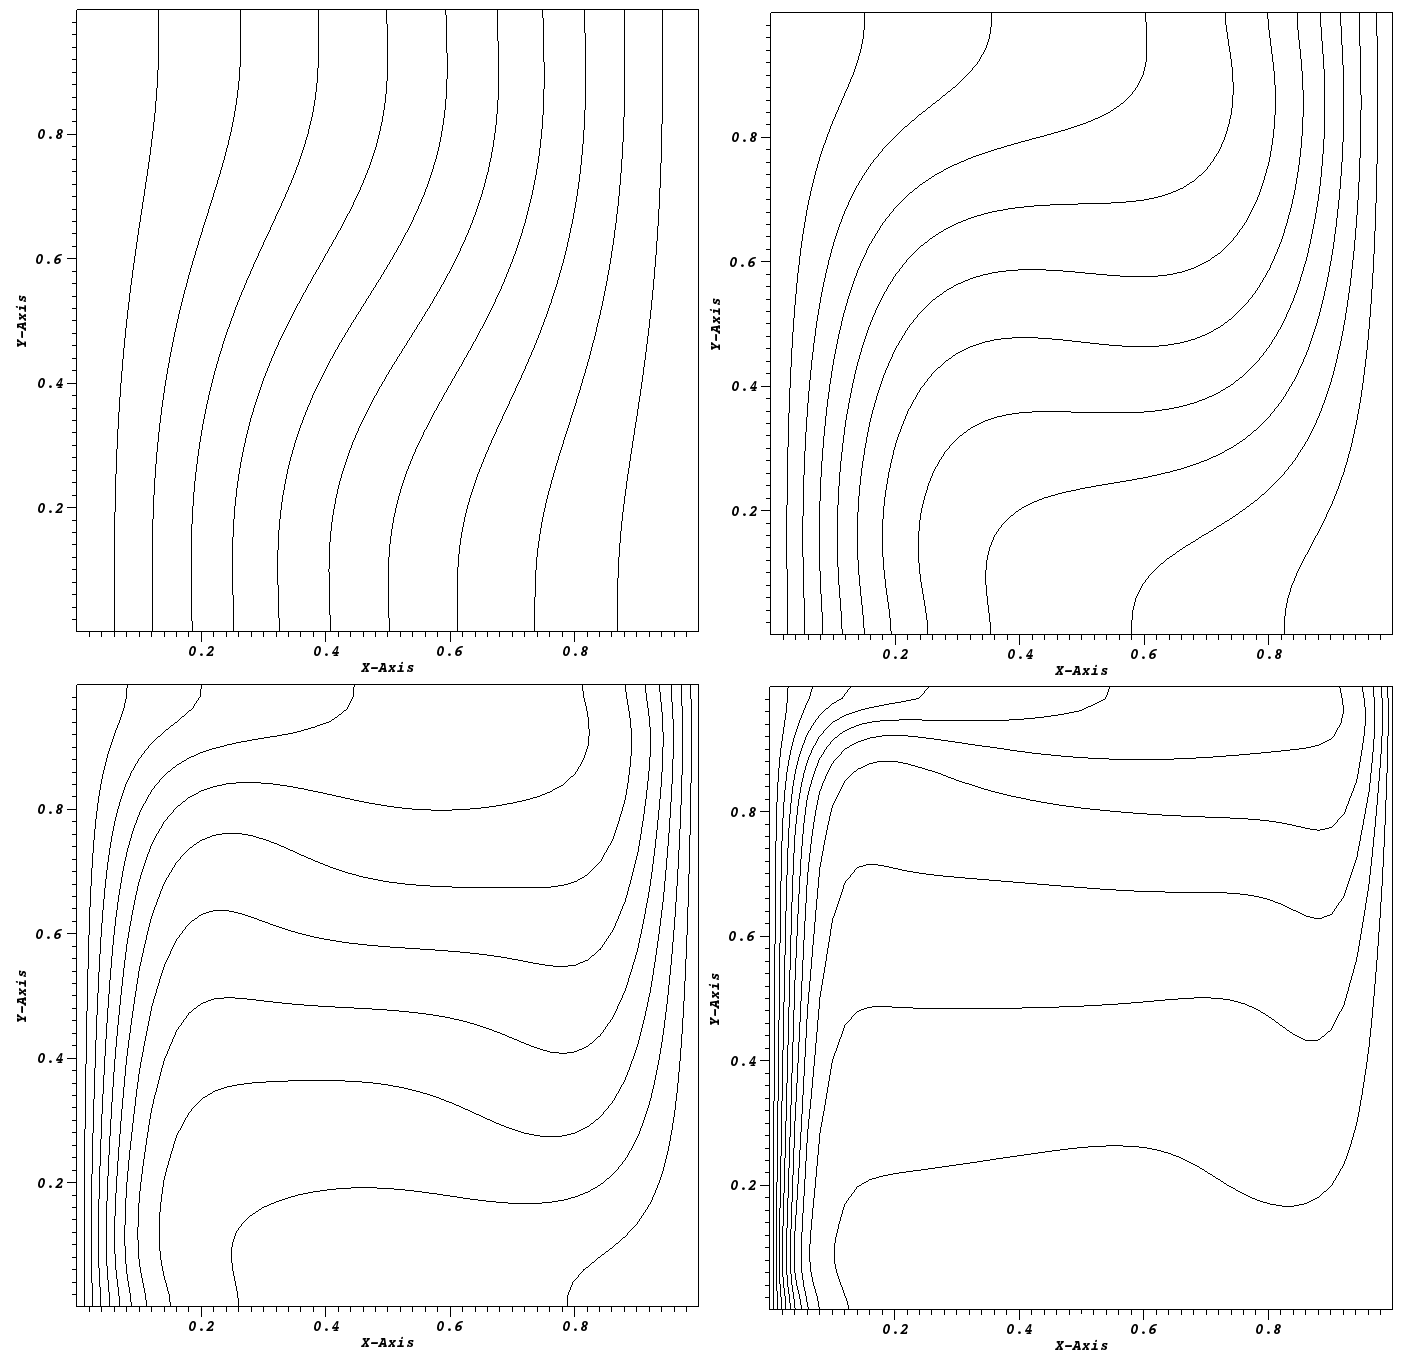
\includegraphics[width=6in]{chapters/nonlinear_problem/convection_isotherms.png}
  \end{center}
  \caption{\textbf{Isotherms from solution to the thermal convection
        cavity problem.} \textit{Top left: Ra = \sn{1}{3}; Top right:
        Ra = \sn{1}{4}; Bottom left: Ra = \sn{1}{5}; Bottom left: Ra =
        \sn{1}{6}. Isotherms on unit temperature scale from 0 to 1
        with divisions of 0.1 for each calculation.}}
  \label{fig:convection_isotherms}
\end{figure}

\clearpage

\subsection{Lid Driven Cavity Problem}
\label{subsec:lid_driven_cavity}
As an extension of the convection problem, the second benchmark
problem given by Ghia \citep{ghia_high-re_1982} adds a driver for the
flow to introduce higher Reynolds numbers into the system, providing
more inertial force to overcome the viscous forces in the fluid. The
setup for this problem is equally simple, containing only the
Dirichlet conditions as given in Figure~\ref{fig:lid_driven_cavity}
and is only applied to the mass and momentum equations on the unit
square.

\begin{figure}[t!]
  \begin{center}
    \scalebox{1.5}{
      \input{chapters/nonlinear_problem/lid_driven_cavity.pdftex_t} }
  \end{center}
  \caption{\textbf{Problem setup for the lid driven cavity benchmark.}
    \textit{Dirichlet conditions of zero are set for the velocity on
      the left and right and bottom while the Dirichlet condition set
      on the top provides a driving force on the fluid.}}
  \label{fig:lid_driven_cavity}
\end{figure}

The top boundary condition will provide a driver for the flow and its
variation will in turn vary the Reynolds number of the fluid. An
increased velocity will generate more inertial forces in the fluid,
which will overcome the viscous forces and again increase the
influence of the nonlinear terms in Eq~(\ref{eq:ns_momentum}). Shadid
used Reynolds numbers up to \sn{1}{4} for this benchmark problem.

Isocurves of the velocity magnitudes are given in
Figure~\ref{fig:driven_velocity_isocurves} for solutions to the lid
driven cavity problem at Reynolds numbers of 100, 300, 500 and
700. Increasing the velocity on the top boundary of the problem drives
up the Reynolds number of the system making it more difficult to
solve. More rotation of the fluid is induced by inertial forces and
we begin to see some additional vortices form besides the primary
vortex in the center of the box.

\begin{figure}[t!]
  \begin{center}
    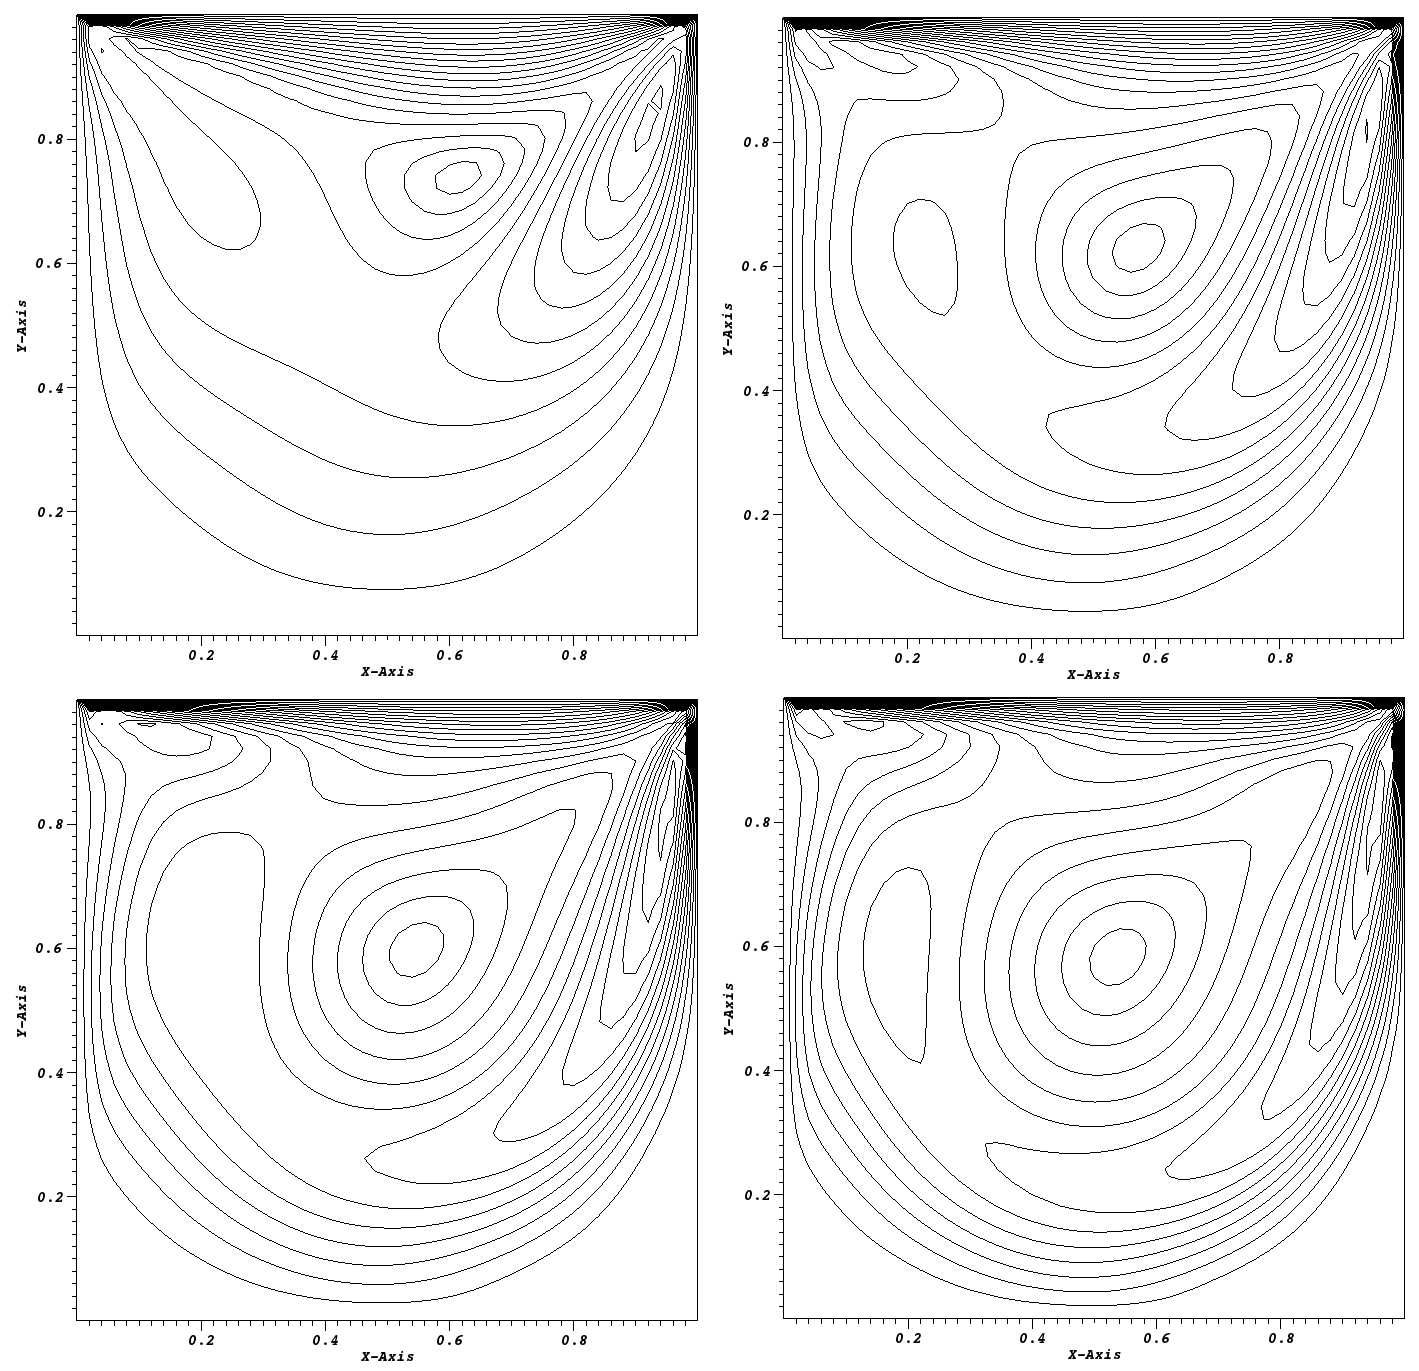
\includegraphics[width=6in]{chapters/nonlinear_problem/driven_velocity_isocurves.png}
  \end{center}
  \caption{\textbf{Velocity magnitude isocurves from solution to the
      thermal convection cavity problem.} \textit{Top left: Re = 100;
      Top right: Re= 300; Bottom left: Re = 500; Bottom left: Re =
      700. Isocurves on unit velocity scale from 0 to 1 with divisions
      of 0.05 for each calculation.}}
  \label{fig:driven_velocity_isocurves}
\end{figure}

\clearpage

%%---------------------------------------------------------------------------%%
\section{FANM Verification\ }
\label{sec:fanm_verification}

For each of the benchmark problems, we will present the results of
computations using FANM and directly compare them to results using a
Newton-Krylov method in order to verify the correctness of FANM and
its applicability to fluid problems. For each case, we will compare
the global minimum, maximum, and average values for fluid velocity,
pressure, and temperature where applicable. If the values for these
quantities computed using FANM match those computed using a production
Newton-Krylov method, the implementation will be deemed correct for
the purposes of this work. In addition, we will report the tolerance
to which the nonlinear residual was converged as an additional means
of comparison for correctness.

Given the difficulty of these benchmark problems, the linear solve at
each Newton step was preconditioned with an algebraic multigrid
method, a common technique for preconditioning these equations
\citep{ghia_high-re_1982,evans_enhanced_2007}. Without multigrid
preconditioning, the residual in MCSA was observed to
stagnate. Typically this happens because the Richardson iteration will
damp the higher order error modes on the scale of the computational
grid used to solve the problem but will miss lower order error
modes. In terms of Monte Carlo, this stagnation manifests itself in
histories that simply do no terminate and therefore no solution is
acquired.

For FANM, this preconditioning was required to reduce the spectral
radius of the Jacobian operators generated at each Newton step and for
the Newton-Krylov solutions this preconditioning was required to
obtain good convergence properties although it was not necessary for
convergence. For every benchmark calculation, both FANM and
Newton-Krylov were preconditioned with the same multigrid parameters
such that the conditioning of the system would not be a factor in the
verification of the method or the performance comparison in the
following section. As with the radiation transport calculations in the
previous chapter, algrebraic preconditioning with the multigrid method
results in dense linear systems. To mitigate this, the reduced domain
approximation was again applied to the Monte Carlo solution within the
MCSA solve occuring at each nonlinear iteration. The values used for
the approximation will be given for each benchmark problem.

Results in this and the following section were produced by the Drekar
multiphysics code base being developed at Sandia National Laboratories
for fluid flow and other multiple physics simulations
\citep{pawlowski_drekar_2012}. Drekar is a massively parallel physics
framework that utilizes Newton-Krylov methods to generate a fully
consistent solution scheme for the Navier-Stokes equations among other
systems with Jacobian generation through automatic differentiation. To
achieve these results, a Monte Carlo solver generated for this work
was injected into the nonlinear toolchain within Drekar to form an
implementation of the FANM method. For the Newton-Krylov solutions,
the same production implementation of GMRES from the Trilinos
scientific computing library Aztec \citep{heroux_overview_2005} used
for the verification of MCSA for the $SP_N$ solutions in the previous
chapter was also used here as a means of comparison and FANM
benchmarking.

\subsection{Thermal Convection Cavity Results}
\label{subsec:thermal_convection_verification}

A Drekar model of thermal convection cavity problem was solved using
both the Newton-Krylov solver and a FANM solver for Rayleigh numbers
of \sn{1}{3}, \sn{1}{4}, \sn{1}{5} and \sn{1}{6} on a $50 \times 50$
square grid. Table~\ref{tab:thermal_convection_parameters} gives the
physical parameters of the problem and
Table~\ref{tab:convection_mcsa_parameters} gives the MCSA solver
parameters used within the FANM method. Variation in the Rayleigh
number of the system was achieved by keeping the parameters given in
Table~\ref{tab:thermal_convection_parameters} constant and varying
temperature of the hot side of the cavity. In addition to multigrid
preconditioning for the linear solution at each Newton step,
backtracking as outlined in Shadid's work \citep{shadid_inexact_1997}
was used as a means of globalization to assist the Newton correction
computation while the forcing term was computed at each Newton step
using method 2 from Shadid's work. In this forcing term method,
nonlinear residuals from the two previous Newton steps are used to
inform the choice of the forcing term for the next step.

\begin{table}[h!]
  \begin{center}
    \begin{tabular}{lcc}\hline\hline
      \multicolumn{1}{l}{Parameter}& 
      \multicolumn{1}{c}{Value}&
      \multicolumn{1}{c}{Units}\\\hline
      $x_{min}$ & 0.0 & $m$ \\
      $x_{max}$ & 1.0 & $m$ \\
      $y_{min}$ & 0.0 & $m$ \\
      $y_{max}$ & 1.0 & $m$ \\
      $N_x$ & 50 & - \\
      $N_y$ & 50 & - \\
      $DOFs$ & 10404 & - \\
      Initial Temperature & 0.0 & $K$ \\
      Density & 1.0 & $kg / m^3$ \\
      Specific Heat & 1.0 & J / $(kg \times K)$ \\
      Dynamic Viscosity & 0.71 & $N \times s / m^2$ \\
      Thermal Conductivity & 1.0 & $W / (m \times K)$ \\
      Thermal Expansion Coefficient & 1000 & $1 / K$ \\
      Thermal Diffusivity & 1.0 & $m^2 / s$ \\
      Kinematic Viscosity & 0.71 & $m^2 / s$ \\
      Gravitational Acceleration & 10 & $m / s^2$ \\
      Cavity Characteristic Length & 1.0 & $m$ \\
      Prandtl Number & 0.71 & - \\
      %%
      \hline\hline
    \end{tabular}
  \end{center}
  \caption{\textbf{Thermal convection cavity FANM verification model
      problem parameters.}  \textit{The Navier-Stokes equations in 2
      dimensions are used for the model problem. The Rayleigh number
      is varied by modifying the hot boundary temperature to induce
      larger temperature gradients and bouyancy-driven flow.}}
  \label{tab:thermal_convection_parameters}
\end{table}

\begin{table}[h!]
  \begin{center}
    \begin{tabular}{lc}\hline\hline
      \multicolumn{1}{l}{Parameter}& 
      \multicolumn{1}{c}{Value}\\\hline
      Histories & 500,000 per iteration \\
      Weight Cutoff & \sn{1}{-2} \\
      Fixed Point Iteration & Richardson \\
      Estimator & Adjoint Collision \\
      Reduced Domain Fill Level & 200 \\
      %%
      \hline\hline
    \end{tabular}
  \end{center}
  \caption{\textbf{Thermal convection cavity FANM verification MCSA
      solver parameters.} \textit{No relaxation parameters or variance
      reduction techniques were used with MCSA other than the reduced
      domain approximation.}}
  \label{tab:convection_mcsa_parameters}
\end{table}

For the verification calculations, at each Rayleigh number variation
the global minimum, maximum, and average values were recorded for
fluid velocity in the x and y directions, fluid pressure, and fluid
temperature. Tables~\ref{tab:convection_ra1e3_results},
\ref{tab:convection_ra1e4_results},
\ref{tab:convection_ra1e5_results}, and
\ref{tab:convection_ra1e6_results} give the results of these
computations. It should be noted that the negative pressures computed
are due to a relative pressure being reported. For each of the data
points presented, both Newton-Krylov solutions and FANM solutions
computed identical numerical results for all of these global
values. No variation in solution was noted for each of the
computations larger than the tolerance of the converged nonlinear
residual norms given in
Table~\ref{tab:convection_residual_norm_comparison}. Variations in the
convergence behavior and differences in performance for these
solutions will be analyzed in the following section.

\begin{table}[h!]
  \begin{center}
    \begin{tabular}{lll}\hline\hline
      \multicolumn{1}{l}{Parameter}& 
      \multicolumn{1}{l}{Newton-Krylov Result}&
      \multicolumn{1}{l}{FANM Result}\\
      \hline
      Average $U_x$ & -1.288835730E-05 & -1.288835730E-05 \\
      Minimum $U_x$ & -3.677243960E+00 & -3.677243960E+00 \\
      Maximum $U_x$ & 3.688908550E+00 & 3.688908550E+00 \\
      \hline
      Average $U_y$ & 3.403670530E-02 & 3.403670530E-02 \\
      Minimum $U_y$ & -3.721178580E+00 & -3.721178580E+00 \\
      Maximum $U_y$ & 3.791483420E+00 & 3.791483420E+00 \\
      \hline
      Average $P$ & 2.345554770E+02 & 2.345554770E+02 \\
      Minimum $P$ & -5.509779180E+00 & -5.509779180E+00 \\
      Maximum $P$ & 4.994885560E+02 & 4.994885560E+02 \\
      \hline
      Average $T$ & 3.595148700E-02 & 3.595148700E-02 \\
      Minimum $T$ & 2.092448340E-04 & 2.092448340E-04 \\
      Maximum $T$ & 7.178874510E-02 & 7.178874510E-02 \\
      %%
      \hline\hline
    \end{tabular}
  \end{center}
  \caption{\textbf{Thermal convection cavity FANM verification for a
      Rayleigh number of \sn{1}{3}.} \textit{The values reported are
      global minima, maxima, and averages for each variable in the
      problem. The velocity is given in components in the $x$ and $y$
      directions.}}
  \label{tab:convection_ra1e3_results}
\end{table}

\begin{table}[h!]
  \begin{center}
    \begin{tabular}{lll}\hline\hline
      \multicolumn{1}{l}{Parameter}& 
      \multicolumn{1}{l}{Newton-Krylov Result}&
      \multicolumn{1}{l}{FANM Result}\\
      \hline
      Average $U_x$ & -7.489201240E-04 & -7.489201240E-04 \\
      Minimum $U_x$ & -1.607318000E+01 & -1.607318000E+01 \\
      Maximum $U_x$ & 1.669098270E+01 & 1.669098270E+01 \\
      \hline
      Average $U_y$ & 3.377624420E-01 & 3.377624420E-01 \\
      Minimum $U_y$ & -1.932174800E+01 & -1.932174800E+01 \\
      Maximum $U_y$ & 2.047326820E+01 & 2.047326820E+01 \\
      \hline
      Average $P$ & 1.861894950E+03 & 1.861894950E+03 \\
      Minimum $P$ & -3.353416240E+01 & -3.353416240E+01 \\
      Maximum $P$ & 4.440642810E+03 & 4.440642810E+03 \\
      \hline
      Average $T$ & 3.510568440E-01 & 3.510568440E-01 \\
      Minimum $T$ & 2.092448340E-04 & 2.092448340E-04 \\
      Maximum $T$ & 7.178874510E-02 & 7.178874510E-02 \\
      %%
      \hline\hline
    \end{tabular}
  \end{center}
  \caption{\textbf{Thermal convection cavity FANM verification for a
      Rayleigh number of \sn{1}{4}.} \textit{The values reported are
      global minima, maxima, and averages for each variable in the
      problem. The velocity is given in components in the $x$ and $y$
      directions.}}
  \label{tab:convection_ra1e4_results}
\end{table}

\begin{table}[h!]
  \begin{center}
    \begin{tabular}{lll}\hline\hline
      \multicolumn{1}{l}{Parameter}& 
      \multicolumn{1}{l}{Newton-Krylov Result}&
      \multicolumn{1}{l}{FANM Result}\\
      \hline
      Average $U_x$ & -2.043639370E-02 & -2.043639370E-02 \\
      Minimum $U_x$ & -3.814922470E+01 & -3.814922470E+01 \\
      Maximum $U_x$ & -3.814922470E+01 & -3.814922470E+01 \\
      \hline
      Average $U_y$ & 2.774864300E+00 & 2.774864300E+00 \\
      Minimum $U_y$ & -6.038682990E+01 & -6.038682990E+01 \\
      Maximum $U_y$ & 7.873873560E+01 & 7.873873560E+01 \\
      \hline
      Average $P$ & 1.324208380E+04 & 1.324208380E+04 \\
      Minimum $P$ & -1.390235490E+02 & -1.390235490E+02 \\
      Maximum $P$ & 3.559215530E+04 & 3.559215530E+04 \\
      \hline
      Average $T$ & 3.027827770E+00 & 3.027827770E+00 \\
      Minimum $T$ & 1.626405740E-02 & 1.626405740E-02 \\
      Maximum $T$ & 7.162571130E+00 & 7.162571130E+00 \\
      %%
      \hline\hline
    \end{tabular}
  \end{center}
  \caption{\textbf{Thermal convection cavity FANM verification for a
      Rayleigh number of \sn{1}{5}.} \textit{The values reported are
      global minima, maxima, and averages for each variable in the
      problem. The velocity is given in components in the $x$ and $y$
      directions.}}
  \label{tab:convection_ra1e5_results}
\end{table}

\begin{table}[h!]
  \begin{center}
    \begin{tabular}{lll}\hline\hline
      \multicolumn{1}{l}{Parameter}& 
      \multicolumn{1}{l}{Newton-Krylov Result}&
      \multicolumn{1}{l}{FANM Result}\\
      \hline
      Average $U_x$ & -1.802569840E-01 & -1.802569840E-01 \\
      Minimum $U_x$ & -6.292084130E+01 & -6.292084130E+01 \\
      Maximum $U_x$ & 2.951113240E+02 & 2.951113240E+02 \\
      \hline
      Average $U_y$ & 1.336398550E+01 & 1.336398550E+01 \\
      Minimum $U_y$ & -1.345663290E+02 & -1.345663290E+02 \\
      Maximum $U_y$ & 3.227873890E+02 & 3.227873890E+02 \\
      \hline
      Average $P$ & 6.354313840E+04 & 6.354313840E+04 \\
      Minimum $P$ & -1.356309630E+02 & -1.356309630E+02 \\
      Maximum $P$ & 2.316308730E+05 & 2.316308730E+05 \\
      \hline
      Average $T$ & 1.780727610E+01 & 1.780727610E+01 \\
      Minimum $T$ & 8.265788890E-02 & 8.265788890E-02 \\
      Maximum $T$ & 7.098873170E+01 & 7.098873170E+01 \\
      %%
      \hline\hline
    \end{tabular}
  \end{center}
  \caption{\textbf{Thermal convection cavity FANM verification for a
      Rayleigh number of \sn{1}{6}.} \textit{The values reported are
      global minima, maxima, and averages for each variable in the
      problem. The velocity is given in components in the $x$ and $y$
      directions.}}
  \label{tab:convection_ra1e6_results}
\end{table}

\begin{table}[h!]
  \begin{center}
    \begin{tabular}{lcc}\hline\hline
      \multicolumn{1}{l}{Rayleigh Number}& 
      \multicolumn{1}{c}{Newton Krylov $||\ve{F(\ve{u})}||$}&
      \multicolumn{1}{c}{FANM $||\ve{F(\ve{u})}||$}\\
      \hline
      \sn{1}{3} & \sn{4.542}{-14} & \sn{1.208}{-14} \\
      \sn{1}{4} & \sn{1.045}{-12} & \sn{7.012}{-13} \\
      \sn{1}{5} & \sn{1.784}{-12} & \sn{1.059}{-12} \\
      \sn{1}{6} & \sn{3.404}{-12} & \sn{3.479}{-12} \\
      %%
      \hline\hline
    \end{tabular}
  \end{center}
  \caption{\textbf{Thermal convection cavity nonlinear residual norm
      achieved convergence.} \textit{The results presented here were
      obtained from the benchmark verification calculations.}}
  \label{tab:convection_residual_norm_comparison}
\end{table}

\clearpage

\subsection{Lid Driven Cavity Results}
\label{subsec:lid_driven_verification}

A Drekar model of thermal convection cavity problem was solved using
both the Newton-Krylov solver and a FANM solver for Reynolds numbers
of 100, 300, 500, and 700 on a $50 \times 50$ square
grid. Table~\ref{tab:thermal_convection_parameters} gives the physical
parameters of the problem and
Table~\ref{tab:convection_mcsa_parameters} gives the MCSA solver
parameters used within the FANM method. Variation in the Reynolds
number of the system was achieved by keeping the parameters given in
Table~\ref{tab:thermal_convection_parameters} fixed and varying the
fluid velocity in the $x$ direction on the top boundary. In addition
to multigrid preconditioning for the linear solution at each Newton
step, a polynomial line search method was used as a means of
globalization assisting the Newton correction computation as outlined
by Pawlowski in \citep{pawlowski_globalization_2006} while the forcing
term was again computed using method 2 from Shadid's work
\citep{shadid_inexact_1997}.

\begin{table}[h!]
  \begin{center}
    \begin{tabular}{lcc}\hline\hline
      \multicolumn{1}{l}{Parameter}& 
      \multicolumn{1}{c}{Value}&
      \multicolumn{1}{c}{Units}\\\hline
      $x_{min}$ & 0.0 & $m$ \\
      $x_{max}$ & 1.0 & $m$ \\
      $y_{min}$ & 0.0 & $m$ \\
      $y_{max}$ & 1.0 & $m$ \\
      $N_x$ & 50 & - \\
      $N_y$ & 50 & - \\
      $DOFs$ & 7803 & - \\
      Density & 1.0 & $kg / m^3$ \\
      Dynamic Viscosity & 0.71 & $N \times s / m^2$ \\
      Kinematic Viscosity & 0.71 & $m^2 / s$ \\
      Gravitational Acceleration & 10 & $m / s^2$ \\
      Cavity Characteristic Length & 1.0 & $m$ \\
      %%
      \hline\hline
    \end{tabular}
  \end{center}
  \caption{\textbf{Lid driven cavity FANM verification model
      problem parameters.}  \textit{The Navier-Stokes equations in 2
      dimensions are used for the model problem. The Reynolds number
      is varied by modifying the velocity magnitude on the upper
      boundary to induce flow driven by inertial forces.}}
  \label{tab:lid_driven_parameters}
\end{table}

\begin{table}[h!]
  \begin{center}
    \begin{tabular}{lc}\hline\hline
      \multicolumn{1}{l}{Parameter}& 
      \multicolumn{1}{c}{Value}\\\hline
      Weight Cutoff & \sn{1}{-2} \\
      Fixed Point Iteration & Richardson \\
      Estimator & Adjoint Collision \\
      Histories, Re=100 & 500,000 per iteration \\
      Histories, Re=300 & 500,000 per iteration \\
      Histories, Re=500 & 500,000 per iteration \\
      Histories, Re=700 & 1,000,000 per iteration \\
      Reduced Domain Fill Level, Re=100 & 200 \\
      Reduced Domain Fill Level, Re=300 & 200 \\
      Reduced Domain Fill Level, Re=500 & 200 \\
      Reduced Domain Fill Level, Re=700 & 300 \\
      %%
      \hline\hline
    \end{tabular}
  \end{center}
  \caption{\textbf{Lid driven cavity FANM verification MCSA solver
      parameters.} \textit{No relaxation parameters or variance
      reduction techniques were used with MCSA other than the reduced
      domain approximation. Different values of fill level for the
      reduced domain approximation and histories per iteration were
      used at different Reynolds numbers due to convergence
      requirements.}}
  \label{tab:driven_mcsa_parameters}
\end{table}

In the literature on this benchmark, solutions at Reynolds numbers of
up to \sn{1}{4} were achieved using a variety of nonlinear solution
techniques. With the FANM method, at Reynolds numbers above 700
convergence of the linear iterations could not be achieved regardless
of how agressive the multigrid preconditioner was set. In these cases,
the Jacobian operators are ill-conditioned enough that even GMRES
converges slowly relative to the thermal convection cavity
benchmark. Therefore, the spectral radius limitation on MCSA is
extremely prohibitive in this case and others where transport driven
by inertial forces is dominant. Because of this, only solutions to
the lid driven cavity benchmark at Reynolds numbers of up to 700 are
presented.

For the verification calculations, at each Reynolds number variation
the global minimum, maximum, and average values were recorded for the
fluid velocity in the x and y directions and the fluid
pressure. Tables~\ref{tab:driven_re100_results},
\ref{tab:driven_re300_results}, \ref{tab:driven_re500_results}, and
\ref{tab:driven_re700_results} give the results of these
computations. As with the thermal convection problem, the negative
pressures computed are due to a relative pressure being reported. For
each of the data points given, both Newton-Krylov solutions and FANM
solutions computed identical numerical results for all of these global
values. The norm of the converged nonlinear residual for the
calculations is given in
Table~\ref{tab:driven_residual_norm_comparison}. All computed global
values were within these tolerances.

\begin{table}[h!]
  \begin{center}
    \begin{tabular}{lll}\hline\hline
      \multicolumn{1}{l}{Parameter}& 
      \multicolumn{1}{l}{Newton-Krylov Result}&
      \multicolumn{1}{l}{FANM Result}\\
      \hline
      Average $U_x$ & 1.165632320E-01 & 1.165632320E-01 \\
      Minimum $U_x$ & -2.423642920E+01 & -2.423642920E+01 \\
      Maximum $U_x$ & 9.742670880E+01 & 9.742670880E+01 \\
      \hline
      Average $U_y$ & 2.038480420E-02 & 2.038480420E-02 \\
      Minimum $U_y$ & -5.266315430E+01 & -5.266315430E+01 \\
      Maximum $U_y$ & 2.720044160E+01 & 2.720044160E+01 \\
      \hline
      Average $P$ & -1.656193900E+02 & -1.656193900E+02 \\
      Minimum $P$ & -9.635479370E+03 & -9.635479370E+03 \\
      Maximum $P$ & 1.854517020E+04 & 1.854517020E+04 \\
      %%
      \hline\hline
    \end{tabular}
  \end{center}
  \caption{\textbf{Lid driven cavity FANM verification for a Reynolds
      number of 100.} \textit{The values reported are global minima,
      maxima, and averages for each variable in the problem. The
      velocity is given in components in the $x$ and $y$ directions.}}
  \label{tab:driven_re100_results}
\end{table}

\begin{table}[h!]
  \begin{center}
    \begin{tabular}{lll}\hline\hline
      \multicolumn{1}{l}{Parameter}& 
      \multicolumn{1}{l}{Newton-Krylov Result}&
      \multicolumn{1}{l}{FANM Result}\\
      \hline
      Average $U_x$ & 3.382078040E-01 & 3.382078040E-01 \\
      Minimum $U_x$ & -9.467140360E+01 & -9.467140360E+01 \\
      Maximum $U_x$ & 2.895885380E+02 & 2.895885380E+02 \\
      \hline
      Average $U_y$ & 8.780242440E-02 & 8.780242440E-02 \\
      Minimum $U_y$ & -1.830156060E+02 & -1.830156060E+02 \\
      Maximum $U_y$ & 8.827373340E+01 & 8.827373340E+01 \\
      \hline
      Average $P$ & -2.830380160E+03 & -2.830380160E+03 \\
      Minimum $P$ & -2.352177540E+04 & -2.352177540E+04 \\
      Maximum $P$ & 9.254997120E+04 & 9.254997120E+04 \\
      %%
      \hline\hline
    \end{tabular}
  \end{center}
  \caption{\textbf{Lid driven cavity FANM verification for a Reynolds
      number of 300.} \textit{The values reported are global minima,
      maxima, and averages for each variable in the problem. The
      velocity is given in components in the $x$ and $y$ directions.}}
  \label{tab:driven_re300_results}
\end{table}

\begin{table}[h!]
  \begin{center}
    \begin{tabular}{lll}\hline\hline
      \multicolumn{1}{l}{Parameter}& 
      \multicolumn{1}{l}{Newton-Krylov Result}&
      \multicolumn{1}{l}{FANM Result}\\
      \hline
      Average $U_x$ & 5.098921320E-01 & 5.098921320E-01 \\
      Minimum $U_x$ & -1.731861690E+02 & -1.731861690E+02 \\
      Maximum $U_x$ & 4.789146040E+02 & 4.789146040E+02 \\
      \hline
      Average $U_y$ & 1.365493140E-01 & 1.365493140E-01 \\
      Minimum $U_y$ & -3.170930360E+02 & -3.170930360E+02 \\
      Maximum $U_y$ & 1.655401440E+02 & 1.655401440E+02 \\
      \hline
      Average $P$ & -9.378317550E+03 & -9.378317550E+03 \\
      Minimum $P$ & -4.155215280E+04 & -4.155215280E+04 \\
      Maximum $P$ & 2.058742010E+05 & 2.058742010E+05 \\
      %%
      \hline\hline
    \end{tabular}
  \end{center}
  \caption{\textbf{Lid driven cavity FANM verification for a
      Reynolds number of 500.} \textit{The values reported are
      global minima, maxima, and averages for each variable in the
      problem. The velocity is given in components in the $x$ and $y$
      directions.}}
  \label{tab:driven_re500_results}
\end{table}

\begin{table}[h!]
  \begin{center}
    \begin{tabular}{lll}\hline\hline
      \multicolumn{1}{l}{Parameter}& 
      \multicolumn{1}{l}{Newton-Krylov Result}&
      \multicolumn{1}{l}{FANM Result}\\
      \hline
      Average $U_x$ & 6.479541170E-01 & 6.479541170E-01 \\
      Minimum $U_x$ & -2.550685400E+02 & -2.550685400E+02 \\
      Maximum $U_x$ & 6.663054900E+02 & 6.663054900E+02 \\
      \hline
      Average $U_y$ & 1.833690840E-01 & 1.833690840E-01 \\
      Minimum $U_y$ & -4.491052980E+02 & -4.491052980E+02 \\
      Maximum $U_y$ & 2.474376340E+02 & 2.474376340E+02 \\
      \hline
      Average $P$ & 1.833690840E-01 & 1.833690840E-01 \\
      Minimum $P$ & -6.241704500E+04 & -6.241704500E+04 \\
      Maximum $P$ & 3.518174810E+05 & 3.518174810E+05 \\
      %%
      \hline\hline
    \end{tabular}
  \end{center}
  \caption{\textbf{Lid driven cavity FANM verification for a Reynolds
      number of 700.} \textit{The values reported are global minima,
      maxima, and averages for each variable in the problem. The
      velocity is given in components in the $x$ and $y$ directions.}}
  \label{tab:driven_re700_results}
\end{table}

\begin{table}[h!]
  \begin{center}
    \begin{tabular}{lcc}\hline\hline
      \multicolumn{1}{l}{Reynolds Number}& 
      \multicolumn{1}{c}{Newton Krylov $||\ve{F(\ve{u})}||$}&
      \multicolumn{1}{c}{FANM $||\ve{F(\ve{u})}||$}\\
      \hline
      100 & \sn{5.453}{-14} & \sn{6.577}{-14} \\
      300 & \sn{2.537}{-13} & \sn{2.779}{-13} \\
      500 & \sn{6.367}{-13} & \sn{6.252}{-13} \\
      700 & \sn{9.159}{-13} & \sn{1.282}{-12} \\
      %%
      \hline\hline
    \end{tabular}
  \end{center}
  \caption{\textbf{Lid driven cavity nonlinear residual norm
      achieved convergence.} \textit{The results presented here were
      obtained from the benchmark verification calculations.}}
  \label{tab:driven_residual_norm_comparison}
\end{table}

\clearpage

%%---------------------------------------------------------------------------%%
\section{FANM Performance Comparison to Conventional Methods\ }
\label{sec:fanm_comparison}

Using the benchmarks from the verification, we now compare the
performance of the FANM method against a conventional Newton-Krylov
method. For each benchmark, we will analyze the iterative performance
of both the Newton solver and the linear solver used to compute the
correction vector at each step. In addition, timing results will be
discussed.

\subsection{Thermal Convection Cavity Results}
\label{subsec:thermal_convection_comparison}

At each Rayleigh number used for the thermal convection cavity
problem, Table~\ref{tab:convection_nonlinear_iter_comparison} gives
the number of Newton iterations required for convergence for each
method. Limiting the number of nonlinear iterations required for
solution is critical for efficiency as nonlinear function evaluations,
Jacobian generation, and preconditioner construction are typically
required at every Newton iteration. For all Rayleigh numbers except
\sn{1}{5} the number of Newton iterations required to converge is the
same while the \sn{1}{5} result required an extra FANM iteration. This
is due to the fact that the convergence of the linear residual has a
strong effect on the convergence of the nonlinear residual, much
stronger than the effect on the convergence of the eigenvalue in the
$SP_N$ computations where we observed that identical numbers of
eigenvalue iterations were required to converge each variation of the
probem.

As outlined in our discussion on inexact Newton methods, depending on
how converged the linear residual is at each step, it is possible to
throw off the nonlinear iteration and decrease iterative
performance. Although the same preconditioner was used with both the
Newton-Krylov and FANM calculations, the convergence properties of
MCSA and GMRES are different and we therefore expect them to produce
different results at each nonlinear iteration which will in turn
affect the forcing term calculation. If they are different enough, it
is possible that another Newton iteration may be required. Even
considering the extra Newton iteration, the solutions are converged to
effectively the same residual norm tolerance and produce the same
results as provided by the verification.

Figure~\ref{fig:ra1e5_convergence} gives the nonlinear residual
behavior for the \sn{1}{5} Rayleigh number case that required the
extra FANM iteration. We see that the extra iteration comes from
slightly slower quadratic convergence with FANM for this particular
case. The difference in convergence of the nonlinear problem comes
from the fact that the same multigrid preconditioner parameters are
used for this case as for the \sn{1}{3} and \sn{1}{4} Rayleigh number
cases for the linear solutions. Using the same preconditioner for the
harder \sn{1}{5} case means that the problem is still growing in
difficulty even though it is preconditioned. The more ill-conditioned
the linear model is, the closer the linear residual is converged to
the requested tolerance whereas a better conditioned problem may
produce a linear solution that overshoots the specified tolerance
provided by the forcing term. When oversolving is not an issue, this
results in faster convergence of the nonlinear problem.

For the \sn{1}{5} Rayleigh number case, this means that the GMRES
solver at each Newton step is converging the linear residual to a
smaller tolerance than the MCSA solver, even though they have
approximately the same forcing terms to begin with. As the Rayleigh
number increases, the problem becomes more difficult to solve and
therefore a more agressive preconditioner should maintain iterative
performance of the nonlinear method. This was observed to be true for
the \sn{1}{6} Rayleigh number case. For this calculation, the number
of multigrid cycle applications was bumped up to 3 from 1 and FANM
converged in the same number of nonlinear iterations as the
Newton-Krylov method.

\begin{table}[h!]
  \begin{center}
    \begin{tabular}{lcc}\hline\hline
      \multicolumn{1}{l}{Rayleigh Number}& 
      \multicolumn{1}{c}{Newton-Krylov Iterations}&
      \multicolumn{1}{c}{FANM Iterations}\\
      \hline
      \sn{1}{3} & 5 & 5 \\
      \sn{1}{4} & 7 & 7 \\
      \sn{1}{5} & 9 & 10 \\
      \sn{1}{6} & 11 & 11 \\
      %%
      \hline\hline
    \end{tabular}
  \end{center}
  \caption{\textbf{Thermal convection cavity nonlinear iteration
      results for the performance comparison.} \textit{The results
      presented here were obtained from the benchmark verification
      calculations.}}
  \label{tab:convection_nonlinear_iter_comparison}
\end{table}

\begin{figure}[htpb!]
  \begin{center}
    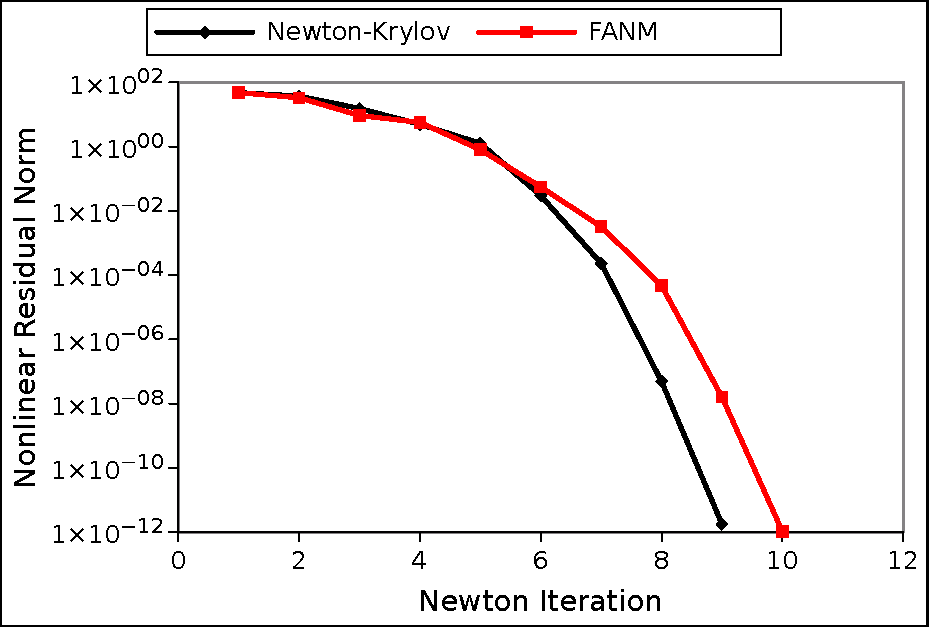
\includegraphics[width=6in]{chapters/nonlinear_problem/ra_1e5_convergence.pdf}
  \end{center}
  \caption{\textbf{Nonlinear residual norm as a function of Newton
      iteration for the \sn{1}{5} Rayleigh number case.} \textit{The
      FANM calculation required an additional nonlinear iteration to
      converge.}}
  \label{fig:ra1e5_convergence}
\end{figure}

In addition to nonlinear iterative performance, performance of the
inner linear solves is also interest. Here, we seek to maintain a
minimum number of total linear solver iterations over the course of
all nonlinear
iterations. Table~\ref{tab:convection_linear_iter_comparison} gives
the total number of GMRES iterations required to converge the problem
for the Newton-Krylov method and the total number of MCSA iterations
for the FANM method at each Rayleigh number used. For all cases, fewer
MCSA iterations were required than GMRES iterations to converge the
problem even with both solvers preconditioned with the same multigrid
package and the same parameters. For the \sn{1}{6} Rayleigh number
case this difference is most drastic with FANM requiring only 64\% of
the linear iterations required by the Newton-Krylov scheme. Even the
\sn{1}{5} Rayleigh number case that required more Newton iterations
required 5 fewer MCSA iterations to converge than GMRES iterations.

\begin{table}[h!]
  \begin{center}
    \begin{tabular}{lcc}\hline\hline
      \multicolumn{1}{l}{Rayleigh Number}& 
      \multicolumn{1}{c}{GMRES Iterations}&
      \multicolumn{1}{c}{MCSA Iterations}\\
      \hline
      \sn{1}{3} & 23 & 18 \\
      \sn{1}{4} & 23 & 17 \\
      \sn{1}{5} & 25 & 20 \\
      \sn{1}{6} & 39 & 25 \\
      %%
      \hline\hline
    \end{tabular}
  \end{center}
  \caption{\textbf{Thermal convection cavity total sum of linear
      iterations for all nonlinear iterations.} \textit{The results
      presented here were obtained from the benchmark verification
      calculations.}}
  \label{tab:convection_linear_iter_comparison}
\end{table}

Although the iterative performance of FANM is excellent for the
thermal convection cavity problem, the explicit preconditioning
strategy causes the same issues as was observed for the $SP_N$
equations in the previous
chapter. Table~\ref{tab:convection_speedup_comparison} gives the
speedup of the Newton-Krylov method over FANM. For all Rayleigh
numbers, we see a fairly constant speedup of O(400) when using
Newton-Krylov over FANM meaning that the implementation of the FANM
method used here is significantly slower. As the inexact Newton scheme
in Drekar was modified by simply swapping out the linear solver used
at each Newton step, this increased compute time is coming directly
from using MCSA as the solver and the overhead due to
preconditioning. When preconditioning overhead for the $SP_N$
equations was considered as shown by the data in
Figure~\ref{fig:spn_comparison_prec_time}, a similar speedup of
approximately two orders of magnitude was noted between the Krylov
methods and MCSA showing consistency between those results and the
fluid benchmark results. In addition, the fairly constant speedup
values as a function of the primary problem parameter show that FANM
has effectively the same time complexity as a Newton-Krylov method and
the implementation timings simply differ by a constant value.

\begin{table}[h!]
  \begin{center}
    \begin{tabular}{lcc}\hline\hline
      \multicolumn{1}{l}{Rayleigh Number}& 
      \multicolumn{1}{c}{Newton-Krylov Speedup}\\
      \hline
      \sn{1}{3} & 338 \\
      \sn{1}{4} & 336 \\
      \sn{1}{5} & 346 \\
      \sn{1}{6} & 465 \\
      %%
      \hline\hline
    \end{tabular}
  \end{center}
  \caption{\textbf{Thermal convection cavity Newton-Krylov speedup
      over FANM method.} \textit{Speedup values are rounded to the
      nearest integer. The results presented here were obtained from
      the benchmark verification calculations.}}
  \label{tab:convection_speedup_comparison}
\end{table}

\clearpage

\subsection{Lid Driven Cavity Results}
\label{subsec:lid_driven_comparison}

For the lid driven cavity benchmark, performance results were again
compared between the FANM and Newton-Krylov calculations. In this
case, the nonlinear iterative performance results as given by
Table~\ref{tab:driven_nonlinear_iter_comparison} show that the same
number of Newton iterations were required to converge the 100, 300,
and 500 Reynolds number cases while the FANM calculation with a
Reynolds number of 700 actually converged in 4 fewer iterations. The
nonlinear residual norm as a function of Newton iteration for this
case is given in Figure~\ref{fig:re700_convergence}.

This result can be explained by the fact that as given by
Table~\ref{tab:driven_mcsa_parameters}, although the preconditioner
parameters were the same for both calculations, the MCSA iteration was
pushed harder by doubling the number of histories used for the
computation at each nonlinear iteration. These extra histories
provided better convergence of the linear model at each iteration and
did not result in oversolving, thereby increasing the convergence rate
of the nonlinear model as well.

\begin{table}[h!]
  \begin{center}
    \begin{tabular}{lcc}\hline\hline
      \multicolumn{1}{l}{Reynolds Number}& 
      \multicolumn{1}{c}{Newton-Krylov Iterations}&
      \multicolumn{1}{c}{FANM Iterations}\\
      \hline
      100 & 6 & 6 \\
      300 & 9 & 9 \\
      500 & 11 & 11 \\
      700 & 14 & 10 \\
      %%
      \hline\hline
    \end{tabular}
  \end{center}
  \caption{\textbf{Lid driven cavity nonlinear iteration
      results for the performance comparison.} \textit{The results
      presented here were obtained from the benchmark verification
      calculations.}}
  \label{tab:driven_nonlinear_iter_comparison}
\end{table}

\begin{figure}[htpb!]
  \begin{center}
    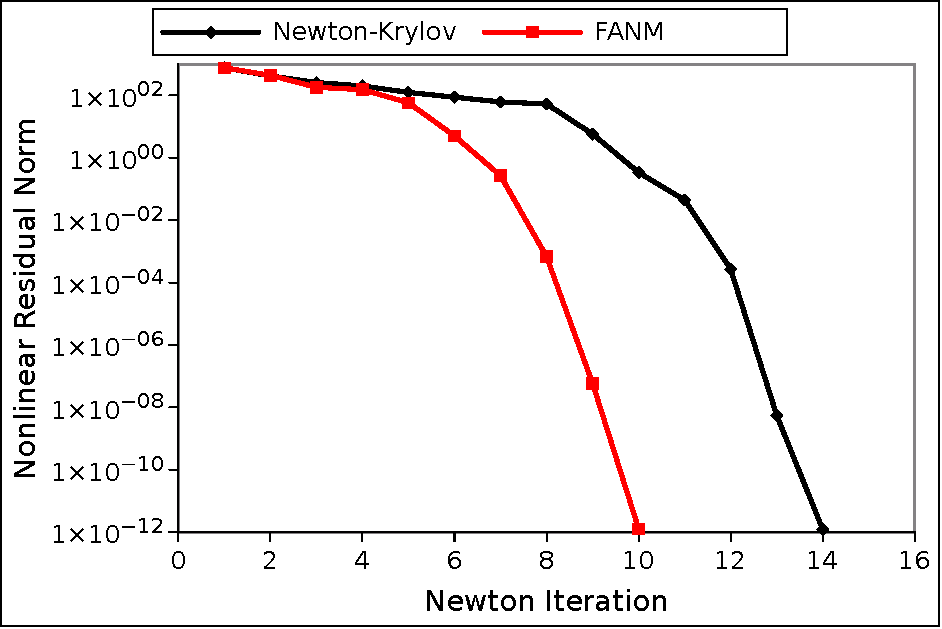
\includegraphics[width=6in]{chapters/nonlinear_problem/re700_convergence.pdf}
  \end{center}
  \caption{\textbf{Nonlinear residual norm as a function of Newton
      iteration for the 700 Reynolds number case.} \textit{The FANM
      calculation converged in 4 fewer iterations than the
      Newton-Krylov calculation.}}
  \label{fig:re700_convergence}
\end{figure}

The difficulty of this benchmark problem as compared to the thermal
convection cavity problem is readily apparent in the linear iteration
counts as given by Table~\ref{tab:driven_linear_iter_comparison}. As
the opposite of what was observed for that benchmark, lid driven
cavity results show that the linear models were significantly more
ill-conditioned, requiring many more MCSA and GMRES iterations. For
all cases except the 700 Reynolds number case, many more MCSA
iterations were required to converge with the observed GMRES iteration
count 64\% of that observed for MCSA when looking at the 100 Reynolds
number case. For the 700 Reynolds number case, fewer MCSA iterations
were observed due to the fact that 4 fewer nonlinear iterations were
performed. The average number of linear iterations per nonlinear
iteration was still much larger for the FANM calculations.

These iterative results again point out the fundamental flaw of
requiring a spectral radius of less than unity for the MCSA iteration
to converge at each Newton step. As the problem becomes more dominated
by inertial forces, the resulting linear models become increasingly
stiff and difficult to precondition. As a result, convergence requires
many more iterations than needed for the flow problem driven by
convection in the previous benchmark if convergence is achieved at
all.

\begin{table}[h!]
  \begin{center}
    \begin{tabular}{lcc}\hline\hline
      \multicolumn{1}{l}{Reynolds Number}& 
      \multicolumn{1}{c}{GMRES Iterations}&
      \multicolumn{1}{c}{MCSA Iterations}\\
      \hline
      100 & 27 & 42 \\
      300 & 35 & 52 \\
      500 & 41 & 56 \\
      700 & 21 & 14 \\
      %%
      \hline\hline
    \end{tabular}
  \end{center}
  \caption{\textbf{Lid driven cavity total sum of linear
      iterations for all nonlinear iterations.} \textit{The results
      presented here were obtained from the benchmark verification
      calculations.}}
  \label{tab:driven_linear_iter_comparison}
\end{table}

As a final comparison, the timing of both methods was again compared
with the speedup of using the Newton-Krylov solver over FANM reported
in Table~\ref{tab:driven_speedup_comparison}. The speedup values
reported here are of the same magnitude as those reported for the
thermal convection cavity problem and in agreement with those observed
for the $SP_N$ calculations. In all cases, the preconditioning
strategy must be signficantly improved to avoid these large overheads.

\begin{table}[h!]
  \begin{center}
    \begin{tabular}{lcc}\hline\hline
      \multicolumn{1}{l}{Reynolds Number}& 
      \multicolumn{1}{c}{Newton-Krylov Speedup}\\
      \hline
      100 & 299 \\
      300 & 322 \\
      500 & 288 \\
      700 & 488 \\
      %%
      \hline\hline
    \end{tabular}
  \end{center}
  \caption{\textbf{Lid driven cavity Newton-Krylov speedup
      over FANM method.} \textit{Speedup values are rounded to the
      nearest integer. The results presented here were obtained from
      the benchmark verification calculations.}}
  \label{tab:driven_speedup_comparison}
\end{table}

%%---------------------------------------------------------------------------%%
\section{Summary}
\label{sec:nonlinear_summary}

In this chapter we have developed and explored Monte Carlo synthetic
acceleration methods in the context of solutions to the nonlinear
Navier-Stokes equations. The following are the signficant observations
and findings.

\begin{itemize}
\item Forward-Automated Newton-MCSA (FANM), a new inexact Newton
  method based on Monte Carlo synthetic acceleration, has been
  developed
\item The FANM method has been incorporated into the Drekar production
  multiphysics code
\item The FANM method has been verified to produce the same solutions
  as a production Newton-Krylov method for two benchmark problems for
  the Navier-Stokes equations in different flow regimes
\item The FANM method has better iterative performance than the
  Newton-Krylov method for convection dominated problems, converging
  in fewer linear solver iterations with the same preconditioning for
  high and lower Rayleigh numbers
\item The Newton-Krylov method has better iterative performance than
  the FANM method for flow dominated by interial forces, converging in
  fewer linear solver iterations with the same preconditioning
\item The spectral radius convergence restriction on MCSA was observed
  to be a signficant hinderance by preventing solutions to forced flow
  problems at high Reynolds numbers
\item Explict algebraic preconditioning of MCSA creates FANM run times
  $O(100)$ slower than the Newton-Krylov solver
\item More Monte Carlo histories at every FANM iteration can reduce
  the number of linear and nonlinear iterations required to converge
  the problem
\end{itemize}

\blankpage
\chapter{Monte Carlo Solution Methods for the Navier-Stokes Equations}
\label{ch:mc_ns_solutions}

Put Navier Stokes work here.

\blankpage
\chapter{Research Proposal}
\label{ch:research_proposal}

After all of the background information and explanations of the new
work, this section is the most important of all. Here I will clearly
define the questions I aim to answer and the strategy that I will use
to attempt to answer them.

\section{Progress to Date}
\label{sec:progress}

\subsection{Generalization of MCSA for Linear Problems}
\label{subsec:mcsa_generalization}

\subsection{Direct vs. Adjoint Analysis}
\label{subsec:mcsa_direct_vs_adjoint}

\subsection{MCSA Application to Finite Element Problems}
\label{subsec:mcsa_finite_element}

\section{Key Questions}
\label{sec:key_questions}

\section{Solution Strategies}
\label{seq:solution_strategies}


%% etc, etc.

%% Do you have appendices?  If so, add them here, just like chapters.
% \begin{appendices}
% \include{backmatter/appendix1}
% \end{appendices}

%% Are you a big nerd with a colophon?  Add it here.
%% \begin{colophon}
%% \svnidlong{$LastChangedBy$}{$LastChangedRevision$}{$LastChangedDate$}{$HeadURL: http://freevariable.com/dissertation/trunk/frontmatter.tex $}
\vcinfo{}

This template uses Gyre Pagella by default.  (I used Arno Pro in my dissertation.)

Feel free to give me a shout-out in your colophon or acks if this template is useful for you.  Good luck!

%% \end{colophon}

%% McBride is a very nice style (some version is included in this
%% distribution)
\blankpage
\bibliographystyle{mcbride}
\bibliography{references}

%% Want an index?  Neither did I.
\printindex

\end{document}
